%% final_thesis.tex
%% PhD Dissertation — Héctor Carrión — UC Santa Cruz — June 2026
%% Based on the UCSC ucthesis class used in the advancement proposal,
%% extended to incorporate the cgDDI and DermDepth works.

\PassOptionsToPackage{table}{xcolor}
\documentclass[11pt]{ucthesis}
\def\dsp{\def\baselinestretch{2.0}\large\normalsize}
\dsp

% ---- Core packages (carried over from advancement thesis) ----------
\usepackage{amsmath}
\usepackage{amssymb}
\usepackage{graphicx}
\usepackage{caption}
\usepackage{subcaption}
\usepackage{booktabs}

% ---- Additional packages needed for cgDDI and DermDepth chapters ---
\usepackage{threeparttable}
\usepackage{multirow}
\usepackage{makecell}
\usepackage{colortbl}
\usepackage{xcolor}
\usepackage{siunitx}
\usepackage{xspace}
\usepackage[hidelinks]{hyperref}
\usepackage[capitalize,noabbrev]{cleveref}

% ---- Math operators / shortcuts (single declaration) --------------
\DeclareMathOperator*{\argmax}{argmax}
\newcommand{\ie}{\textit{i.e.}\xspace}
\newcommand{\eg}{\textit{e.g.}\xspace}
\newcommand{\etal}{\textit{et al.}\xspace}
\newcommand{\wrt}{w.r.t.\xspace}
\newcommand{\DDS}{DermDepth\textsubscript{S}}


\begin{document}

% ============================================================
% Front Matter
% ============================================================

\title{Deep Learning Algorithms for Medical Image Representation Learning and Understanding}
\author{Héctor Carrión}
\degree{Doctor of Philosophy}
\degreeyear{2026}
\degreemonth{June}
\chair{Professor Narges Norouzi}
\committeememberone{Professor Marcella Gomez}
\committeemembertwo{Professor Leilani H. Gilpin}
\numberofmembers{3}
\deanlineone{Peter Biehl}
\deanlinetwo{Vice Provost and Dean of Graduate Studies}
\deanlinethree{}
\field{Computer Science and Engineering}
\campus{Santa Cruz}

\begin{frontmatter}

\maketitle
%\copyrightpage

\begin{abstract}
Medical image analysis is constrained by a structural mismatch: clinical decision-making demands fine-grained understanding across diverse populations, body sites, and disease severities, yet expert annotations are scarce, demographic coverage is uneven, and rare presentations are nearly absent. This dissertation develops deep learning algorithms that compensate for that mismatch through four connected works in dermatology and wound care, domains where the limitations are most acute, and the downstream stakes for under-imaged populations are highest. We develop four methods spanning unsupervised, self-supervised, and supervised strategies, with both non-parametric and parametric generative paradigms. When there are no labels, we learn unsupervised from temporal structure (HealNet); when there is no temporal structure, we learn supervised from a frozen diffusion backbone (FEDD); when the data themselves are too few and too imbalanced, we generate them with sensitive-attribute control (cgDDI); and to close the loop into 3D space, we develop metric scale dermatology foundation models with non-parametric synthetic and real data (DermDepth).

\textbf{HealNet} introduces a self-supervised framework for acute wound heal-stage classification, learning biologically meaningful temporal embeddings without any human-provided labels and reaching 97.7\% pre-text and 90.6\% downstream stage-classification accuracy on a small longitudinal cohort. \textbf{FEDD} generalizes representation learning to the single-image clinical setting by re-tasking a frozen denoising-diffusion backbone as the encoder, achieving state-of-the-art segmentation (IoU lift 0.06--0.18) and a 14-point gain in malignancy classification accuracy on the biopsy-confirmed Diverse Dermatology Images (DDI) benchmark while using only 5--20\% of the available labels, and contributes the first explicit skin-tone-stratified fairness evaluation of the work. \textbf{cgDDI} repurposes that diffusion backbone as a controllable generator, combining latent-diffusion in-painting, non-parametric lesion mapping, and textual-inversion plus LoRA prior-preservation to grow a 656-image dataset by over $400\times$, balancing the full Fitzpatrick spectrum and lifting DDI malignancy classification to state-of-the-art 90.9\% accuracy with EOM fairness 86.6 (up from 69.6) and a $+13.9$\% cross-dataset gain on Fitzpatrick17k. \textbf{DermDepth} closes the loop from 2D to 3D, presenting the first single-view metric-scale 3D reconstruction model for dermatology together with \textbf{D-Synth}, the first synthetic dermoscopic dataset with pixel-perfect depth, normals, and camera intrinsics; a 2.1\,M-parameter scale-and-normal head on top of a frozen MoGe-2 backbone corrects metric scale error from over $16\times$ to under $1.1\times$ on real dermoscopic data, reduces skin-tone scale disparity from $10.90$ to $1.02$, and validates 3D lesion width, area, and volume estimation across SKINL2, WoundsDB, and DDI against the published clinical literature.

Across the work, a pattern recurs: small, clean datasets; frozen large backbones with trainable heads; and explicit, skin-tone-stratified fairness evaluation. We believe this framework generalizes beyond dermatology to any data-constrained medical imaging domain. All synthetic data, fine-tuned checkpoints, annotation work, code, and per-disease generative models are released openly to support reproducibility and continued fairness research.
\end{abstract}

\tableofcontents
\listoffigures
\listoftables

\end{frontmatter}

% ============================================================
% Chapter 1 — Introduction
% ============================================================
\chapter{Introduction}\label{section:intro}

Recent advancements in computational methods have ushered in a new era of scientific innovation, primarily driven by Machine Learning (ML), Deep Learning (DL), and, more broadly, Artificial Intelligence (AI). These technologies have become pivotal in reshaping various fields, including healthcare, where they hold the potential to improve the quality of patient care. The integration of AI into clinical practice has shown enhancements in disease diagnosis, treatment selection, and patient engagement \cite{Alowais2023RevolutionizingHT}.

In the biomedical domain, AI algorithms have demonstrated the ability to predict the onset and progression of diseases, develop personalized treatment plans, aid clinicians in the decision-making processes, and thus improve patient outcomes \cite{hema_2022, ahsan_2022, gopi_2020, Delpino2022MachineLF, Myszczynska2020ApplicationsOM}. While there exists a broad range of medical processes that can benefit from these advancements, key among them is multi-modal biomedical image representation learning, processing, and understanding.

Visual examination of a disease is often the very first step towards treatment. This is evidently true for external medical conditions such as skin lesions, wounds, and burns, but medical research has also developed several advanced imaging techniques to observe internal conditions. For instance, Magnetic Resonance Imaging (MRI), Computed Tomography (CT), X-Ray imaging, and ultrasonography scanners are actively used in clinical practice for internal conditions \cite{Hussain2022ModernDI, Li2020ImagingIC}. External conditions are primarily imaged using color cameras (RGB); however, the field has seen a diversification in data collection modalities, ranging from cell-phones to professional digital single-lens reflex cameras (DSLR) and recently toward custom-built camera monitoring systems \cite{Li2023ProgrammableDO}. Consequently, researchers and practitioners have collected dermatological data via differing modalities \cite{data_dryad}. This diversification reflects the growing need for adaptable, robust, and accurate multimodal imaging understanding systems in medical practice.

Discriminative AI and Computer Vision (CV), in combination with DL, has shown significant effectiveness in many visual tasks: image classification, object detection, inpainting, semantic segmentation, and representation learning, which is broadly defined as the practice of encoding meaningful image representations useful for downstream tasks \cite{Chai2021DeepLI, chen2020simple, chen2020big}. Ongoing CV and DL research, advancements in computing power, and, crucially, the availability of large labelled datasets have significantly contributed toward the growth, capabilities, and performance of artificial intelligence computer models for image understanding in recent years.

Generative AI has recently seen the emergence of Denoising Diffusion Probabilistic Models (DDPMs) \cite{Ho2020DenoisingDP}, a novel form of modeling that has improved various aspects of image processing and synthesis. DDPMs work by first iteratively adding noise to a target data distribution (following a Markov chain process), then learning to gradually remove this noise step-by-step back to the original data. Thus, the model transitions from a simple distribution (like Gaussian noise) into a complex data distribution (such as natural images) through a sequence of reverse diffusion steps. Each step involves a slight modification of the noisy data, guided by a neural network that learns to reverse this diffusion process. This approach has shown an ability to model complex distributions and generate detailed high-fidelity images, while the internal representations learned by this form of self-supervision could also be useful for other downstream tasks, including discriminative ones \cite{baranchuk_2022_labelefficient}.

These advancements, when expanded and iterated on toward the medical domain, have been transformative in medical imaging and diagnostics. In the dermatological RGB medical domain, these approaches have been successfully adapted toward disease detection, classification, anomaly detection, lesion segmentation, and size estimation \cite{Esteva2021DeepLM, carrion2021automatic}. The unique challenges posed by medical imagery, such as large temporal gap time-series data or the complexities of radiology modalities, have been addressed through advancements in DL algorithms, including 3D convolutions and contrastive language-image pair learning \cite{Tran2014LearningSF, Zhang2020ContrastiveLO}, the latter of which, originally developed for medical image understanding, inspired influential natural image papers such as CLIP \cite{Radford2021LearningTV}.

However, while medical AI has shown to be very promising, there exists a range of considerable issues and limitations. For example, it is generally understood that the capacity of AI methods to match or surpass the performance level of expert physicians hinges on the availability of large amounts of labeled training data; a common limiting factor in the medical domain \cite{Esteva2021DeepLM}. In addition, the quality of the aforementioned data is often crucial toward robust performance of these models \cite{Gupta2019DealingWN, Nazar2017DeepCN}, while in medical settings, especially those that integrate custom-built camera solutions, captured data is often very noisy. Common sources of medical image noise include variations in camera orientation, lighting conditions, occluded target regions, ambiguous or multiple visible target regions, image blur, focus, and color issues \cite{carrion2021automatic, Carrin2022HealNet}. Furthermore, labels collected from medical experts also experience noise, ambiguity, and sometimes conflicting or contradictory information, showing significant inter- and intra-annotator variability \cite{carrion2021automatic, Mirikharaji2020DLEMADL}.

Dermatological AI systems are further prone to racial biases \cite{Carrion2023FEDDF, Delpino2022MachineLF, Myszczynska2020ApplicationsOM, Hussain2022ModernDI} as existing training data and evaluation methods may not wholly represent minority skin-tones and thus misdiagnose or underperform when presented with diverse patient data. Compounding this issue is the common lack of explainability and interpretability of DL methods, as medical AI research has shown that, despite high accuracy, some methods focus on non-relevant features when making decisions, while methods of similar performance sometimes consider differing information \cite{Young2019DeepNN}. In addition, the majority of existing studies are retrospective, relying on historically labeled data, which may not reflect real-world data, all while AI algorithms are susceptible to dataset shift, where changing patient populations and clinical practices may affect the performance of algorithms trained on outdated static data \cite{Kelly2019KeyCF}.

\paragraph{Data scarcity and the promise of generative models.}
The most persistent bottleneck in dermatological AI is not model capacity but the scarcity of clean, demographically balanced data. Expertly annotated macroscopic dermatology datasets rarely exceed a few hundred biopsy-confirmed samples \cite{daneshjou_2022_disparities}, rare diseases are represented by one or two images at most, and underrepresented skin tones are systematically missing from popular benchmarks \cite{groh_2021_evaluating, daneshjou_2021_lack}. This has motivated a rapidly growing body of work that uses generative models --- Generative Adversarial Networks \cite{goodfellow-2020} and more recently Latent Diffusion Models \cite{rombach-2022, dhariwal_2021_diffusion} --- to synthesize dermatological imagery \cite{sagers-2023, wang-2024, ktena-2024}. These methods, however, have typically required large training sets, have not covered the full Fitzpatrick range, or have locked their datasets behind private access. A key thesis of this dissertation is that the same diffusion backbone used as a frozen feature encoder in FEDD (Chapter~\ref{section:fedd}) can, with small parameter-efficient adapters and careful curation, serve as a \emph{controllable generator} that directly addresses fairness and efficiency at the data level (Chapter~\ref{section:cgddi}).

\paragraph{Dermatology as a measurement problem.}
Independently, a second axis along which dermatological AI is currently limited is its reliance on purely 2D image understanding. Clinically, lesion monitoring and triage fundamentally depend on scale-consistent measurements: Asymmetry, Border, Color, Diameter, and Evolution (ABCDE) \cite{blum-2003,argenziano-1998}, plus surface morphology and elevation. These are inherently three-dimensional quantities but are routinely estimated from 2D photographs or crude ruler overlays. Purpose-built 3D devices such as plenoptic cameras \cite{de-faria-2019} and time-of-flight scanners \cite{juszczyk-2020} yield substantial clinical improvements but require special hardware unavailable in low-resource clinics, where 3 billion patients lack access to dermatological care \cite{coustasse_2019_use}. Meanwhile, natural-image monocular depth estimation has advanced rapidly through foundation models such as MoGe-2 \cite{wang2025moge2}, Depth Anything~3 \cite{depthanything3}, and MapAnything \cite{keetha2026mapanything} built on DINOv2-scale encoders \cite{oquab2023dinov2}. Whether these models transfer to the peculiar scale regimes of dermoscopy and clinical wound photography --- and whether fairness across skin tones is preserved --- is the question Chapter~\ref{section:dermdepth} addresses.

\paragraph{A unified narrative.}
This dissertation argues that the limitations above are connected and admit a shared set of solutions. Self-supervision on natural temporal structure can substitute for missing labels (HealNet, Chapter~\ref{section:healnet}). The same diffusion backbone that learns rich internal representations for discrimination (FEDD, Chapter~\ref{section:fedd}) can be controllably steered to generate the balanced data that discriminative systems need (cgDDI, Chapter~\ref{section:cgddi}). And the synthetic-data paradigm extends naturally into the 3D regime, where a few megabytes of rendered pixel-perfect depth anchor a small adapter head on top of a frozen foundation model and correct metric scale across three real dermatological benchmarks (DermDepth, Chapter~\ref{section:dermdepth}). Across all four works the common threads are (a) small, clean datasets in place of massive noisy ones, (b) frozen large backbones with tiny trainable heads, and (c) explicit, skin-tone-stratified fairness evaluation.

\section{Dissertation Arc and Contributions}

This dissertation answers a single research question: \emph{how do we build dermatological AI that is accurate, fair, data-efficient, and clinically meaningful, given the persistent constraints of label scarcity, demographic imbalance, and 2D-only imaging?} The four method chapters that follow address this question along a connected arc, in which each chapter solves a specific problem and surfaces the limitation that motivates the next. Throughout the arc, three methodological commitments recur: (a) we use small, clean, biopsy-confirmed datasets in place of massive noisy ones; (b) we freeze large pretrained backbones and train only small task-specific heads on top; and (c) we evaluate every contribution with explicit, skin-tone-stratified fairness metrics. The arc itself is the following.

\begin{itemize}
  \item \textbf{Chapter~\ref{section:bg}} surveys prior work in dermatological imaging, representation learning, generative modeling, monocular 3D reconstruction, and fairness in medical AI, situating each of the four contributions of this dissertation in the broader literature.

  \item \textbf{Chapter~\ref{section:healnet} (HealNet)} addresses the absence of labels in longitudinal medical-imaging data. Using the natural temporal structure of acute wound healing as a free pretext signal, HealNet learns wound-stage representations via temporal-coherency self-supervision and pseudo-label refinement, with $97.7\%$ pretext accuracy and $90.6\%$ heal-stage test accuracy on a small unlabeled mouse cohort, and clusters that match medical literature on hemostasis, inflammation, proliferation, and maturation. \emph{Limitation surfaced}: the pretext signal requires reliable temporal sampling and so cannot transfer to single-image diagnosis; the cohort is also restricted to mice, with no fairness evaluation across human skin tones.

  \item \textbf{Chapter~\ref{section:fedd} (FEDD)} generalizes representation learning beyond the temporal regime by treating the internal features of a frozen denoising-diffusion backbone as a single-image encoder. Linear probes on top of these features outperform fully fine-tuned ViT/CNN baselines and an ensemble of board-certified dermatologists on the DDI benchmark with as little as $5$--$20\%$ of the labels, and the same probes deliver competitive performance across Fitzpatrick skin tones and rare malignancies --- the first explicit fairness evaluation of this dissertation. \emph{Limitation surfaced}: even FEDD's strong data efficiency is bottlenecked by DDI's $656$ samples and its natural disease/skin-tone imbalance ($25$ diseases represented by a single observation each). No purely discriminative method can grow this distribution.

  \item \textbf{Chapter~\ref{section:cgddi} (cgDDI)} attacks the data bottleneck head-on. Re-using the same diffusion family that powered FEDD's discriminative features, cgDDI builds a controllable generator with three complementary arms: latent-diffusion inpainting for healthy synthetics, non-parametric lesion mapping for single-sample diseases (sidestepping the parametric-learning lower bound), and parametric textual-inversion + LoRA for richer disease coverage with prior preservation. The pipeline grows DDI by more than $400\times$ with explicit Fitzpatrick balance, achieves state-of-the-art DDI malignancy accuracy ($90.9\%$) and leading EOM fairness ($86.6$, up from $69.6$), and generalizes to Fitzpatrick17k via SAMv3-based automated masking. \emph{Limitation surfaced}: cgDDI extends 2D coverage but remains entirely 2D. Clinical lesion measurement is fundamentally 3D --- ABCDE screening, surface morphology, and metric size all require depth --- and 2D synthetics cannot supply this information.

  \item \textbf{Chapter~\ref{section:dermdepth} (DermDepth)} completes the move from 2D appearance understanding to metric 3D measurement. We benchmark four foundation monocular depth models (MoGe-2, Depth Anything~3, MapAnything, Pixel-Perfect Depth) on three dermatological datasets and show systematic $4$--$156\times$ scale errors despite strong relative geometry. A $2.1$\,M-parameter scale and normal head (0.6\% of the backbone) trained on \textbf{D-Synth} --- our newly contributed pixel-perfect rendered dermoscopic 3D dataset --- and progressively refined on real samples reduces metric error to within a factor of two on all three benchmarks, with skin-tone disparity reduced from $10.90$ to $1.02$ and predicted lesion widths consistent with published clinical size ranges across $8$ diagnostic categories. The same frozen-backbone + small-head + synthetic-data + fairness-stratification pattern that powered the earlier chapters proves equally effective in 3D.
\end{itemize}

\textbf{Chapter~\ref{section:conclusion}} closes the dissertation, retrospectively traces the dissertation's arc, and outlines future directions for integrated, fair, metric-aware, longitudinal dermatological AI.

% ============================================================
% Chapter 2 — Background and Related Work
% ============================================================
\chapter{Background and Related Work}\label{section:bg}

This chapter surveys the prior work on which this dissertation builds and situates each of the four method chapters (\ref{section:healnet}--\ref{section:dermdepth}) in the broader literature. We organize the discussion around five themes that recur throughout the dissertation: (i) the structure of dermatological imaging data and its open problems (Section~\ref{sec:bg_data}); (ii) representation learning techniques, with particular attention to self-supervised and diffusion-based approaches (Section~\ref{sec:bg_repr}); (iii) generative modeling for medical imagery (Section~\ref{sec:bg_gen}); (iv) monocular three-dimensional reconstruction (Section~\ref{sec:bg_3d}); and (v) fairness measurement and mitigation in medical AI (Section~\ref{sec:bg_fair}). Each theme appears in at least two of the dissertation's chapters. Section~\ref{sec:bg_position} closes the chapter by making the cross-chapter dependencies explicit and by stating the shortcomings of each chapter that motivate the next.

% ============================================================
\section{Dermatological Imaging Data}
\label{sec:bg_data}
% ============================================================

Dermatological diagnosis begins with visual examination of the skin, and over the past decade, nearly every step of that examination has been digitized. Off-the-shelf cameras (smartphones, DSLRs), professional dermatoscopes, and increasingly purpose-built monitoring rigs \cite{Li2023ProgrammableDO,carrion2021automatic} produce the imagery that powers downstream computer-vision systems. However, the data ecosystem on which dermatological AI is trained and evaluated has structural properties that fundamentally constrain what models can be built on top of it.

\paragraph{Macroscopic versus dermoscopic capture.}
Two distinct imaging conventions dominate clinical practice. \emph{Dermoscopic} imagery, captured at $12$--$20$\,mm with a magnifying dermatoscope and contact gel, removes surface reflections and reveals subsurface structures used in the ABCDE screening protocol \cite{argenziano-1998,blum-2003}. Public dermoscopic datasets include HAM10000 \cite{tschandl_2018_the}, BCN20000 \cite{bcn}, and ISIC challenges; SKINL2 \cite{de-faria-2019} additionally captures plenoptic depth alongside the RGB image. \emph{Macroscopic} imagery resembles a naked-eye observation, captured at arm's length with conventional cameras, and is more representative of first-pass care, particularly in low-resource settings where a dermatoscope is unavailable. Public macroscopic datasets include Fitzpatrick17k \cite{groh_2021_evaluating}, the Diverse Dermatology Images (DDI) benchmark \cite{daneshjou_2022_disparities}, the supervised mask extension sDDI \cite{carrion-2023}, and crowd-sourced collections such as SCIN \cite{Jeong6186}. Wound monitoring datasets such as WoundsDB \cite{juszczyk-2020} sit between these two regimes, capturing chronic wound progression with time-of-flight depth imaging alongside RGB imaging, while the mouse-wound longitudinal dataset in \cite{carrion2021automatic} provides a controlled time-series of acute healing. Three billion patients globally lack access to specialist dermatological care \cite{coustasse_2019_use}, so methods that generalize from macroscopic, smartphone-grade imagery have outsized clinical value.

\paragraph{Data scarcity and label cost.}
Macroscopic clinical dermatology datasets are surprisingly small by modern computer-vision standards. DDI contains only $656$ samples \cite{daneshjou_2022_disparities}, sDDI annotates $378$ of those at the pixel level \cite{carrion-2023}, and the WoundsDB chronic-wound corpus contains $77$ patient cases \cite{juszczyk-2020}. The gap between macroscopic and Internet-scale datasets is not merely a historical accident: every sample requires a clinical encounter, often a biopsy for ground-truth confirmation, and dermatologist annotation. The cost in physician time alone makes scaling difficult, and a recent survey of $70$ dermatological AI studies found that only $25\%$ included ethnicity descriptors and $10\%$ included skin-tone descriptors \cite{daneshjou_2021_lack}, a statistical structure that compounds scarcity by eliminating most candidate datasets from any fairness-conscious training regime. In the United States, only one in three patients with skin disease is evaluated by a dermatologist, average wait times exceed $38$ days, and the system burden is over \$$75$ billion annually \cite{tsang_2006_even,a2016_burden} --- numbers that motivate AI assistance but are not themselves solved by larger models. The chronic-wound population alone --- $6.5$ million patients in the United States with $\$25$ billion in annual treatment cost \cite{sen2009human,steiner2020surgeries} --- exemplifies the disconnect between clinical need and data availability.

\paragraph{Demographic imbalance and label noise.}
Among large macroscopic datasets, Fitzpatrick17k contains $3.6\times$ as many light-skinned as dark-skinned samples \cite{groh_2021_evaluating}, and was annotated by non-experts without biopsy confirmation, leading to over $30\%$ disease-label noise \cite{groh_2021_evaluating,daneshjou_2022_checklist}. DDI is comparatively smaller but is biopsy-confirmed, dermatologist-verified for skin tone, and approximately balanced across the three Fitzpatrick groupings (I--II light, III--IV medium, V--VI dark) \cite{daneshjou_2022_disparities,fitzpatrick_1988_the}. SCIN \cite{Jeong6186} is balanced through crowd-sourcing but inherits the F17k-style label-noise profile. The trade-off is clear: large datasets are noisy in both demographics and labels; clean datasets are small. This dissertation uses the latter and treats data scarcity as a problem to be \emph{solved} rather than escaped.

\paragraph{Inter- and intra-annotator variability.}
Even biopsy-confirmed images carry annotation noise at the segmentation level: prior work on lesion mask annotation has measured significant inter- and intra-rater disagreement, and on visually ambiguous cases, experts can disagree on the lesion boundary itself \cite{mirikharaji2021d,Mirikharaji2020DLEMADL}. The mask-quality protocol used by sDDI \cite{carrion-2023} mitigates but does not eliminate this. For methods that consume segmentation masks downstream, annotator variability sets a noise floor that no amount of training data can cross.

\paragraph{Loss of three-dimensional information.}
Finally, dermatological assessment is fundamentally a three-dimensional task: ABCDE screening explicitly requires asymmetry, border, color, diameter, and \emph{evolution} estimates \cite{argenziano-1998,blum-2003}, and surface-morphology features --- elevation, indentation, ulceration --- are not captured by 2D photography. Specialized 3D acquisition devices yield substantial clinical gains: time-of-flight area estimation is up to $3\times$ more accurate than 2D \cite{juszczyk-2020}, and plenoptic-augmented classifiers gain over $10\%$ accuracy and $29\%$ sensitivity \cite{pereira-2021}. But these gains require purpose-built hardware that is not available in low-resource clinics. Whether monocular methods can recover scale-consistent 3D from off-the-shelf cameras remains an open question that Chapter~\ref{section:dermdepth} addresses.

% ============================================================
\section{Representation Learning for Medical Imaging}
\label{sec:bg_repr}
% ============================================================

The bottleneck of small, noisy, and demographically imbalanced data has driven a broad search for label-efficient representation learning approaches in medical imaging. The arc of this literature, summarized below, runs from supervised transfer learning, through pretext-task self-supervision, to diffusion-based representation learning, and finally to the frozen large-foundation-model paradigm that all four chapters of this dissertation share.

\subsection{Supervised pretraining and transfer learning}

Early deep-learning dermatology systems leveraged ImageNet-pretrained convolutional backbones \cite{deng_2009_imagenet,deng2009imagenet} fine-tuned on the target task. Esteva~\etal \cite{esteva_2017_dermatologistlevel} demonstrated dermatologist-level skin cancer classification with an Inception-V3 model fine-tuned on $129{,}450$ clinical images, and subsequent work extended this approach with DenseNet \cite{huang2017densely,huang_2016_densely}, ResNet \cite{he_2015_deep}, VGG \cite{simonyan_2014_very}, EfficientNet \cite{tan_2019_efficientnet}, and MobileNetV2 \cite{sandler_2018_mobilenetv2} backbones \cite{han_2020_augmented,brinker-2019,liu-2020,winkler-2023}. The clinical impact has been substantial \cite{Esteva2021DeepLM}, but the methodology assumes (a) a pretraining distribution close enough to dermatology that ImageNet features transfer, and (b) enough labeled fine-tuning data to specialize them. As discussed in Section~\ref{sec:bg_data}, both assumptions break in the rare-disease and underrepresented-skin-tone regimes that matter most for fairness \cite{daneshjou_2022_disparities,weng-2020,Moon2022FinetuningDM}. Tuning massive ImageNet encoders on a few hundred dermatology images also risks overfitting \cite{razzak_2017_deep}.

\subsection{Self-supervised learning}

Self-Supervised Learning (SSL) sidesteps the need for labels by generating a supervisory signal from the data itself. Pretext-task SSL formulates a proxy objective whose label can be derived without human annotation: rotation prediction (RotNet) \cite{gidaris2018unsupervised}, jigsaw puzzle reassembly \cite{noroozi2016unsupervised}, image colorization \cite{larsson2016learning,zhang2016colorful}, and inpainting \cite{pathak2016context,ledig2017photo} all train an encoder whose features transfer to downstream tasks. Contrastive SSL --- SimCLR \cite{chen2020simple,chen2020big}, MoCo, and improved variants \cite{chen2020improved} --- learns by pulling together augmented views of the same image and pushing apart views from different images. For data with temporal structure, the natural ordering of frames itself becomes a free pretext signal: shuffled-and-predict-order \cite{misra2016shuffle} learns features sensitive to temporal coherency from unlabeled video. Cluster-based pseudo-labeling, e.g.\ ClusterFit \cite{yan2020clusterfit}, takes the feature space induced by an SSL pretext task and further refines it by clustering the embeddings and using the clusters as pseudo-labels for a second supervised stage.

In medical imaging, the appeal of SSL is direct: pretext tasks turn unlabeled clinical data --- which exists in abundance --- into a usable training signal. Chapter~\ref{section:healnet} (HealNet) sits in this tradition. We exploit the temporal coherency of acute wound healing, treating shuffled vs. correctly-ordered image pairs as a binary pretext task in the spirit of \cite{misra2016shuffle,bromley1993signature}, and then cluster the learned embeddings into pseudo-stages and fine-tune a stage classifier on those pseudo-labels in the spirit of \cite{yan2020clusterfit}. The limitation, of course, is that the pretext signal requires temporal structure --- it does not transfer to a single-image diagnosis task. This limitation motivates the diffusion-based representation approach of Chapter~\ref{section:fedd}.

\subsection{Diffusion-based representation learning}

DDPMs \cite{Ho2020DenoisingDP,ho_2020_denoising}, originally developed for high-fidelity image synthesis \cite{dhariwal_2021_diffusion,jolicoeurmartineau_2020_adversarial,brock_2018_large}, learn by progressively denoising Gaussian-corrupted inputs. The resulting denoiser is in itself a generator, but \cite{baranchuk_2022_labelefficient} showed that the \emph{intermediate features} of the denoising UNet are also a remarkably semantically organized representation. By extracting features from selected blocks at selected timesteps and training small linear probes on top, label-efficient segmentation becomes possible without ever fine-tuning the diffusion backbone. Score-matching \cite{song_2021_scorebased,song_2020_improved} and DDPM-based super-resolution \cite{saharia_2022_image,li_2022_srdiff}, segmentation \cite{amit_2022_segdiff,wu_2023_medsegdiff,wu_2023_medsegdiffv2}, anomaly detection \cite{wolleb_2022_diffusion}, and editing \cite{meng_2022_sdedit} extend this approach in different directions. Chapter~\ref{section:fedd} (FEDD) is the dermatology adaptation: it leverages the intermediate features of an ImageNet-trained DDPM as a frozen encoder for skin-lesion classification and segmentation, with linear probes trained on as little as $5\%$ of DDI's labels. The advantage over CNN/ViT supervised pretraining is that the diffusion features were never aligned to any particular discriminative task and therefore retain richer semantic content for unseen distributions.

\subsection{Foundation models and the frozen-backbone paradigm}

The diffusion-features approach of \cite{baranchuk_2022_labelefficient} and Chapter~\ref{section:fedd} exemplifies a broader pattern that has come to dominate computer vision: take a very large pretrained backbone, freeze its weights, and train only a small task-specific head on top. CLIP \cite{Radford2021LearningTV} pioneered language-aligned image-text contrastive pretraining and demonstrated zero-shot classification by querying the embedding space with natural language. DINOv2 \cite{oquab2023dinov2} extended self-supervised image-only pretraining to a $1$\,B-parameter Vision Transformer \cite{dosovitskiy-2020} that produces general-purpose features competitive with CLIP on dense prediction tasks. Segment Anything (SAM) \cite{Kirillov2023SegmentA} and its successors trained promptable segmentation foundation models on SA-1B-scale data, enabling zero-shot mask generation across domains. ImageBind \cite{Girdhar2023ImageBindOE} extended the alignment to six modalities. These foundation models exemplify a workflow that all four chapters of this dissertation follow: a frozen large encoder ($330$\,M to $1.4$\,B parameters), a small trainable head ($2.1$\,M parameters or less), and careful task-specific data curation. The benefits compound: training is cheap, the small head fits in the on-device deployment budget of clinical hardware, and the frozen encoder remains compatible with any other downstream task. The pattern is particularly important in low-data regimes such as dermatology, where fine-tuning a $1$\,B-parameter backbone on a few hundred samples invites catastrophic overfitting.

% ============================================================
\section{Generative Modeling for Medical Data}
\label{sec:bg_gen}
% ============================================================

A complementary response to data scarcity is to \emph{generate} more data. The generative modeling literature has matured rapidly, and dermatology-specific applications are now plausible in terms of the fidelity and controllability needed to augment the training of downstream classifiers.

\subsection{From GANs to diffusion}

Generative Adversarial Networks (GANs) \cite{goodfellow-2020} were the first class of generative models to produce photorealistic images. In medical imaging, GANs have been adopted for data augmentation \cite{han-2018,Kawahara2018-7pt} and skin-lesion synthesis \cite{abid_2022_meaningfully,sagers-2023}, but suffered from mode collapse, training instability, and limited controllability over fine-grained attributes such as skin tone \cite{qin-2020}. Diffusion models \cite{Ho2020DenoisingDP,dhariwal_2021_diffusion} largely displaced GANs by 2023, offering more stable training and stronger sample diversity. Latent diffusion models \cite{rombach-2022,razzhigaev-2023} compress the diffusion process into a learned latent space, dramatically reducing computational cost and enabling text-conditioned generation at high resolution. The Stable Diffusion family is now the foundation of most controllable image generation pipelines, including the parametric arm of cgDDI in Chapter~\ref{section:cgddi}.

\subsection{Controllability of diffusion generation}

For synthetic data to be useful for fairness-conscious downstream training, the generator must allow explicit control over sensitive attributes (disease, skin tone, body location, presence of clinical artifacts such as rulers and markers). Several complementary mechanisms have been developed. \emph{Textual inversion} \cite{gal2023an,zeng-2024} learns a new token in the text embedding space that captures a specific concept (e.g.\ a particular disease) from a handful of example images, without modifying the backbone weights. \emph{DreamBooth-style prior preservation loss} \cite{ruiz-2023} regularizes the fine-tuned diffusion model with a class-prior to prevent semantic drift and reduce output diversity. \emph{Low-Rank Adaptation (LoRA)} \cite{hu2022lora} restricts fine-tuning to low-rank weight updates, making it parameter-efficient enough to train per-disease adapters with only a few thousand parameters. \emph{Inpainting} variants \cite{razzhigaev-2023,meng_2022_sdedit} take an input image and a mask and re-fill the masked region under text guidance, enabling local edits such as removing a lesion or transplanting one. Chapter~\ref{section:cgddi} composes all four of these techniques into a single controllable generation pipeline.

\subsection{Synthetic dermatology datasets}

Several recent works have applied controllable diffusion to dermatology. \cite{sagers-2023} explored Stable Diffusion fine-tuning for skin-lesion synthesis on F17k and DDI; \cite{wang-2024} reports Fitzpatrick-stratified F17k generation but with private outputs and incomplete FST coverage; and \cite{ktena-2024} reports a diffusion-based synthesis pipeline trained on private data and made available only under a non-commercial license. None of these systems publishes the trained models, the synthesized data, and the full pipeline together with full-spectrum FST coverage and explicit fairness measurement. Chapter~\ref{section:cgddi} proposes cgDDI as that combination, and additionally addresses the long-tail rare-disease problem (single-sample diseases) that prior parametric approaches do not handle.

% ============================================================
\section{Monocular Three-Dimensional Reconstruction}
\label{sec:bg_3d}
% ============================================================

Whereas Sections~\ref{sec:bg_repr}--\ref{sec:bg_gen} assumed 2D imagery, dermatology is fundamentally a measurement problem that benefits from 3D information. Section~\ref{sec:bg_data} already noted the clinical gains achievable with purpose-built 3D capture; this section surveys the prior work on monocular --- single-image, no-special-hardware --- 3D reconstruction that Chapter~\ref{section:dermdepth} re-targets to dermatology.

\subsection{Purpose-built 3D capture in dermatology}

Three flavors of 3D dermatological capture have been demonstrated. Plenoptic (light-field) cameras simultaneously record an array of slightly displaced views and recover depth via parallax. SKINL2 \cite{de-faria-2019} provides dermoscopic-distance depth via a clinical plenoptic device, with reported local planar noise discussed in \cite{lourenco-2022}. Time-of-Flight (ToF) sensors emit modulated light and measure the phase delay of the return signal; WoundsDB \cite{juszczyk-2020} captures clinical wounds via ToF, demonstrating a $3\times$ improvement in area estimation over 2D, but producing sparse, low-resolution maps that are spatially offset from the RGB sensor. Photometric stereo, structured-light, and dedicated 3D scanners round out the space. The downstream gains --- $10\%$ classification accuracy, $29\%$ sensitivity \cite{pereira-2021}, $3\times$ area estimation \cite{juszczyk-2020} --- demonstrate that 3D information is clinically valuable, but the hardware cost has so far prevented adoption in low-resource settings.

\subsection{Monocular depth from natural images}

In parallel, the natural-image computer-vision community has made rapid progress on \emph{monocular} depth estimation. Early work was scale-ambiguous and limited to relative ordering. Recent foundation depth models, all trained on Internet-scale image+depth corpora and built on DINOv2-style \cite{oquab2023dinov2} encoders, claim usable metric output. MoGe-2 \cite{wang2025moge2} predicts an affine-invariant depth map and a separate scale via a dedicated scale head; MapAnything \cite{keetha2026mapanything} adopts a similar decoupling. Depth Anything 3 \cite{depthanything3} predicts metric depth via canonical-camera transformations. Pixel-Perfect Depth \cite{xu2025pixel} refines depth via diffusion generation and inherits MoGe-2's scaling. Auxiliary tasks such as surface-normal prediction \cite{Tosi2021CVPR} are increasingly bundled into the same backbone, and the broader monocular depth literature includes self-supervised stereo methods \cite{pacheco-2020}, abundant synthetic-data pretraining \cite{tartanair2020iros,yao2020blendedmvs,yeshwanthliu2023scannetpp}, and dermatology-specific monocular elevation classifiers \cite{abhishek2024lesion}, multi-view methods \cite{zhang-2025}, and defocus-based depth proxies \cite{parekh-2024}.

The question of whether these foundation models transfer to dermatology has remained open. Dermoscopic capture distance ($12$--$20$\,mm) and clinical-wound capture distance ($30$--$60$\,cm) are both well outside the modal training distance of an Internet image, and metric scale --- not just relative depth --- is what clinical measurement requires. Chapter~\ref{section:dermdepth} systematically benchmarks four foundation depth models on three dermatological datasets, finds systematic $4$--$156\times$ scale errors, and shows that a small ($2.1$\,M-parameter) scale and normal head trained on synthetic data corrects these errors without disturbing the foundation model's relative geometry.

\subsection{Synthetic three-dimensional data for medical domains}

Because real 3D dermatological capture is rare, synthetic data is an attractive alternative for training and pretraining. Outside dermatology, simulated environments such as TartanAir \cite{tartanair2020iros}, BlendedMVS \cite{yao2020blendedmvs}, and ScanNet++ \cite{yeshwanthliu2023scannetpp} have driven much of the recent progress in monocular depth and visual SLAM. Within dermatology, DermSynth3D \cite{sinha2024dermsynth3d} composites lesion-textured 3D body models for 2D downstream tasks, and \cite{kim-2024} renders dermoscopic-style samples with biologically motivated lesion growth models. None of these prior systems exports per-pixel metric-scale depth, surface normals, and camera intrinsics together --- the combination Chapter~\ref{section:dermdepth} requires for 3D supervision. D-Synth, contributed in Chapter~\ref{section:dermdepth}, fills that gap.

% ============================================================
\section{Fairness in Dermatological AI}
\label{sec:bg_fair}
% ============================================================

Fairness across demographic subgroups is a recurring theme of every method chapter in this dissertation. The relevant literature has crystallized around three concerns: (a) which datasets enable fairness evaluation in the first place; (b) which metrics quantify fairness; and (c) which mechanisms mitigate disparities.

\subsection{The fairness problem in dermatological AI}

Dermatological AI inherits the demographic biases of its training data. Expert diagnosis accuracy is approximately $4\%$ lower for darker-skinned patients than for lighter-skinned patients \cite{groh-2024}, a gap that AI systems trained on similarly biased datasets reproduce or amplify \cite{daneshjou_2022_disparities,owens_2020_those,chen_2021_ethical,kleinberg-2022,obermeyer_2019_dissecting}. The Daneshjou \etal\ survey \cite{daneshjou_2021_lack} of $70$ dermatological AI studies between 2015 and 2020 found that fewer than $25\%$ included ethnicity descriptors and only $10\%$ included Fitzpatrick-scale \cite{fitzpatrick_1988_the} skin-tone descriptors --- a structural blind spot that this dissertation, like the recent \cite{daneshjou_2022_checklist} reproducibility checklist, treats as a non-negotiable evaluation requirement.

\subsection{Fairness-conscious datasets}

Fitzpatrick-scale annotation transformed the field by enabling explicit skin-tone-stratified evaluation. Fitzpatrick17k \cite{groh_2021_evaluating} provides $\sim$17{,}000 macroscopic samples with FST labels, but is annotated mostly by non-experts without biopsy confirmation, leading to over $30\%$ disease label noise \cite{groh_2021_evaluating} and a $3.6\times$ light-vs-dark imbalance. Recently, \cite{groh-2024} released an expert-verified subset of F17k with cleaner labels. DDI \cite{daneshjou_2022_disparities} addresses both label noise (every sample is biopsy-confirmed) and skin-tone reliability (every FST label is dermatologist-verified) at the cost of size: only $656$ samples. sDDI \cite{carrion-2023} contributes pixel-level masks for 378 of those. The crowd-sourced SCIN \cite{Jeong6186} is balanced but inherits F17k-style label noise.

\subsection{Fairness metrics and mitigation}

Modern dermatological fairness benchmarks adopt Predictive Quality Disparity (PQD), Demographic Parity Metric (DPM), and Equality of Opportunity Metric (EOM) as the standard quantitative measures \cite{du_2023_fairdisco,aayushman-2024,wu_2022_fairprune,rajkomar_2018_ensuring}. PQD measures the worst-vs-best skin-tone accuracy ratio, DPM measures positive-prediction-rate consistency, and EOM measures true-positive-rate consistency; \cite{aayushman-2024} argues that EOM is the most clinically meaningful of the three, because it tracks recall on positive cases. Mitigation strategies fall into three families. \emph{Architectural disentanglement}: FairDisCo \cite{du_2023_fairdisco} enforces an information bottleneck that separates disease and demographic features. \emph{Patch alignment}: PatchAlign \cite{aayushman-2024} aligns local patches across skin tones in feature space. \emph{Synthetic data balancing}: rather than altering the model, generate the missing data directly --- the approach Chapter~\ref{section:cgddi} pursues. For the generative side, FID \cite{heusel-2017}, KID \cite{binkowski-2018}, and LPIPS \cite{zhang2018perceptual} are computed per skin tone to ensure the generation quality is itself equitable across populations.

% ============================================================
\section{Synthesis}
\label{sec:bg_position}
% ============================================================

The four method chapters of this dissertation form a connected research arc: each chapter solves a specific problem and surfaces the limitation that motivates the next chapter. Together they share three methodological commitments: (a) small, clean, biopsy-confirmed datasets in place of massive noisy ones; (b) frozen large backbones with small trainable heads; and (c) explicit, skin-tone-stratified fairness evaluation. The arc itself is summarized below.

\begin{itemize}
    \item \textbf{Chapter~\ref{section:healnet} (HealNet).} Most longitudinal medical-imaging data are unlabeled because expert annotation at every time step is prohibitive. HealNet uses the temporal structure of healing as a free pretext signal --- in the spirit of \cite{misra2016shuffle,bromley1993signature,yan2020clusterfit} --- and learns wound-stage representations on a small unlabeled mouse cohort \cite{carrion2021automatic} with zero human labels. \emph{Limitation surfaced}: the pretext signal requires reliable temporal sampling and so does not transfer to single-image diagnosis; the experiments are also restricted to mice and lack any fairness evaluation across human skin tones.
    \item \textbf{Chapter~\ref{section:fedd} (FEDD).} FEDD generalizes representation learning beyond the temporal regime by leveraging the internal features of a frozen DDPM \cite{Ho2020DenoisingDP,baranchuk_2022_labelefficient} as a single-image encoder. Linear probes on top of these features outperform fully fine-tuned ViT/CNN baselines and an ensemble of board-certified dermatologists on DDI segmentation and malignancy classification, with explicit skin-tone-stratified evaluation across Fitzpatrick groupings \cite{daneshjou_2022_disparities,fitzpatrick_1988_the}. \emph{Limitation surfaced}: even FEDD's strong data efficiency is bottlenecked by DDI's $656$ samples and natural disease imbalance ($25$ diseases represented by a single observation each). No purely discriminative method can grow this distribution.
    \item \textbf{Chapter~\ref{section:cgddi} (cgDDI).} cgDDI attacks the data bottleneck head-on. Re-using the same diffusion family that powers FEDD, it builds a controllable generator with three complementary arms: latent-diffusion inpainting for healthy synthetics, non-parametric lesion mapping for single-sample diseases (sidestepping the parametric-learning lower bound), and parametric textual-inversion + LoRA \cite{gal2023an,hu2022lora,ruiz-2023} for richer disease coverage. The pipeline grows DDI by more than $400\times$ with explicit FST balance, achieves state-of-the-art DDI accuracy ($90.9\%$) and EOM fairness ($86.6$, up from $69.6$), and generalizes to F17k via SAM \cite{Kirillov2023SegmentA,carion2025sam3segmentconcepts}-based automated masking. \emph{Limitation surfaced}: cgDDI extends 2D coverage but remains entirely 2D. Clinical lesion measurement (ABCDE, surface morphology, metric size) is fundamentally 3D, and 2D synthetics cannot supply this information.
    \item \textbf{Chapter~\ref{section:dermdepth} (DermDepth).} DermDepth completes the move from 2D appearance understanding to metric 3D measurement. We benchmark four foundation depth models \cite{wang2025moge2,depthanything3,keetha2026mapanything,xu2025pixel} on three dermatological datasets and find systematic $4$--$156\times$ scale errors despite strong relative geometry. A $2.1$\,M-parameter scale and normal head trained on D-Synth --- a new pixel-perfect synthetic dermoscopic 3D dataset extending \cite{kim-2024} --- and progressively refined on real samples reduces metric error to within a factor of two on all three benchmarks, with skin-tone disparity reduced from $10.90$ to $1.02$ and predicted lesion widths consistent with published clinical size ranges. The same frozen-backbone + small-head + synthetic-data + fairness-stratification pattern that powered the earlier chapters proves equally effective in 3D.
\end{itemize}

The remainder of the dissertation traces this arc. Each method chapter has been peer-reviewed and accepted as a research paper: HealNet \cite{Carrin2022HealNet} and FEDD \cite{Carrion2023FEDDF} are published, and cgDDI and DermDepth have been early-accepted at MICCAI 2026 (a category awarded to the top $\sim$9\% of submissions). The chapters also extend one another along the arc above, and the chapter-specific Background and Related Work sections that follow expand the prior-art discussion with the level of method-specific detail that each chapter's claims require.
\chapter{Representation Learning, Heal-Stages}\label{section:healnet}

The introduction (Chapter~\ref{section:intro}) and the background survey (Chapter~\ref{section:bg}) identify label scarcity as the most persistent constraint of dermatological AI: even the cleanest macroscopic datasets contain only hundreds of biopsy-confirmed samples, and the long-tail of rare diseases and underrepresented skin tones is sparser still. Longitudinal data --- where images of the same wound or lesion are captured at multiple time points --- compounds this problem because each time step would, in principle, require expert annotation. This chapter takes the opposite view: the temporal structure of healing is itself a free pretext signal, and a self-supervised learner that exploits it can recover wound stages without any human labels at all.

\section{HealNet - Self-Supervised Acute Wound Heal-Stage Classification}\label{section:healnet_abs}
Identifying, tracking, and predicting wound-healing stage progression are fundamental tasks towards proper diagnosis, effective treatment, facilitating healing, and reducing pain. Traditionally, a medical expert might examine a wound to assess its current healing status and recommend treatment. However, sourcing experts who can produce such a diagnosis solely from visual indicators can be difficult, time-consuming, and expensive. In addition, lesions may take several weeks to heal, requiring ongoing monitoring and diagnosis. Automating this task can be challenging; datasets that follow wound progression from onset to maturation are small, rare, and often collected without computer vision in mind. To tackle these challenges, we introduce a self-supervised learning scheme composed of (a) learning embeddings of the wound's temporal dynamics, (b) clustering for automatic stage discovery, and (c) fine-tuned classification. The proposed self-supervised and flexible learning framework is biologically inspired and trained on a small dataset with zero human labeling. The HealNet framework achieved high pre-text and downstream classification accuracy; when evaluated on held-out test data, HealNet achieved 97.7\% pre-text accuracy and 90.62\% heal-stage classification accuracy.

\subsection{Background and Related Work}
Wound healing is a variable, painful, and often prolonged process that can impact the quality of life for millions of people worldwide. Approximately 6.5 million patients present chronic wounds annually in the United States, requiring a treatment cost of over \$25 billion per year \cite{sen2009human}. In 2014, acute wounds resulted in 17.2 million hospital visits \cite{steiner2020surgeries}, while the odds of an acute wound requiring further care increase significantly with age, diabetes, and obesity \cite{sen2009human}; thus, a large portion of acute wounds will not resolve uneventfully and will burden healthcare resources. An accessible, automated protocol to identify, track, and predict wound-healing stages could help address these challenges while reducing costs.

Biologically, routine wound healing mechanics are four precise and programmed stages: hemostasis, inflammation, proliferation, and maturation \cite{guo2010factors}. Numerous chemical reactions and interactions between cells occur within these phases, both within and above the wound bed. However, the visual indicators that result from or relate to each stage are medically underspecified. Therefore, dermatologists are often limited to studying changes in wound area or to relying on wound re-epithelialization in mice and histological analysis (which requires harvesting the wound bed and thus sacrificing the mice) to understand wound-stage progression \cite{bagood2021re}. Invasiveness, the cost of long-running experiments, and the shortage of qualified experts to analyze image-based results contribute to the scarcity of large-scale, complete wound-stage progression image datasets.

\begin{figure}[t]
    \centering
    \includegraphics[width=1\textwidth]{HealNet/Fig_1.pdf}
    \caption{\textbf{(Step 1)} The self-supervised network is used to generate 16-dimensional feature vectors. We cluster these feature vectors using k-means with $k=4$. \textbf{(Step 2)} The new pseudo-labels (based on clusters) are used to assign each image a heal-stage class. The network is then re-tasked and fine-tuned using pseudo-labels, predicting the wound stage.}
    \label{fig:clustering}
\end{figure}

ML for automated wound analysis has not been approached from the heal-stage angle. Methods exist for wound detection and size estimation \cite{chino2020segmenting}, where obtaining ground-truth labels is relatively straightforward. Other classification systems aim to identify different characteristics of wounds or ulcers \cite{oyibo2001comparison}. Acute wound linear regression models incorporate location, age, size, and infection features to estimate time to heal \cite{ubbink2015predicting}. Recent lesion segmentation work has found significant inter-and-intra annotator variance even among experts \cite{mirikharaji2021d}, suggesting that precisely defining wound-stage visual indicators is not trivial.

Weakly-supervised and self-supervised learning approaches have shown the ability to improve performance on tasks with little or no annotated data by optimizing a pretext objective that learns representations without (or with few) explicit human labels. For example, learning color from grayscale images (colorization) \cite{larsson2016learning,zhang2016colorful}, shuffling and predicting image tile permutations (Jigsaw) \cite{noroozi2016unsupervised}, removing and re-generating image regions (inpainting) \cite{pathak2016context,ledig2017photo} rotation prediction (RotNet) \cite{gidaris2018unsupervised} and classifying augmented positive and negative pairs (contrastive learning) \cite{chen2020improved,chen2020simple}. In modalities such as video and audio, the inherent temporal structure of the data can be exploited to create additional proxy objective functions, for example, by shuffling video frames and predicting temporal order \cite{misra2016shuffle}. Further work has shown that these embeddings can be clustered and reused as pseudo-labels to improve the quality of representations for weakly supervised and self-supervised models \cite{yan2020clusterfit}.

Given the nature of wound healing, capturing its progression over time requires learning its inherent temporal structure. Thus, a proxy task is created to learn the temporal dynamics of wound healing. We study a small, unlabeled dataset containing daily mouse wound observations from onset to maturation. We leverage the dataset to generate wound image pairs in the temporal forward (positive) and backward (negative) directions. This step increases our dataset size by a factor of $15$. The wound pairs are then used to train a network to determine the temporal validity of the input pair and thus encode features relevant to the temporal dynamics of wound healing. These embeddings are then clustered into four groups (one per heal-stage) to generate pseudo-labels without human intervention. Finally, a classifier is re-tasked and fine-tuned on pseudo-labels to predict the heal-stage of input images (Fig. \ref{fig:clustering}).

\begin{figure*}[t!]
    \centering
    \includegraphics[width=1\textwidth]{HealNet/Fig_2.pdf}
    \caption{\textbf{(left side)} Due to the nature of wound healing, images capturing progression naturally contain a temporal structure. We generate image pairs in the forward (positive) and backward (negative) temporal directions; these serve as input to our self-supervised temporal coherency training step. \textbf{(right side)} Randomly sampled image input pairs.
}
    \label{fig:data}
\end{figure*}

\subsection{Dataset}
The experiment used to generate the image dataset for this work is described in \cite{carrion2021automatic}, from which we extract circular wound-only crops. The images contain wounds from eight mice (four young and four aged) imaged daily over sixteen days. Each individual had a wound inflicted on the left side and another on the right side. The resulting dataset is 256 images (8 mice $\times$ 2 wounds $\times$ 16 days). Note that this dataset was not captured with computer vision in mind; consequently, we need to account for challenges such as blur, occlusion, and illumination noise. To address this, data augmentation was used in training.

Wound pairs have been created for the pre-text learning task in order to capture the temporal healing process. We generated pairs in the temporal forward (positive) and backward (negative) directions. Fig. \ref{fig:data} illustrates the process of creating these pairs. We did not generate pairs containing the same-day same-wound images. Thus, the resulting dataset contains 3,840 image pairs (16 wounds $\times$ 16 days $\times$ 15 pairs per day). In order to allow our validation and test sets to capture any differing dynamics between the two cohorts of young and aged mice, we randomly selected two young wounds and two aged wounds from the dataset; a couple of unique aged and young wounds were placed into the validation set, and a second couple into the testing set. After this split, the resulting image pair dataset contains 2,880 training samples (75\%), 480 validation samples, and 480 testing samples (12.5\% each). The single-image dataset then contains 192 training samples (75\%), 32 validation samples, and 32 testing samples (12.5\% each). We consistently keep the same validation and test wounds held out throughout the training pipeline and between our pre-text and downstream tasks. Finally, we cropped identical circles around the centroid of each wound image to ensure that only signals from the wound itself are included in the training data.

\begin{figure*}[t!]
    \centering
    \includegraphics[width=1\textwidth]{HealNet/Fig_3.pdf}
    \caption{Positive and negative wound pairs train the network. The image encoder forms a Siamese tuple configuration with shared parameters; each branch outputs a 16-dimensional feature vector. The feature vectors are concatenated and passed through a fully connected binary classifier that outputs the input pair's temporal validity.}
    \label{fig:temporal-encoder}
\end{figure*}

\subsection{Method}
The HealNet scheme involves a self-supervised learning step, followed by a clustering step, and a second learning step for wound-stage classification. Across all steps, the same image encoder neural network backbone is used, and the trained weights are kept. Given the limited size of our training dataset, we chose DenseNet121 \cite{huang2017densely} as the HealNet backbone architecture. DenseNet is fully convolutional and thus has fewer parameters than other commonly used feature extractors while achieving strong performance. The first learning step centers on self-supervised pre-text learning and thus includes a concatenation layer and a fully connected binary classifier as the network head. The second learning step resembles a more traditional image classifier, replacing the previous head with a single fully-connected layer for heal-stage classification. Before training, DenseNet is initialized with ImageNet  \cite{deng2009imagenet} weights.

\subsubsection{Temporal Coherency Self-supervised Training}
To predict the temporal validity of our image pairs and thus encode temporal dynamics, we define a Siamese tuple architecture \cite{bromley1993signature} with two parallel stacks of identical feature-extraction networks. Each stack shares weights and takes a single image from the pair as input while outputting a representation encoding (of size 16). We concatenate the two encodings and feed them into a single fully connected binary classification layer that determines whether the input pair is negative or positive. The loss function is binary cross-entropy, and the optimizer is Adam \cite{kingma2014adam} with default parameters. Fig. \ref{fig:temporal-encoder} summarizes the temporal coherency training scheme.

\subsubsection{Unsupervised Wound Stage Clustering}
To identify and cluster wound-healing stages, we use unsupervised k-means clustering. We apply unsupervised k-means clustering to the representations generated by our temporal coherency network to generate our clusters. We set $k=4$ because the medical literature identifies four main healing stages: hemostasis, inflammation, proliferation, and maturation. We use these cluster mappings to assign pseudo-labels to our dataset. Fig. \ref{fig:clustering} illustrates the two steps of assigning pseudo-labels using k-means clustering and subsequently using these pseudo-labels for heal-stage classification \cite{yan2020clusterfit}. The question of how we specifically relate each cluster to each heal-stage is covered in Section \ref{sec:healnet_results}.

\subsubsection{Wound Stage Classification}
As shown in Fig. \ref{fig:clustering}, the final step of the pipeline is to re-task and fine-tune the pre-text network towards predicting the heal-stage of input images based on cluster-assigned pseudo-labels. The re-tasking is done by adding a fully connected layer with a softmax activation function and 4 output neurons (one per healing stage). The fine-tuning is accomplished by further training and updating the model's weights using a low learning rate ($\eta = 0.001$) and the Adam \cite{kingma2014adam} optimizer.

\subsubsection{Hyper-parameters}
For pre-text training, additional hyperparameters used were 16 batch size and 25 epochs. These were selected because they allowed the model to converge relatively quickly without overfitting. For downstream training, additional hyperparameters used were 12 steps per epoch, 2 validation steps per epoch, and 25 epochs. These were selected as our training dataset contained 12 wound series, and our validation dataset contained 2 wound series. Both steps include a 30\% dropout layer preceding the final fully connected layer; this value was chosen because it prevented overfitting while allowing the model to converge.

\subsubsection{Computational Setup}
All code involving this study was written in Python v3.7.12. The packages used for training and inference were the latest available stable versions of deep learning frameworks Keras v2.8 and TensorFlow v2.8. Additional packages used for numerical processing, plotting, and visualization were Pandas v1.3.5, NumPy v1.21.5, scikit-learn v1.0.2, PIL v7.1.2, and Matplotlib v3.5.1. The hardware used was a Google Colab instance running a quad-core Intel Xeon CPU at 2.3 GHz, 26GB of RAM, and a Tesla P100 GPU with 16GB of vRAM.

\subsection{Results and Discussion}
\label{sec:healnet_results}
This section covers loss and accuracy scores for both learning steps, as well as evaluates the quality of cluster-based stage discovery from a cluster-member appearance perspective, from a cluster-member wound-age statistics perspective, and via agreement against human heal-stage annotators. Finally, we will cover the metrics achieved by the model on held-out test data at each learning step. %TODO: Everything after this and figures

\subsubsection{Temporal Coherency Self-supervised Evaluation}
The self-supervised model is trained until convergence. Our results show the network is not overfitting, achieves high accuracy on the validation set, and can predict the temporal validity of the train, validation, and test sets. The prediction accuracy for the temporal validity task is 97.2\%, 95.0\%, and 97.7\% on training, validation, and test sets, respectively, as compiled in Table \ref{tab:table2}. %Fig. \ref{fig:training-curves} illustrates accuracy and loss curves for training and validation sets.

\begin{figure}[h]
    \centering
    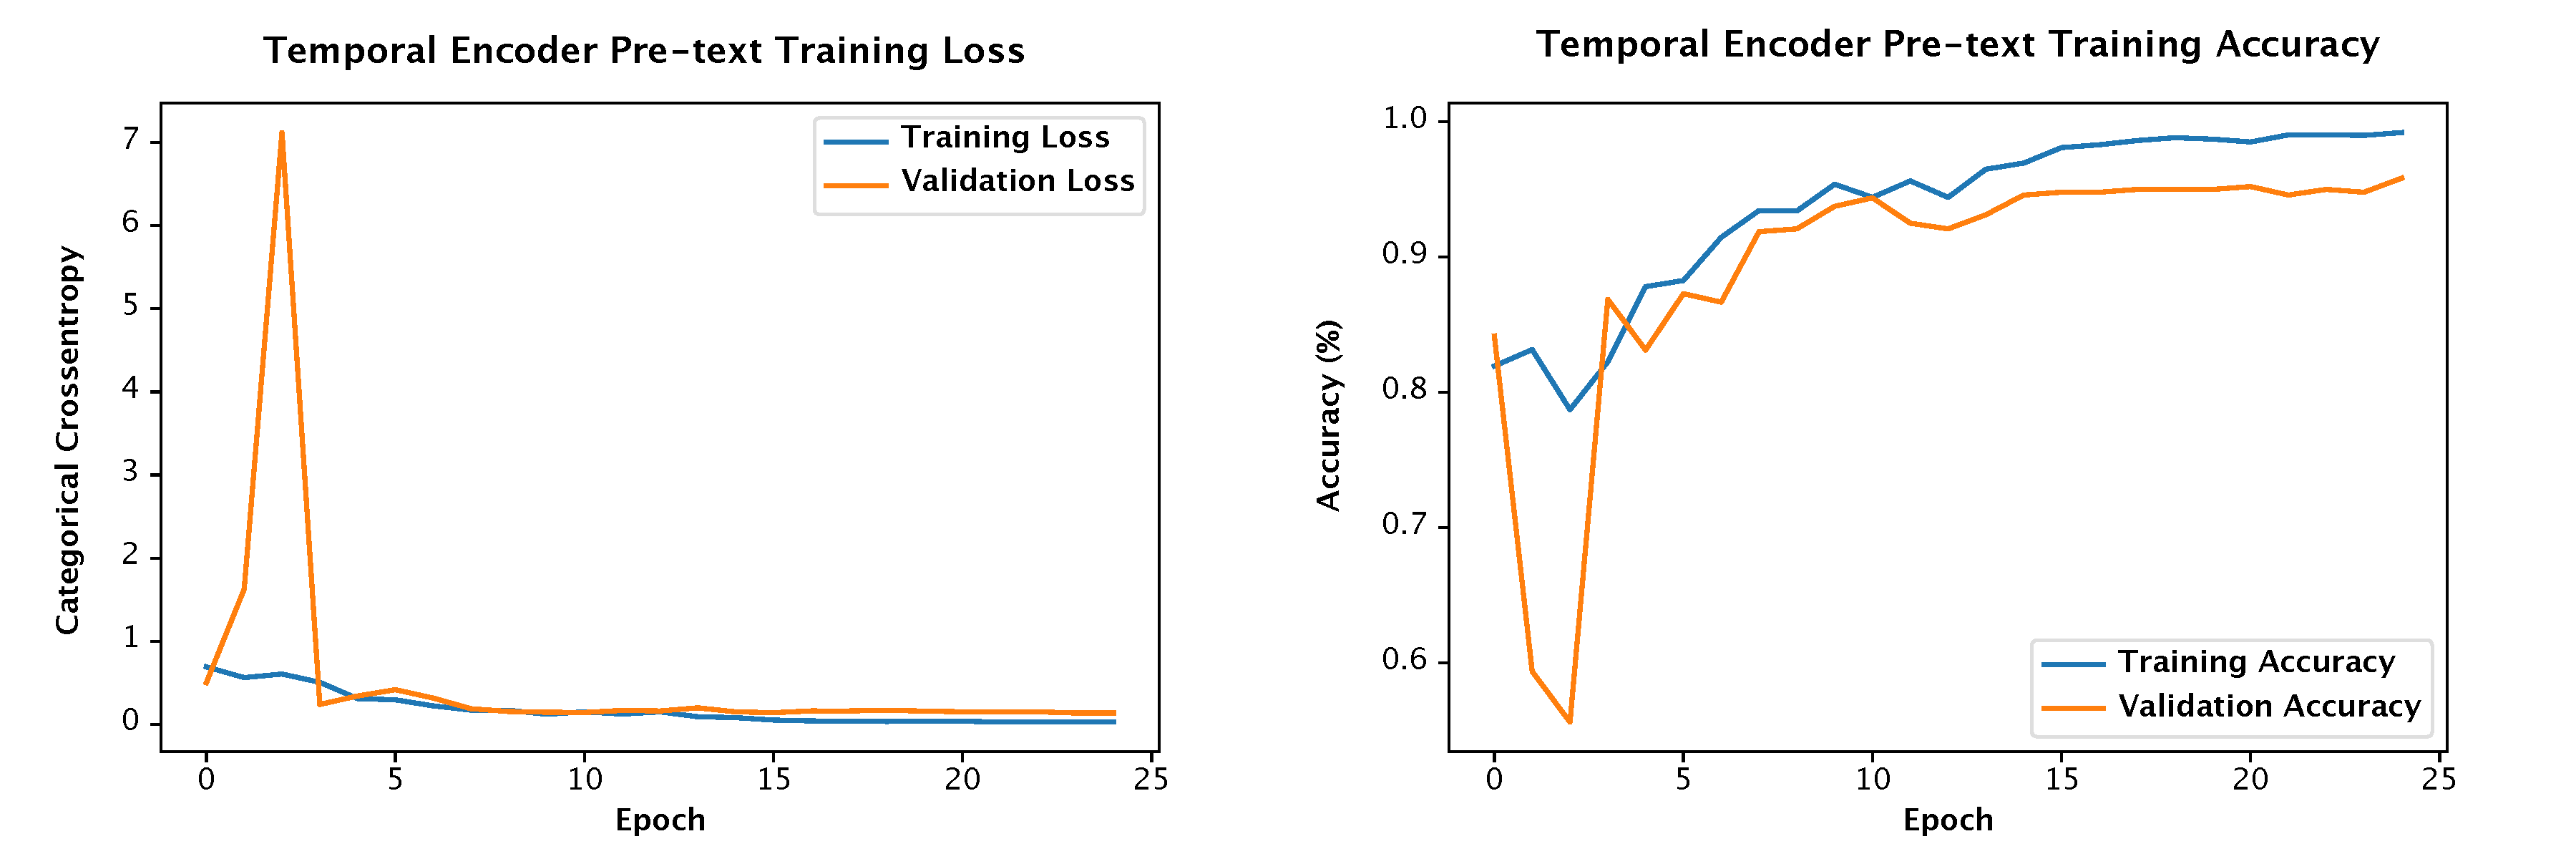
\includegraphics[width=1\textwidth]{HealNet/Fig_4.pdf}
    \caption{Training and validation loss and accuracy for the task of predicting positive or negative temporal pairs.}
    \label{fig:training-curves}
\end{figure}

\subsubsection{Wound Healing Clustering Evaluation}
We performed two-dimensional PCA to visualize the clusters and their centroids. We can observe in Fig. \ref{fig:pca} that our clusters are mostly close together, especially in the later stages. Given that wound progression is slowly evolving and the time step between observations is 1 day, this closeness and some overlap are expected. We can also observe how the hemostasis cluster contains the highest spread. This is likely because this cluster mostly contains day 0 images, where the wound bed is uncovered and artificially illuminated, and day 1 images, where the wound bed is no longer artificially illuminated and is covered with a protective plastic film, leading to some distance between the embeddings. Due to the noisy nature of the dataset, some spread is also expected.

\begin{figure}[h!]
    \centering
    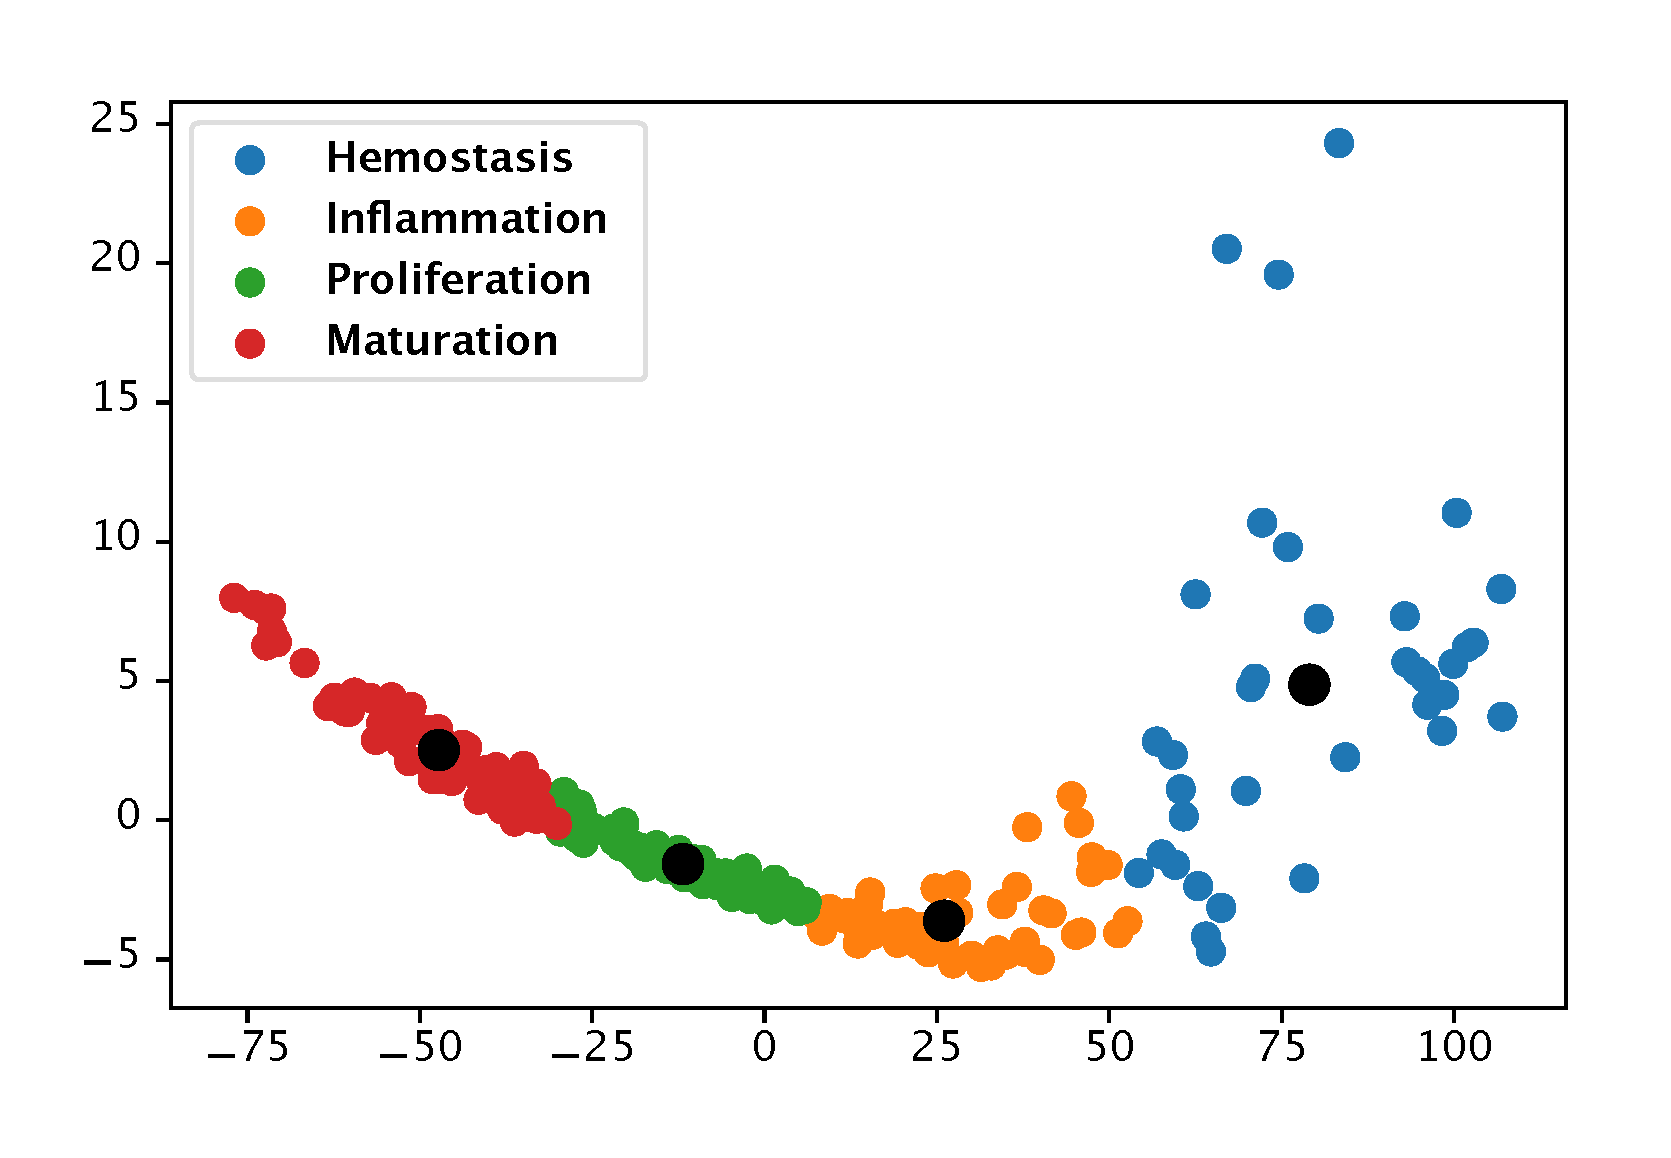
\includegraphics[width=1\textwidth]{HealNet/Fig_5.pdf}
    \caption{K-means ($k = 4$) cluster visualization with centroids using 2-dimensional PCA.}
    \label{fig:pca}
\end{figure}

To further evaluate the quality of the clusters, we examined the images in each cluster (separately for young and aged mice)quartiles. The median wound age (in days) and first and third quartile of wound age are calculated for each cluster. As can be seen from Fig. \ref{fig:stage}, images in each of the clusters contain visual cues for hemostasis (fresh and clearly defined wound-edge), inflammation (swelling of the wound edge, wet and shiny appearance), proliferation (dry and matte appearance with rough and uneven texture), and maturation (complete or near-complete wound closure). In addition, there is a clear temporal progression in the median wound day age that also differentiates our clusters. It would be interesting to note that a difference in wound healing rates between young and aged mice is evident in the first, second, and third quantiles of each cohort. Previous work on this dataset \cite{carrion2021automatic} also reported a similar divergence in wound-size progression between young and aged mice, consistent with these results. These two aspects are used in relating each cluster to a matching heal-stage. To validate these assignments, a blind survey of 5 human non-experts was conducted, in which we found a top-1 agreement of over 80\% between the self-supervised and human labels. Table \ref{tab:table1} presents detailed statistics on the temporal distribution of clusters, and Table \ref{tab:table2} reports human annotator agreement per data split.

\begin{figure}[t!]
    \centering
    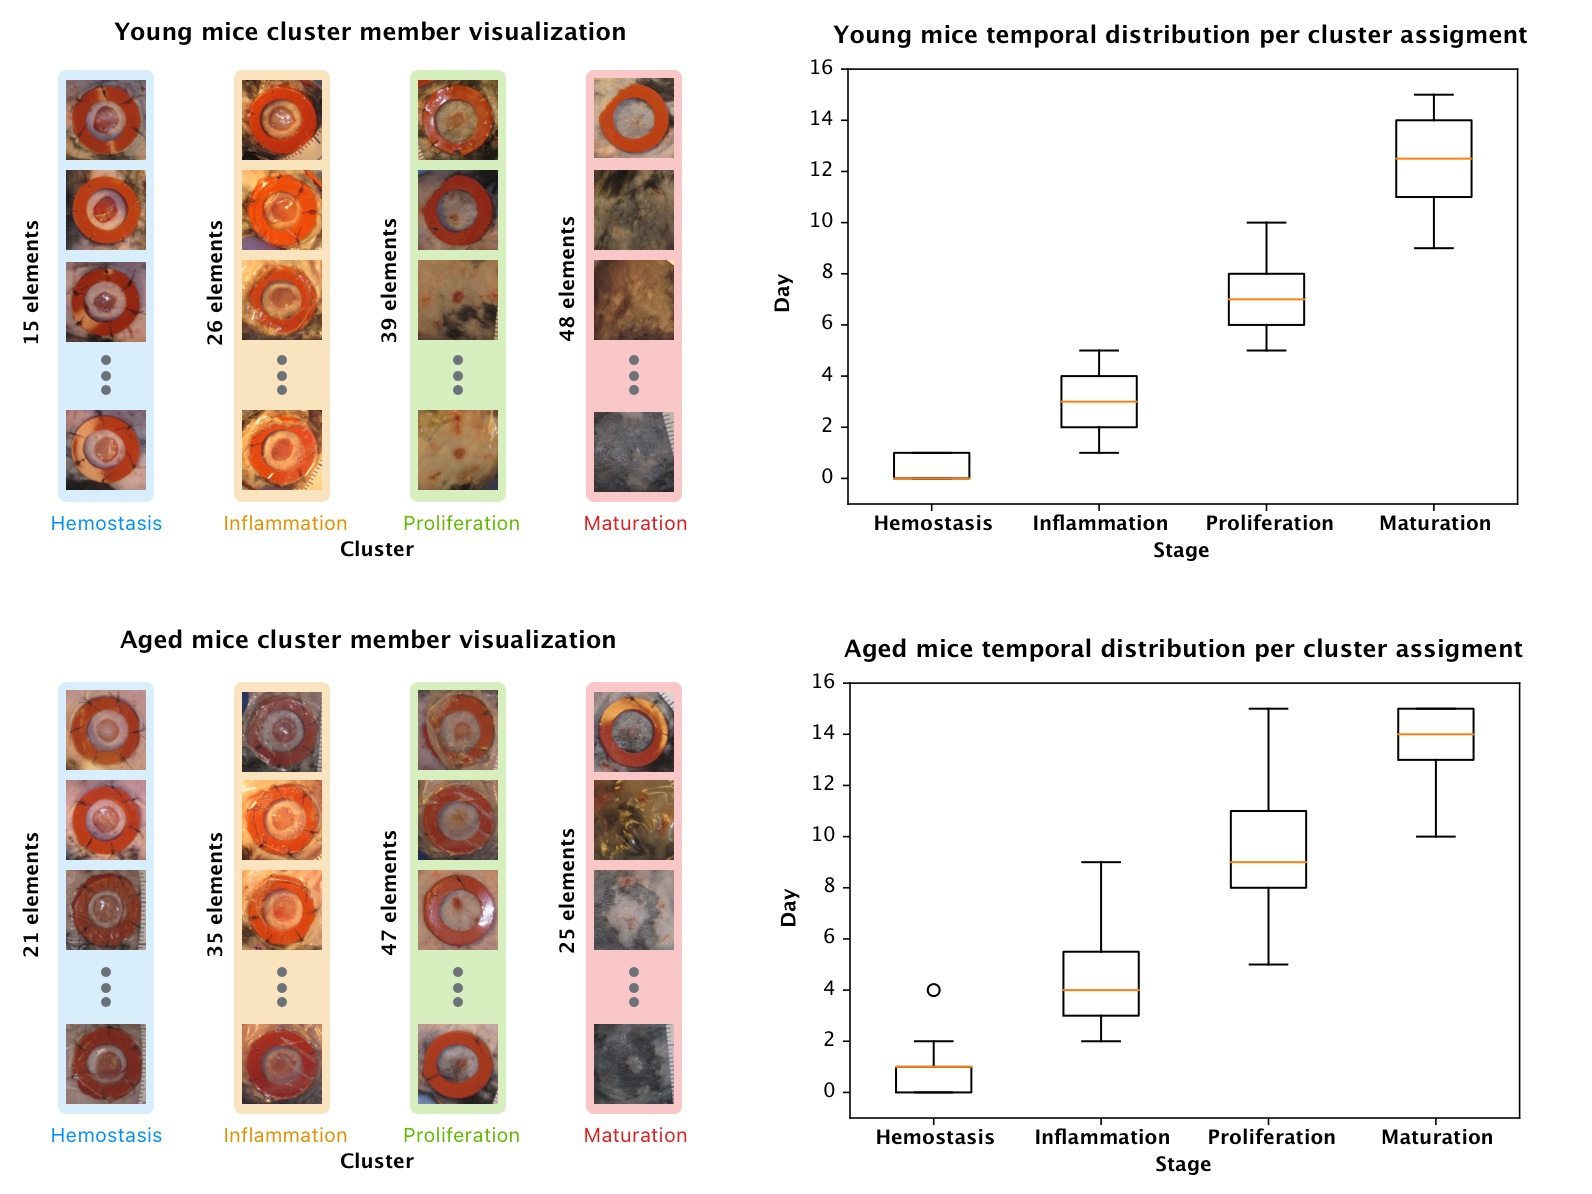
\includegraphics[width=1\textwidth]{HealNet/Fig_6.jpg}
    \caption{\textbf{(left)} Cluster member examples split between young and aged mice and \textbf{(right)} Temporal distribution box plots. Note: We show the original, uncropped images here to verify that the medical red rings (splints) have not biased the cluster members.} We align the cluster groups with a healing stage according to two metrics: visual appearances and wound age distribution metrics.
    \label{fig:stage}
\end{figure}

% \begin{table}[h!]
% \centering
% \caption{Cluster group wound-age (experimental days 0 - 15) statistics.}
% \resizebox{0.44\textwidth}{!}{
% \begin{tabular}{||c|c|c|c|c|c||}
%     \hline
%     Age Group & Cluster & Q1 & Median(Q2) & Q3 & Average\\
%     \hline
%     \multirow{4}{*}{Young}&Cluster 1 & 0.0 & 0.0 & 1.0 & 0.5\\
%     & Cluster 2 & 2.0 & 3.0 & 4.0 & 3.0 \\
%     & Cluster 3 & 6.0 & 7.0 & 8.0 & 7.1\\
%     & Cluster 4 & 11.0 & 12.5 & 14.0 & 12.5\\
%     \hline
%     \multirow{4}{*}{Aged}&Cluster 1 & 0.0 & 1.0 & 1.0 & 1.0\\
%     &Cluster 2 & 3.0 & 4.0 & 5.5 & 4.5\\
%     & Cluster 3 & 8.0 & 9.0 & 11.0 & 9.6\\
%     & Cluster 4 & 13.0 & 14.0 & 15.0 & 13.4\\
%     \hline
% \end{tabular}
% }
% \label{tab:table1}
% %\vspace{-10mm}%Put here to reduce too much white space after your table 
% \end{table}

\subsubsection{Wound Stage Classification}
The wound stage classification model is trained until convergence. While this task contains fewer training samples ($15\times$ fewer), the loss curves show that the network is not overfitting, achieves relatively high accuracy on the validation set, and can predict the heal-stage for the training, validation, and test sets (Table \ref{tab:table3}). The accuracy for the wound stage classification task is 95.8\%, 87.5\%, and 90.6\% on training, validation, and test sets, respectively. Finally, we trained an identical architecture as a straightforward CNN Classifier (without the pre-text task), using the collected human survey labels to compare performance. Under these conditions, the network achieved lower accuracies of 83.3\%, 81.3\%, and 78.1\% on the training, validation, and test sets, respectively. Table \ref{tab:table3} summarizes the loss and accuracy scores described above.

\begin{table}[h]
\centering
\caption{Human annotator vs. automatic pseudo-label agreement.}
\resizebox{0.22\textwidth}{!}{
\begin{tabular}{||c|c||}
    \hline
    Data Split & Agreement (\%)\\
    \hline
    Train & 80.7 \\
    \hline
    Validation & 71.9 \\
    \hline
    Test & 87.5 \\
    \hline
    Overall & 80.5 \\
    \hline
\end{tabular}
}
\label{tab:table2}
%\vspace{-10mm}%Put here to reduce too much white space after your table 
\end{table}

\begin{figure}[h]
    \centering
    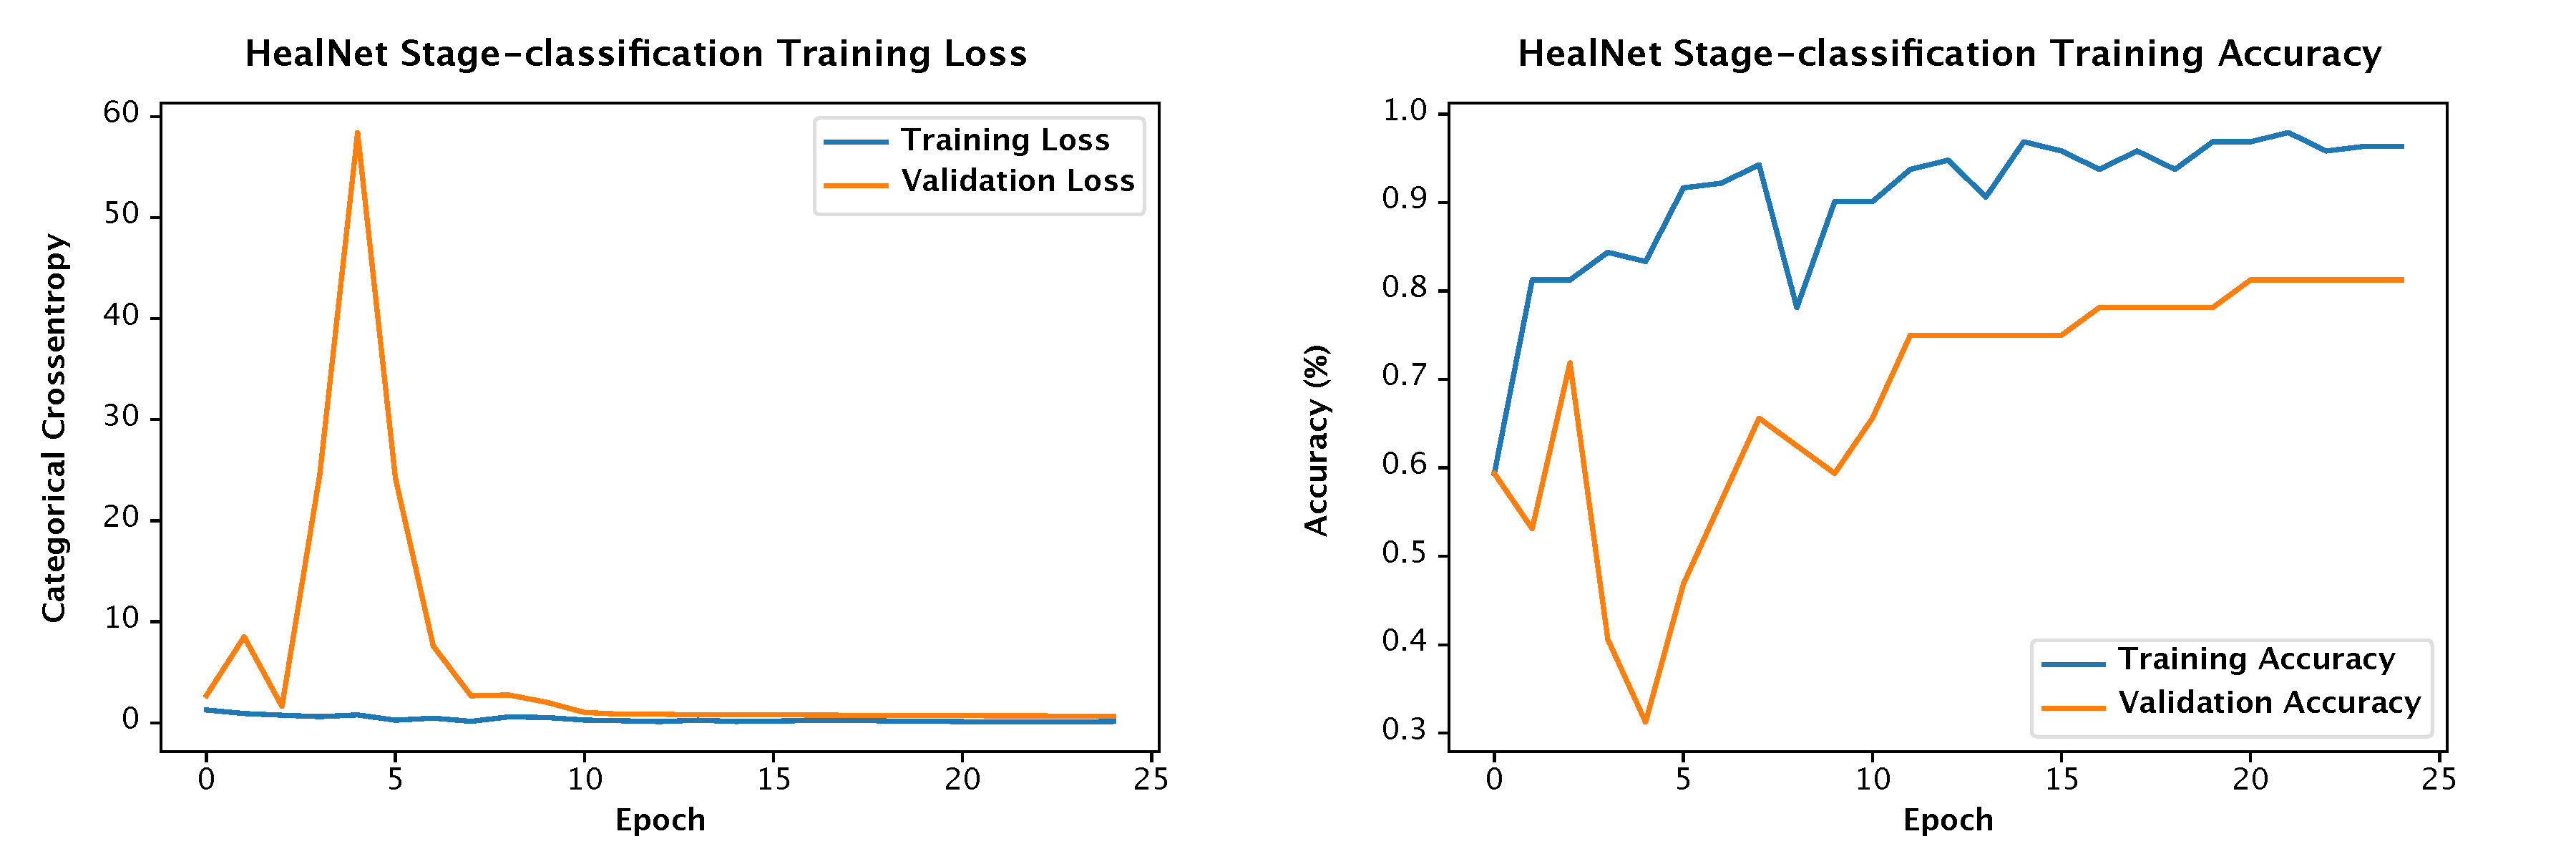
\includegraphics[width=1\textwidth]{HealNet/Fig_7.pdf}
    \caption{Training and validation loss and accuracy for the task of predicting the healing stage.}
    \label{fig:classification-results}
\end{figure}
% %\vspace{-0.5 in}

\begin{table}[h]
\centering
\caption{Performance metrics across both temporal coherency and wound stage classification tasks for training, validation, and test sets.}
\resizebox{0.58\textwidth}{!}{
\begin{tabular}{||c|c|c|c||}
    \hline
    Task & Train Acc. & Val. Acc. & Test Acc.\\
    \hline
    Supervised Classifier (baseline) & 83.3\% & 81.3\% & 78.1\% \\
    \hline
    Temporal Coherency (pre-text) & 97.2\% & 95.0\% & 97.7\% \\
    Wound Stage Classification (downstream) & \textbf{95.8\%} & \textbf{87.5\%} & \textbf{90.6\%} \\
    \hline
\end{tabular}
}
\label{tab:table3}
%\vspace{-10mm}%Put here to reduce too much white space after your table 
\end{table}
% %\vspace{-0.5 in}

\subsubsection{Computational Performance}
The average run-time for pre-text training was about 10 minutes or ~25 seconds per epoch ($\sim$125ms/step) over 25 epochs. The average runtime for the downstream task was about 1 min, or ~2.5s per epoch ($\sim$150ms/step), over 25 epochs. This faster train time is due to the smaller downstream dataset. Memory footprint did not exceed 16GB on either system memory or GPU memory after multiple runs. Inference time is equal to about 17 images per second.


% Paper 2
\chapter{Representation Learning, Fairness and Efficiency}\label{section:fedd}

HealNet (Chapter~\ref{section:healnet}) showed that label-free representation learning is feasible when the data carry reliable temporal structure. Most clinical dermatology, however, is single-image: a patient comes in once with a lesion and leaves once with a diagnosis, so the temporal pretext signal is unavailable. HealNet was also restricted to a small cohort of mice and offered no skin-tone-stratified evaluation. This chapter generalizes representation learning to the single-image setting by treating the internal features of a frozen denoising-diffusion backbone as the encoder, and adds the first explicit fairness evaluation of the dissertation: skin-tone-stratified segmentation and malignancy classification on the Diverse Dermatology Images benchmark with biopsy-confirmed, dermatologist-verified Fitzpatrick labels.

\section{FEDD - Fair, Efficient, and Diverse Diffusion-based Lesion Segmentation and Malignancy Classification}\label{section:fedd_abs}
Skin diseases affect millions of people worldwide, across all ethnicities. Increasing diagnosis accessibility requires fair and accurate segmentation and classification of dermatology images. However, the scarcity of annotated medical images, especially for rare diseases and underrepresented skin tones, poses a challenge to the development of fair and accurate models. In this study, we introduce a Fair, Efficient, and Diverse Diffusion-based framework for skin lesion segmentation and malignancy classification. FEDD leverages semantically meaningful feature embeddings learned through a denoising diffusion probabilistic backbone and processes them via linear probes to achieve state-of-the-art performance on DDI. We achieve improvements in intersection over union of 0.18, 0.13, 0.06, and 0.07 when using only 5\%, 10\%, 15\%, and 20\% labeled samples, respectively. Additionally, FEDD trained on 10\% of DDI achieves a malignancy classification accuracy of 81\%, 14\% higher than the state-of-the-art. We demonstrate high efficiency in data-constrained scenarios while delivering fair performance across diverse skin tones and rare malignancy conditions.


\subsection{Background and Related Work}\label{sec:intro}
Skin diseases are a major public health concern that impacts millions of people worldwide. The first step towards diagnosis and treatment of skin diseases often involves visual inspection and analysis of the lesion by dermatologists or other medical experts. However, this process is often subjective, time-consuming, costly, and inaccessible for many people, especially in low-resource communities or remote areas. It is estimated that around 3 billion people lack adequate access to dermatological care \cite{coustasse_2019_use}. In the United States, only about one in three patients with skin disease is evaluated by a dermatologist; their average wait time exceeds 38 days, and this care represents a cost of \$75 billion to the healthcare system \cite{a2016_burden,tsang_2006_even}. Therefore, there is a growing need for automated methods to assist dermatologists, especially those in low-resource environments, in accurately and efficiently attending to skin lesions.

Skin lesion semantic segmentation and malignancy classification are essential for providing accurate and explainable diagnostic information for patients with skin diseases, and, recently, AI systems have led the state-of-the-art for these tasks. However, these systems are commonly based on data and training methods that are prone to racial biases \cite{daneshjou_2022_disparities,owens_2020_those,chen_2021_ethical}. Some of the main challenges facing AI systems that can lead to bias are:
\begin{itemize}
  \item \textbf{Data scarcity:} Annotated medical images are often scarce and expensive to obtain due to privacy issues, cost, and expert availability. This limits the amount of data available for training DL models, which may lead to overfitting, especially in medical contexts, as shown in \cite{razzak_2017_deep}.
  \item \textbf{Class imbalance:} The distribution of different types of skin lesions is often imbalanced in real-world datasets. For example, melanoma cases may be rarer than basal cell carcinoma cases; this could then be exacerbated by datasets that are primarily sourced from light-skinned populations \cite{groh_2021_evaluating}. This class imbalance can introduce biases in modeling.
  \item \textbf{Data diversity:} The appearance and morphology of skin lesions can vary across different individuals due to factors such as age, gender, and ethnicity \cite{adelekun_2020_skin}. A dataset can be large but not necessarily diverse. This lack of diversity in the data may lead to poor generalization \cite{daneshjou_2022_disparities}.
  \item \textbf{Base models:} Some recent works on dermatology images stem from transfer-learning models designed for ImageNet \cite{deng_2009_imagenet}, which may be overly large for smaller dermatologic datasets \cite{esteva_2017_dermatologistlevel,han_2020_augmented}. Tuning these massive encoders could lead to overfitting.
  \item \textbf{Lack of diverse studies:} A recent review of 70 dermatological AI studies between 2015 and 2020 found that only 17 studies included ethnicity descriptors, and only 7 included skin tone descriptors \cite{daneshjou_2021_lack}. This could lead to under-specification of model performance for different ethnicities.
\end{itemize}

DDPMs have been introduced \cite{ho_2020_denoising} as a new form of generative modeling. DDPMs have achieved state-of-the-art performance in image synthesis \cite{dhariwal_2021_diffusion} and are effectively applied in colorization \cite{song_2021_scorebased}, super-resolution \cite{saharia_2022_image}, segmentation \cite{baranchuk_2022_labelefficient}, and other tasks. In the medical domain, recent work has presented results for DDPM-based anomaly detection \cite{wolleb_2022_diffusion} and segmentation \cite{wu_2023_medsegdiffv2}, but these are limited to MRI, CT, and ultrasonography, not natural smartphone-captured images of dermatology conditions. To our knowledge, none have explored segmentation and malignancy classification in this context from DDPM-based embeddings without re-training and evaluated performance on diverse dermatology images.

We introduce the FEDD framework, a denoising diffusion-based approach trained on small, skin tone-balanced DDI \cite{daneshjou_2022_disparities} subsets for skin lesion segmentation and malignancy classification that outperforms state-of-the-art across a diverse spectrum of skin tones and malignancy conditions with very few training examples. FEDD leverages the highly semantically meaningful feature embeddings learned by DDPMs for image synthesis. Finally, linear probes predict per-pixel class or per-image malignancy, achieving state-of-the-art performance on the DDI dataset without fine-tuning the encoder.

\subsection{Dataset}
The most commonly used dataset for training and evaluating fairness in dermatology AI is Fitzpatrick17k \cite{groh_2021_evaluating,abid_2022_meaningfully,du_2023_fairdisco}, thanks to its large size of nearly 17,000 images. However, it contains a significant skin tone imbalance (3.6 times more light than dark skin-toned samples) and greater than 30\% disease label noise \cite{groh_2021_evaluating}. Further, the samples are not biopsied, and visual inspection alone can be an unreliable means of diagnosis without histopathological information \cite{daneshjou_2022_checklist}. Recently, DDI \cite{daneshjou_2022_disparities} was published as a dermatological image dataset with Fitzpatrick-scale \cite{fitzpatrick_1988_the} scores for all images, classifying them as light (I-II), medium (III-IV), or dark (V-VI) in skin tone. At a lower skin-tone resolution (3-point instead of 6-point), these labels are reviewed by two board-certified dermatologists. It also includes a mix of rare and common benign and malignant skin conditions, all of which are confirmed via biopsy. The dataset contains visually ambiguous lesions that would be difficult to diagnose visually but represent the kinds of lesions seen in clinical practice. DDI is somewhat balanced between skin tones, with about 16\% more information for medium skin tones; however, it is not balanced between malignant and benign classes. In total, the dataset contains 656 samples. Details and distribution of diagnosis are shown in Fig. \ref{fig:DDI}.

\begin{figure*}[t!]
    \centering
    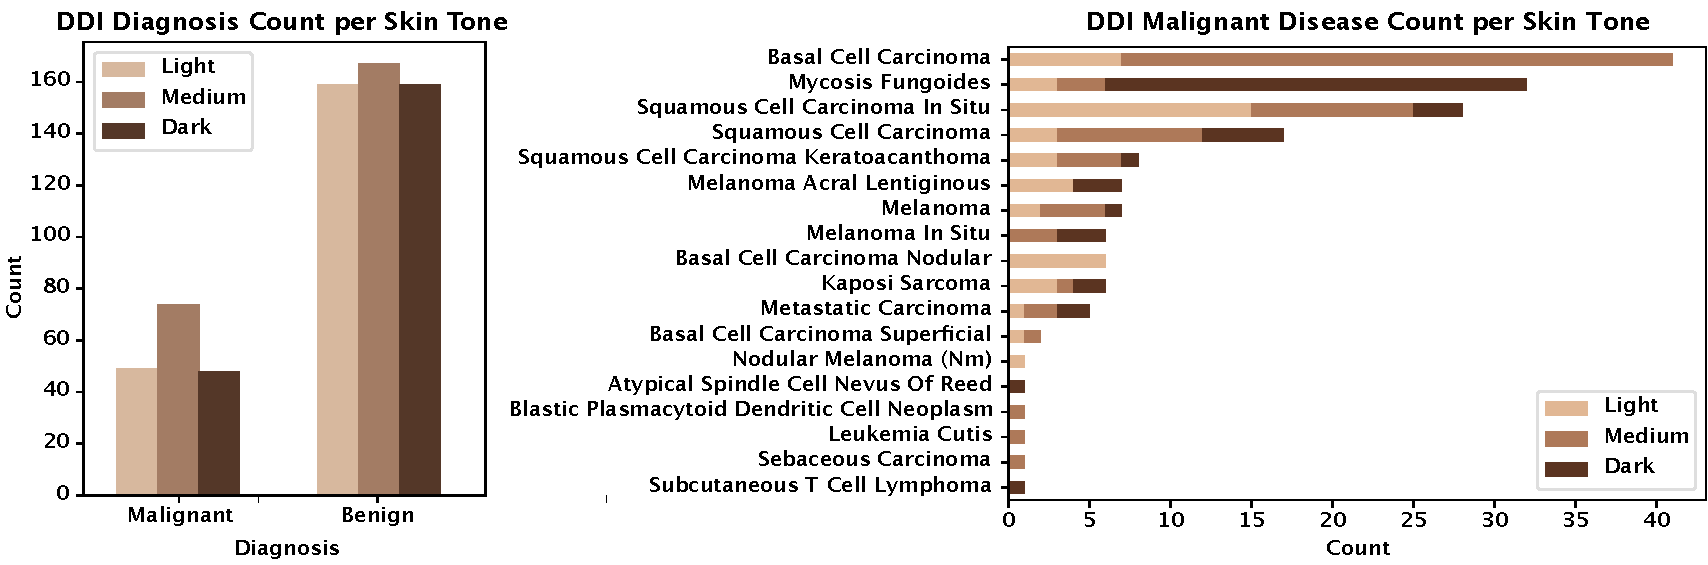
\includegraphics[width=1\textwidth]{FEDD/Fig_1.pdf}
    \caption{The disease count per skin tone (left) shows a smaller amount of malignancy data in DDI but otherwise mostly balanced between light and dark skin tones. The distribution of malignant illnesses (right) shows high diversity and thus the morphological variation of lesions in DDI.}
    \label{fig:DDI}
    %\vspace{-2mm}%Put here to reduce too much white space
\end{figure*}

\begin{figure*}[t!]
    \centering
    \includegraphics[width=1\textwidth]{FEDD/Fig_2.pdf}
    \caption{Ground truth segmentation samples. We color-code lesions as red, skin as green, markings as purple, and rulers as blue. Backgrounds are left to be transparent.}
    \label{fig:DDI_annots}
    %\vspace{-5mm}%Put here to reduce too much white space
\end{figure*}

We draw 4 balanced subsets of DDI for training, each representing approximately 5\% (10 samples per skin tone), 10\% (20 samples per skin tone), 15\% (30 samples per skin tone), and 20\% (40 samples per skin tone) of DDI. The smaller training sets are subsets of the larger ones, this is to say $5\% \subseteq 10\% \subseteq 15\% \subseteq 20\% \subseteq$ DDI. For classification, we draw validation and test sets, each containing 30 samples (10 samples per skin tone). Further, we test model checkpoints trained on each DDI subset on all remaining DDI images (476 samples), and the accuracy results from this larger test set are reported in the paper text and in Table 3 of the supplementary materials. For segmentation, we test on 198 additionally annotated samples.

%The testing set contains all remaining DDI samples for classification and 198 images for segmentation. The test sets are skin-tone unbalanced, as is expected in clinical settings. Validation and test sets are disjoint from the training splits and from each other.

This is due to DDI's inclusion of disease labels suitable for malignancy classification. For segmentation, however, samples need to be semantically labeled, and some may be difficult to annotate correctly, leading to their discard; for example, if the target lesion is ambiguous, blurry, partially visible, or occluded. We annotated the dataset, and all masks underwent a secondary quality review. We define 5 classes: lesion, skin, marker, ruler, and background. We opted to label these classes, as many images include a ruler or markings to denote the lesion of focus. Visualizations of our ground truth labels are shown in Fig. \ref{fig:DDI_annots}. Details on the annotation protocol, including skip criteria, can be found in the supplementary materials. We release our annotated DDI images (a total of 378) as part of our contributions.

\subsubsection{Annotation Process}
As mentioned previously, we draw 4 balanced subsets of DDI for training, each representing approximately 5\% (10 samples per skin tone), 10\% (20 samples per skin tone), 15\% (30 samples per skin tone), and 20\% (40 samples per skin tone) of DDI. The smaller training sets are subsets of the larger ones, this is to say $5\% \subseteq 10\% \subseteq 15\% \subseteq 20\% \subseteq$ DDI. For classification, we draw validation and test sets, each containing 30 samples (10 samples per skin tone). Further, we test model checkpoints trained on each DDI subset on all remaining DDI images (476 samples), and the accuracy results from this larger test set are reported in the paper text and in the supplementary materials Table 3. For segmentation, we test on 198 additionally annotated samples (59 light, 80 medium, and 59 dark in skin tone). These larger test sets are skin-tone unbalanced, as expected in clinical settings. All validation and testing sets are disjoint from the training splits and from each other.

For malignancy classification, DDI includes disease labels. For segmentation, sample images need to be semantically labeled, and some may be difficult to annotate; the annotation protocol is as follows:

\begin{enumerate}
  \item Lesion is segmented following the boundary at which the skin transitions from healthy to unhealthy appearance.
  \item Markings or rulers are segmented in their visible totality.
  \item Non-lesion, or normal skin, is segmented.
\end{enumerate}

This denotes our segmentation masks, which cover 5 different classes: lesion, skin, marker, ruler, and background. We opted to label these classes, as many images include a ruler and markings to denote the lesion of focus. All other potentially present objects, such as clothing, were designated as background.

Not all images were suitable for labeling, as DDI images may not have been collected with computer vision in mind and consequently were skipped. The following criteria will trigger a skip: 

\begin{enumerate}
  \item Lesion is occluded.
  \item Lesion is significantly blurry.
  \item Lesion is only partially visible.
  \item Target lesion is ambiguous (no lesions marked when multiple are present or multiple are marked in a single image).
  \item Lesion is on or near the scalp (hair is not a labeled target and is time-consuming to annotate).
\end{enumerate}

Examples of images that triggered a skip can be found on DDI sample id 25, 55, and 161. The total number of annotated images that passed our annotation criteria and secondary review is 378. We have released this annotation work on our GitHub, linked in the abstract. Table \ref{tab:DDI_Subsets} describes our training subsets of the Diverse Dermatology Images dataset.

\begin{table}[h]
\centering
\caption{The distribution of training data per sub-set of DDI.}
\resizebox{1\textwidth}{!}{
\begin{tabular}{||c|c|c|c|c||}
    \hline
    DDI Subset & Total Samples & Samples per Skin Tone & Malignant Samples per Skin Tone & Benign Samples per Skin Tone\\
    \hline
    5\% & 30 & 10 & 5 & 5 \\
    \hline
    10\% & 60 & 20 & 10 & 10 \\
    \hline
    15\% & 90 & 30 & 15 & 15 \\
    \hline
    20\% & 120 & 40 & 20 & 20 \\
    \hline
\end{tabular}
}
\label{tab:DDI_Subsets}
%\vspace{-10mm}%Put here to reduce too much white space after your table 
\end{table}

\subsection{Method}
The UNet architecture was introduced for diffusion \cite{ho_2020_denoising} and has been shown to improve generative performance \cite{jolicoeurmartineau_2020_adversarial} over other denoising score-matching architectures. Recent work \cite{dhariwal_2021_diffusion} has extensively ablated the diffusion UNet architecture by increasing depth while reducing the width, increasing the number of attention heads, and applying it at different resolutions, applying BigGAN \cite{brock_2018_large} residual blocks, and introducing AdaGN for injecting timestep and class embedding onto residual blocks, obtaining state-of-the-art for image synthesis. From this work, we designate the unconditional image generation model as our backbone and freeze its weights. This network is an ImageNet-trained DDPM with $256\times256$ input and output resolution.
\begin{figure*}[t!]
    \centering
    \includegraphics[width=1\textwidth]{FEDD/Fig_3.pdf}
    \caption{Image noise is added according to the diffusion noise schedule for the selected timestep. The DDPM processes the image, and feature embeddings are obtained from the desired block levels. Embeddings are concatenated and either up-sampled for segmentation or down-sampled for classification. Finally, Multi-Layer Perceptrons (MLPs) predict per-pixel semantic classes or whole-image malignancy.}
    \label{fig:FEDD}
    %\vspace{-5mm}%Put here to reduce too much white space
\end{figure*}

\subsubsection{Lesion, Marker, Ruler, Skin, and Background Segmentation}
We obtain image encodings from blocks on the decoder side of the DDPM-UNet architecture, then apply bilinear up-sampling to a target output resolution ($256\times256$ in this case) and concatenate them before feeding them to MLPs for per-pixel classification, following \cite{baranchuk_2022_labelefficient}. However, we use fewer blocks, a single time step, and 5 MLPs. This is to avoid overfitting, and because results from \cite{baranchuk_2022_labelefficient} show that different blocks at different timesteps perform differently depending on the target data. To identify which blocks are most promising for dermatology images, we obtain feature encodings from different blocks and perform K-Means clustering, as shown in the supplementary materials. We selected the blocks that clustered semantically meaningful areas (e.g., lesion, skin, and ruler). We identify blocks 6 and 8 at timestep 100 as the most promising and use this setup for the rest of our segmentation experiments.

\subsubsection{Malignancy Classification}
For classification, we downsample block encodings using a combination of 2D and 1D max pooling operations until the feature vectors are 1D and 512-dimensional. We note that the total number of pooling operations varies across blocks: deeper blocks are smaller and have more channels, whereas shallower blocks are larger and have fewer channels. The vectors are then passed to a 3-layer MLP with sizes 64, 32, and 1. We include batch normalization and dropout between layers at 50\% and 25\%, respectively. This classification network is trained to predict the malignancy of the input image based on the downsampled feature vector. A summary of our approach is shown in Fig. \ref{fig:FEDD}.

\subsubsection{Computational Setup}
All code involving this study was written in Python v3.7.12. The packages used for training and inference were the latest available stable versions of deep learning frameworks PyTorch v1.13, Keras v2.8, and TensorFlow v2.8. Additional packages used for numerical processing, plotting, and visualization were Pandas v1.3.5, NumPy v1.21.5, scikit-learn v1.0.2, PIL v7.1.2, and Matplotlib v3.5.1. The hardware used was a Google Colab instance running a quad-core Intel Xeon CPU at 2.3 GHz, 80GB of RAM, and an NVIDIA A100 GPU with 40GB of vRAM.

\subsubsection{Additional Hyper-parameters and Experimental Setup}
Additional hyperparameters used were batch sizes of 30, 60, 90, and 120 for 5, 10, 15, and 20\% of DDI, respectively. These were selected as they allowed all subset data to be processed in a single batch. For testing and validation, a batch size of 30 was used. The Adam optimizer was used, along with weight decay equal to $0.00001$. The loss function is Binary Cross-Entropy. The MLPs were trained over 500 epochs with early stopping monitoring the validation loss. Most runs were early-stopped at or before 100 epochs.

\subsection{Results and Discussion}
\label{sec:fedd_results}
\subsubsection{Lesion, Marker, Ruler, Skin, and Background Segmentation}
Our segmentation results are evaluated by Intersection over Union (IoU) performance and are compared against other architectures pre-trained on ImageNet: DenseNet121 \cite{huang_2016_densely}, VGG16 \cite{simonyan_2014_very}, ResNet50 \cite{he_2015_deep}, and two other smaller networks, EfficientNetB0 \cite{tan_2019_efficientnet} and MobileNetV2 \cite{sandler_2018_mobilenetv2}. These architectures are configured as UNets and tasked with segmenting the input images. We observe that FEDD outperforms all other architectures across all DDI subsets on our validation and test sets. Importantly, other architectures (particularly smaller networks) close the performance gap as training data increases, showing that FEDD's efficiency is most pronounced in very small data scenarios.

We further compare FEDD's IoU performance on images with light and dark skin tones to demonstrate algorithmic fairness. We note that all architectures show similar performance for both skin tones, suggesting that our balanced data subsets play a larger role in fairness than the choice of neural network. Finally, we plot the test set performance when considering only the lesion class split between light and dark tones. We find that FEDD's performance is significantly better at segmenting lesion classes than other architectures. We believe this is because the greater morphological variation among different skin lesions makes them harder to learn than other, more consistent targets like the ruler. Since DDI encompasses a diverse range of skin conditions, FEDD's efficiency is particularly useful for high-quality lesion segmentation in this morphologically variable class. These results are shown in Fig. \ref{fig:IoUs}.

\begin{figure*}[t!]
    \centering
    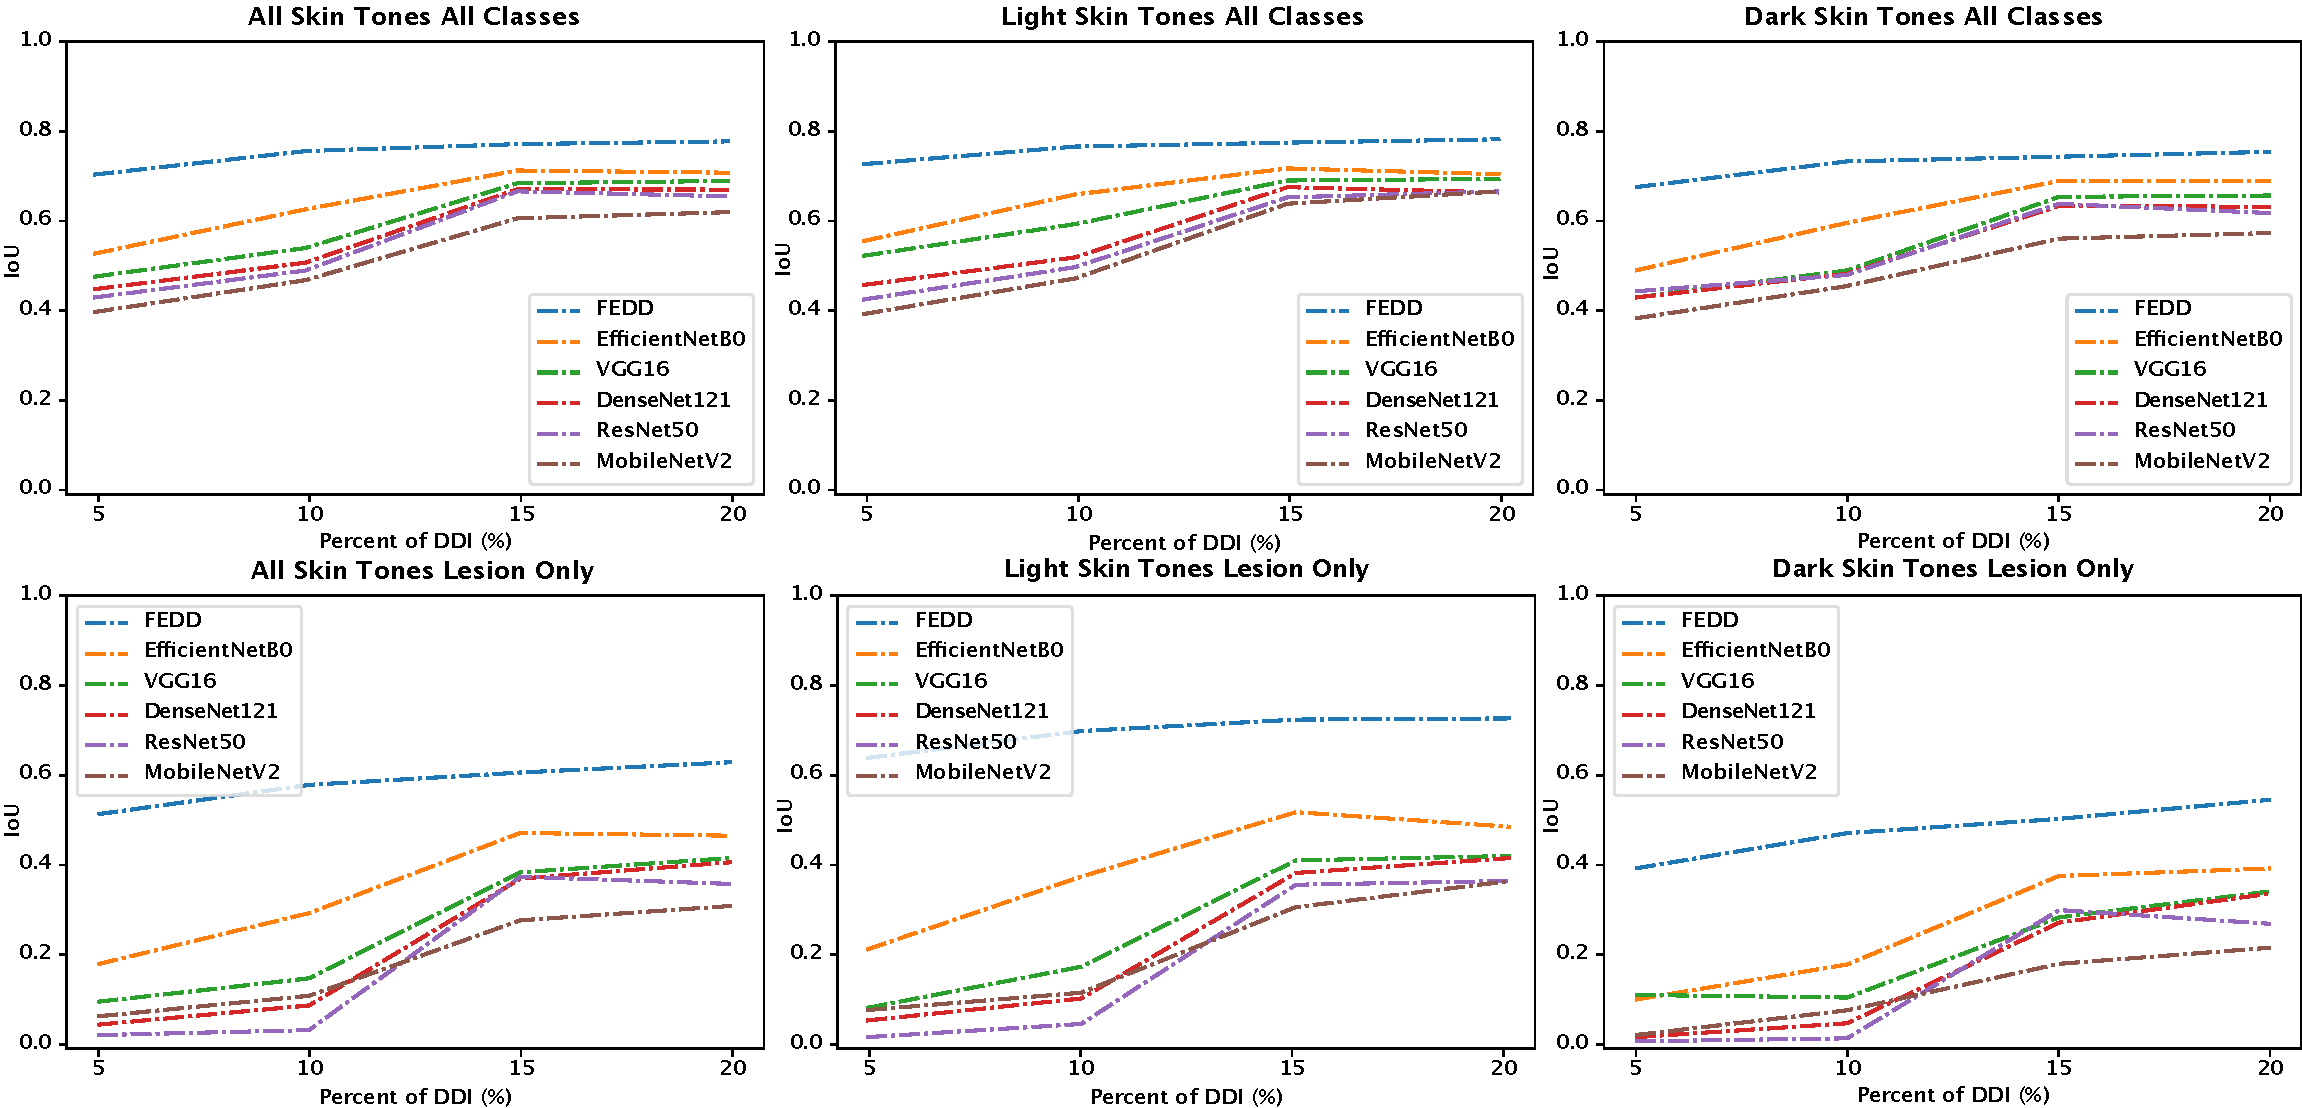
\includegraphics[width=1\textwidth]{FEDD/Fig_4.pdf}
    \caption{\textbf{Top Row}: The test IoU score for all segmentation classes for all, light, and dark skin tones (left-to-right). \textbf{Bottom Row}: The test IoU score for the lesion segment for all, light, and dark skin tones (left-to-right).}
    \label{fig:IoUs}
    %\vspace{-5mm}%Put here to reduce too much white space
\end{figure*}

In Fig. \ref{fig:Segs}, we visualize predicted segmentation masks between FEDD and the next best IoU-performing architecture, EfficientNetB0. We observe that FEDD achieves significantly better segmentation masks at lower fractions of labeled data across all skin tones. With a larger percentage of labeled data, EfficientNet begins to produce results similar to FEDD, but FEDD produces higher-quality segmentations with fewer segmentation artifacts and false positives. The skin lesions themselves, which vary in size, location, and morphology, are also most accurately segmented by FEDD.

\begin{figure*}[t!]
    \centering
    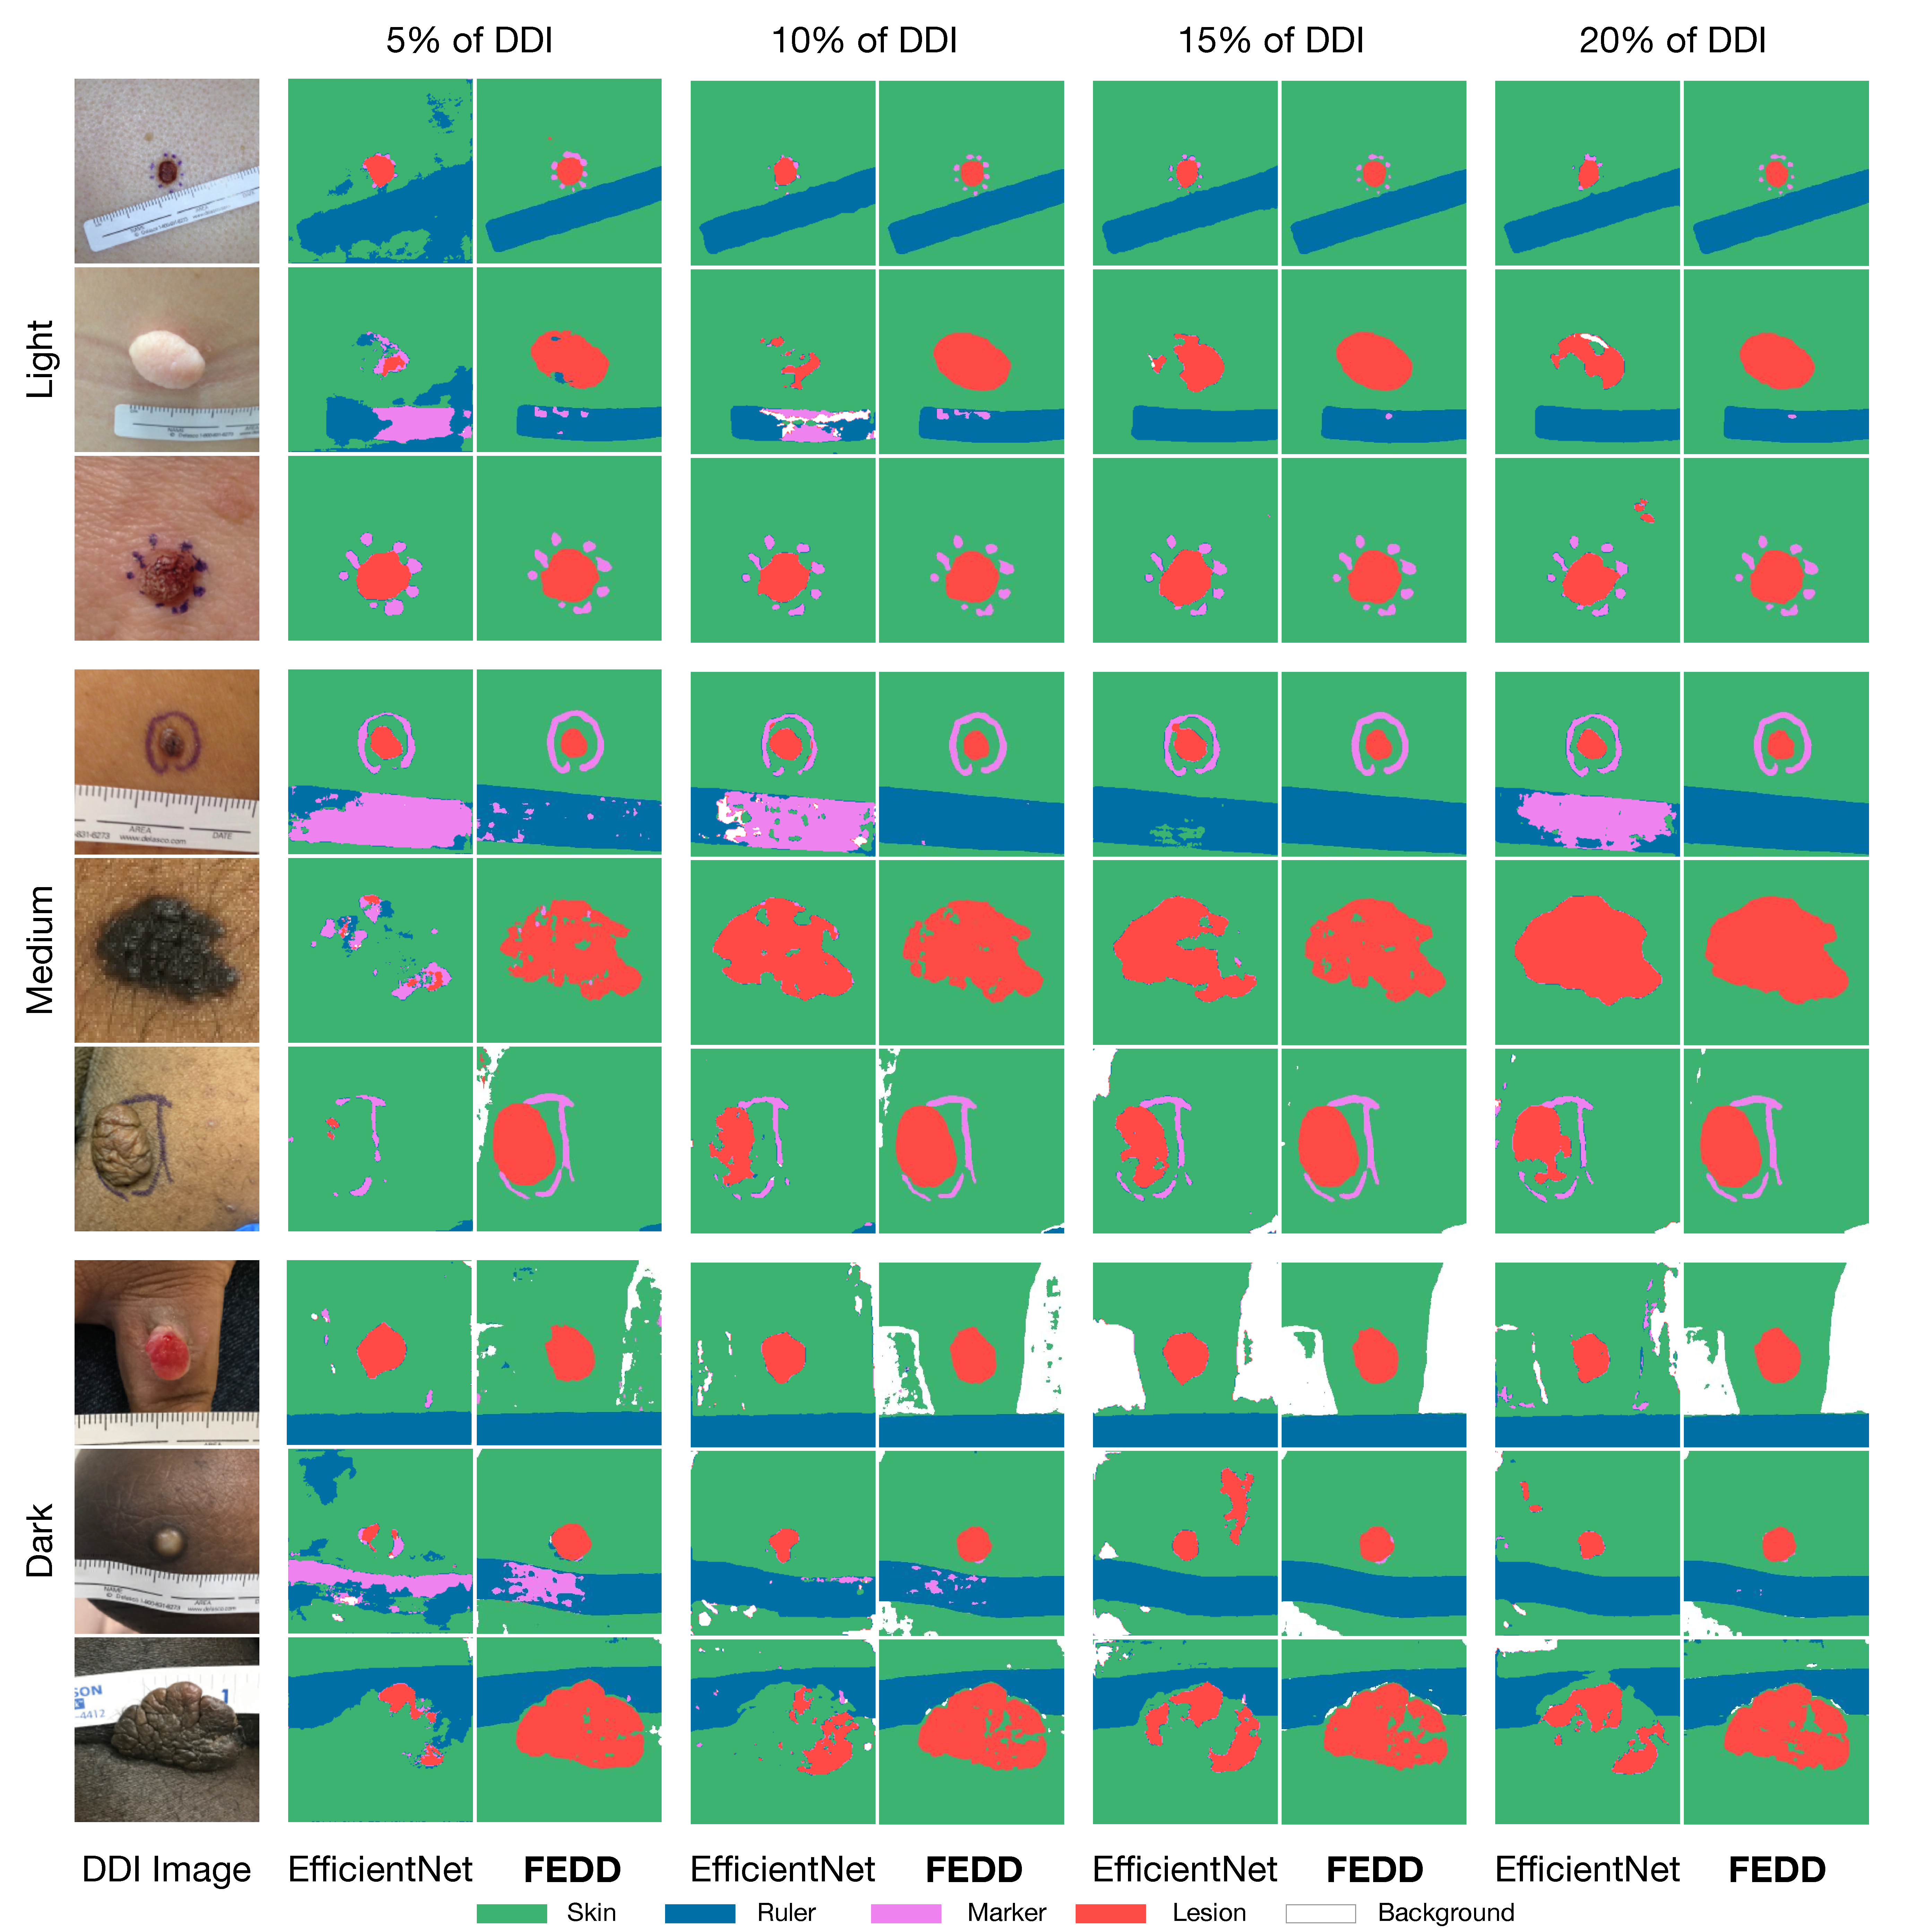
\includegraphics[width=1\textwidth]{FEDD/Fig_10.pdf}
    \caption{Test set segmentation results for FEDD and EfficientNet.}
    \label{fig:Segs}
    %\vspace{-5mm}%Put here to reduce too much white space
\end{figure*}

\subsubsection{Malignancy Classification}
We ablate the performance of each individual block at each timestep in the classification context, as, to the best of our knowledge, this has not been done before. It is also not entirely intuitive which block depth and timestep combination would produce the best representations for classification, or how that performance varies as we introduce more data. We train FEDD's classifier on block embeddings produced between timestep 0 and 1000 of the backward diffusion process. We then record the classifier's accuracy per block, in increments of 50 timesteps. Fig. \ref{fig:Cls_Blocks} describes these results. While noisy, given the small amount of test data, the general pattern is that earlier time steps (later in the reverse diffusion denoising process) yield higher classification accuracy. This is likely due to the quality of the DDPM sample increasing as more noise is removed. Another finding is that as the classifier is shown more data, the shallower blocks begin to perform better. The best-performing blocks are block 4 at 5\% DDI, block 6 at 10\% DDI, block 12 at 15\% DDI, and block 14 at 20\% DDI. We attribute this to the fact that shallower blocks of the UNet decoder capture finer detail of the reconstructed image while deeper blocks capture lower-resolution detail. This coarse data is more generic and thus more generalizable than the finer features in later blocks. As we increase the amount of data, the classifier has enough information to learn from the finer details of later blocks, boosting performance.

\begin{figure*}[t!]
    \centering
    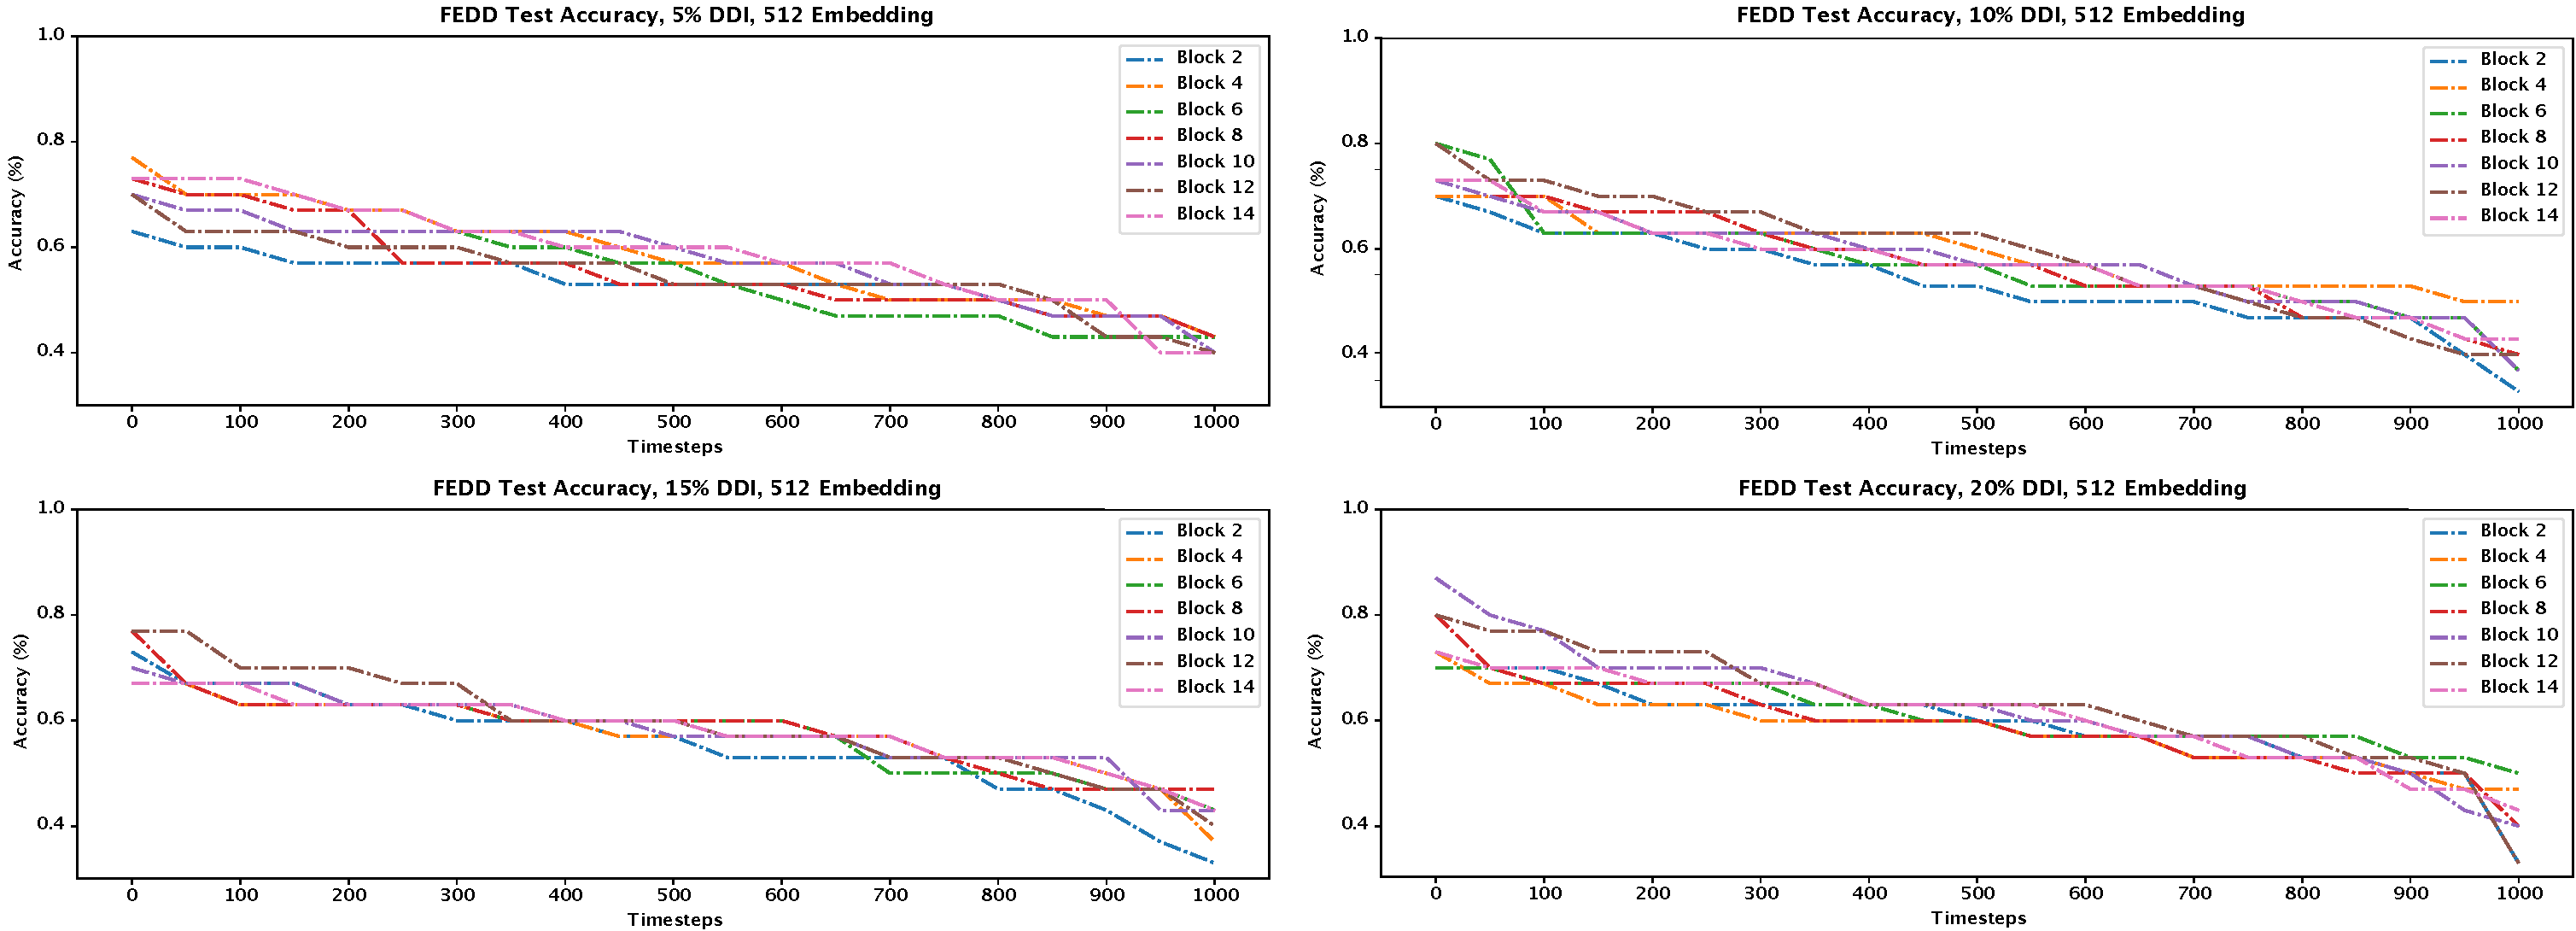
\includegraphics[width=1\textwidth]{FEDD/Fig_6.pdf}
    \caption{Classification accuracy of each DDPM UNet decoder is shown. Later steps in the reverse diffusion process produce the highest quality embeddings. When less data is available (top row), earlier blocks of the UNet decoder perform best. When more data is available (bottom row), the later, shallower blocks of the decoder perform best.}
    \label{fig:Cls_Blocks}
    %\vspace{-2mm}%Put here to reduce too much white space
\end{figure*}

We select the best-performing block-timestep combination at each data fraction for the rest of our experiments. The previous classification state-of-the-art on the DDI dataset is reported on \cite{daneshjou_2022_disparities} as the DeepDerm \cite{esteva_2017_dermatologistlevel} architecture pre-trained on HAM10000 \cite{tschandl_2018_the} and fine-tuned on DDI. We compare FEDD performance against this setup and other commonly used classifiers on each of our DDI subsets. We measure the Receiver Operating Characteristic Area Under the Curve (ROC-AUC) at the best threshold for each method, as well as F1 scores and classification accuracy. We observe that FEDD achieves a higher ROC-AUC than any other method at every data level. It also surpasses the dermatologist ensemble performance reported by \cite{daneshjou_2022_disparities}. FEDD also reports the best accuracy; however, it does not see improvement at 10\% or 15\% of DDI compared to 5\% and 20\%, as shown in Fig \ref{fig:roc_auc_acc}. When observing ROC curves for FEDD, we see that it meets or exceeds the performance of the ensemble of dermatologists, even with the smallest subset of DDI. We divide F1 scores between light and dark skin tones, finding that FEDD does not always achieve the best F1 performance with larger data subsets, namely 15\% and 20\% of DDI. This result suggests that purpose-built classification networks could have a performance advantage over diffusion embeddings applied to classification when trained on larger amounts of data. Detailed F1 results are shown in table form in the supplementary materials.

\subsubsection{Computational Performance}

The average run-time for FEDD training was about 40 minutes per MLP over 100 epochs. Memory footprint did not exceed 80GB of system memory or 40GB GPU memory after multiple runs. Inference time is approximately 1.5 images per second.

\begin{figure*}[t!]
    \centering
    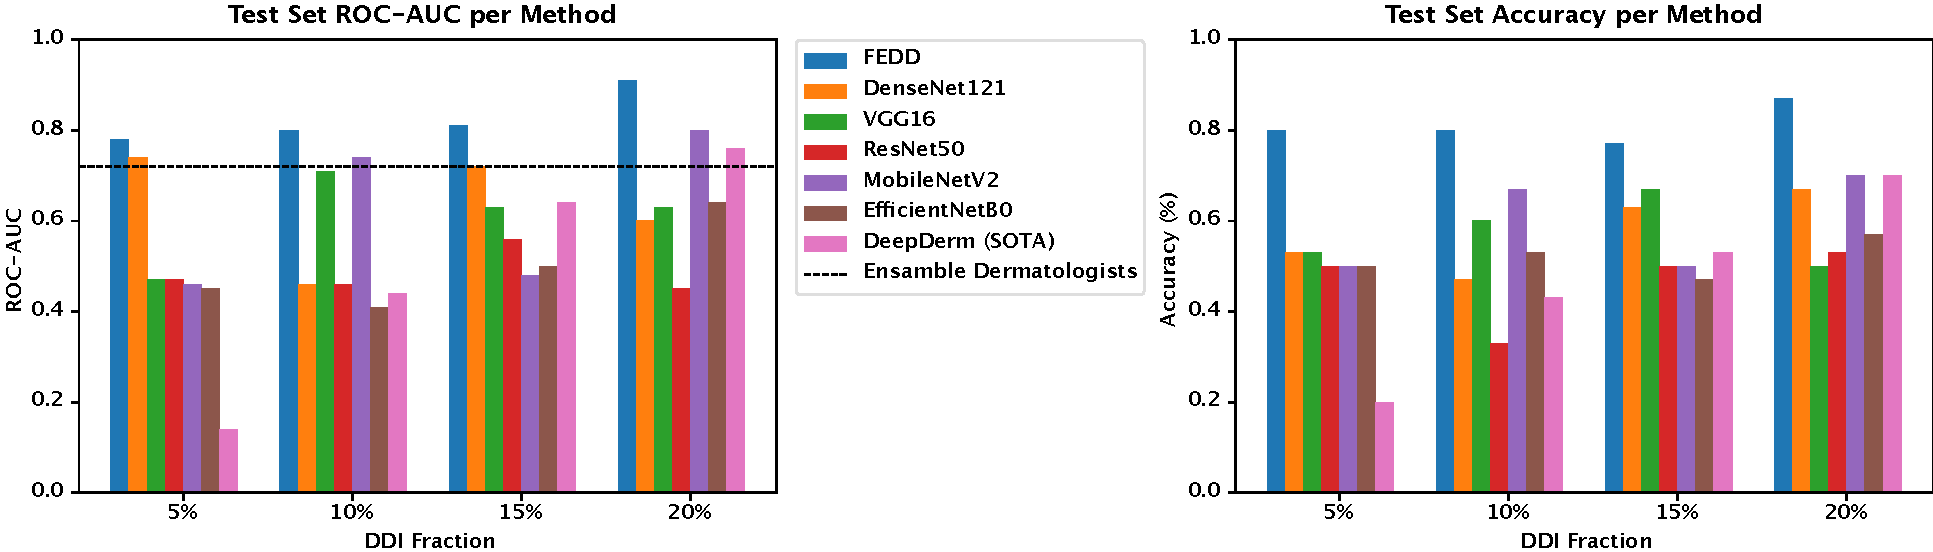
\includegraphics[width=1\textwidth]{FEDD/Fig_7.pdf}
    \caption{ROC-AUC scores (left) show FEDD outperforms other methods, including an ensemble of dermatologists. Accuracy per method is also higher (right).}
    \label{fig:roc_auc_acc}
    %\vspace{-5mm}%Put here to reduce too much white space
\end{figure*}

\begin{figure*}[t!]
    \centering
    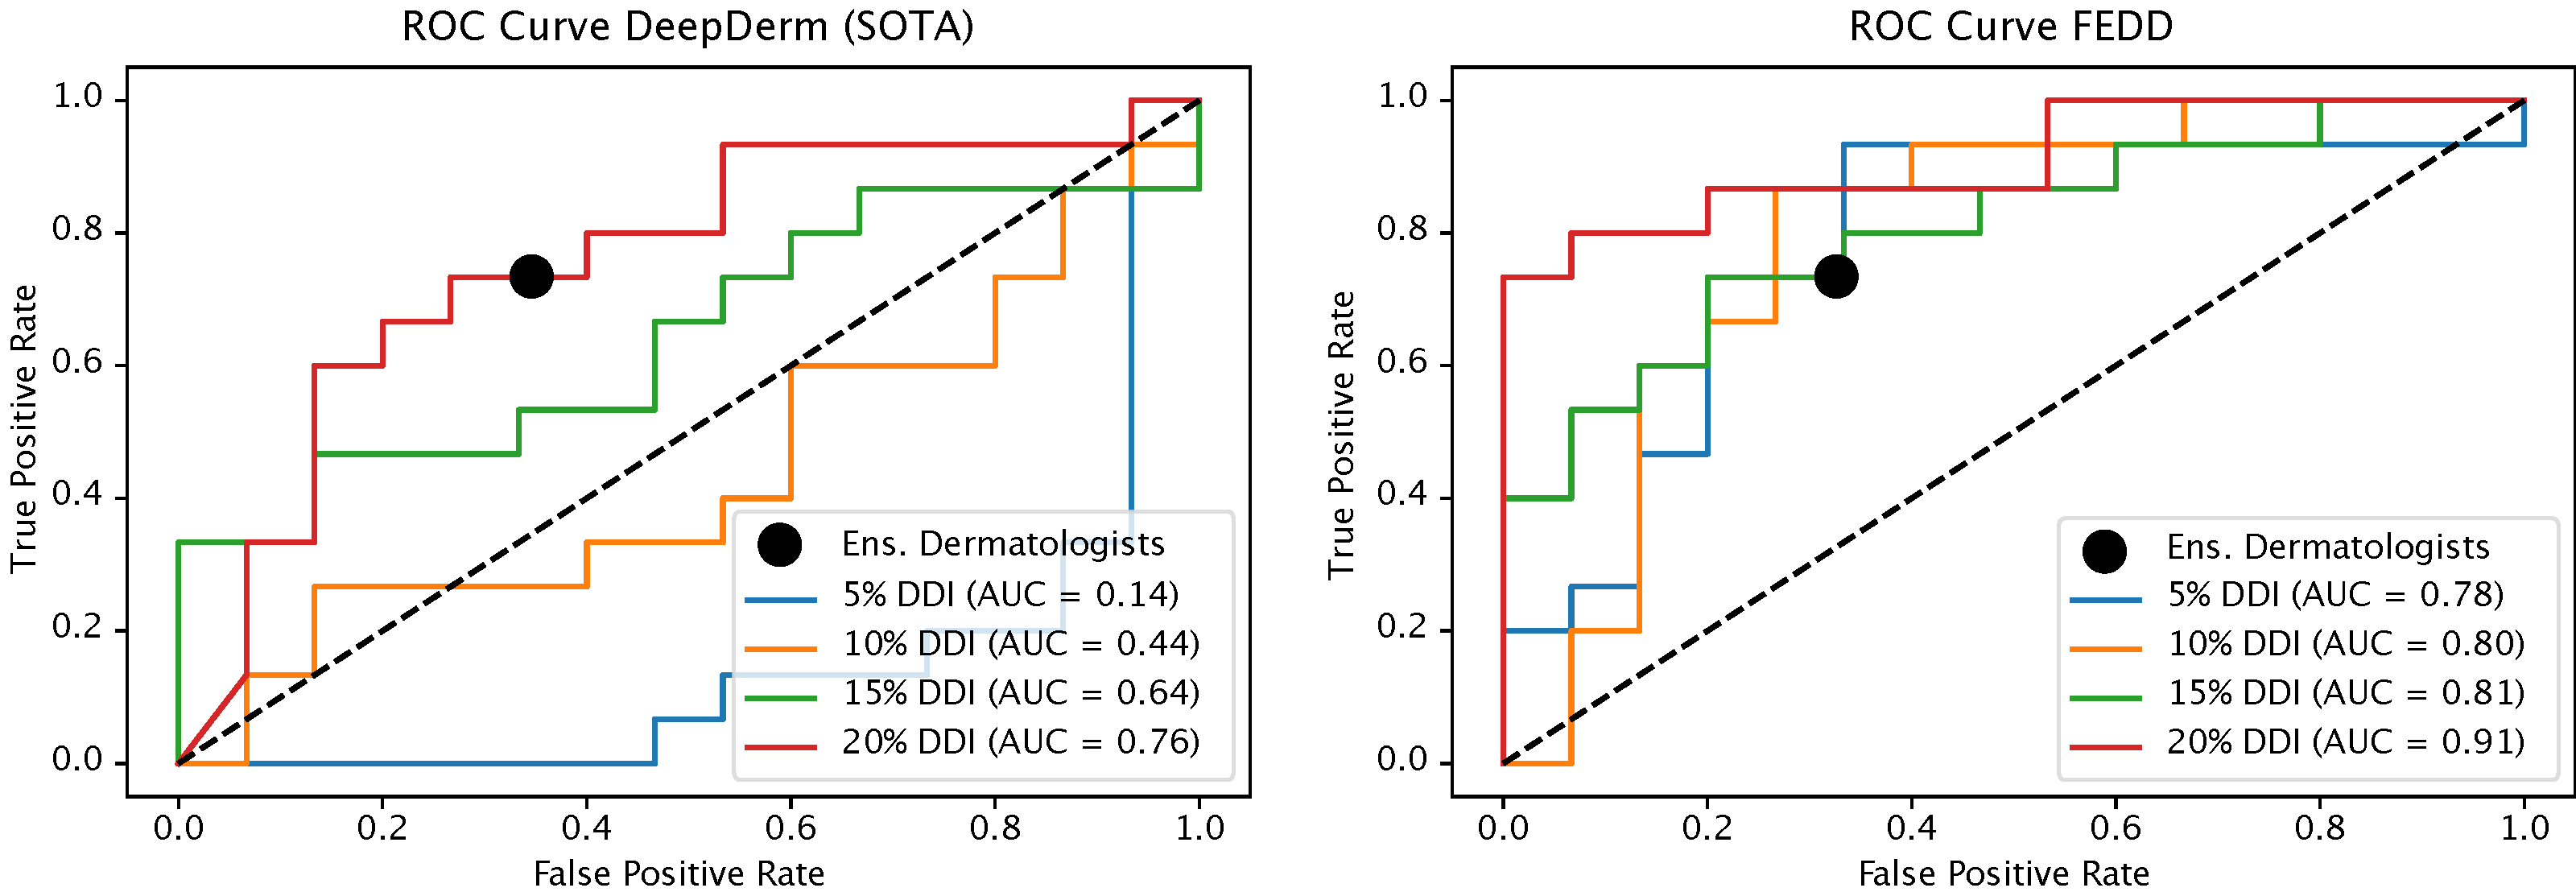
\includegraphics[width=1\textwidth]{FEDD/Fig_8.pdf}
    \caption{Test set ROC Curve for DeepDerm (left) and FEDD framework (right) at each subset of DDI data. The performance of an ensemble of dermatologists is also shown as a black circle.}
    \label{fig:roc}
    %\vspace{-5mm}%Put here to reduce too much white space
\end{figure*}

\subsubsection{K-Means Clustering}

Figure \ref{fig:KMeans} represents some examples of clustering quality for FEDD block activations and embeddings. K-Means was used with $K=3$.

\begin{figure*}[h!]
    \centering
    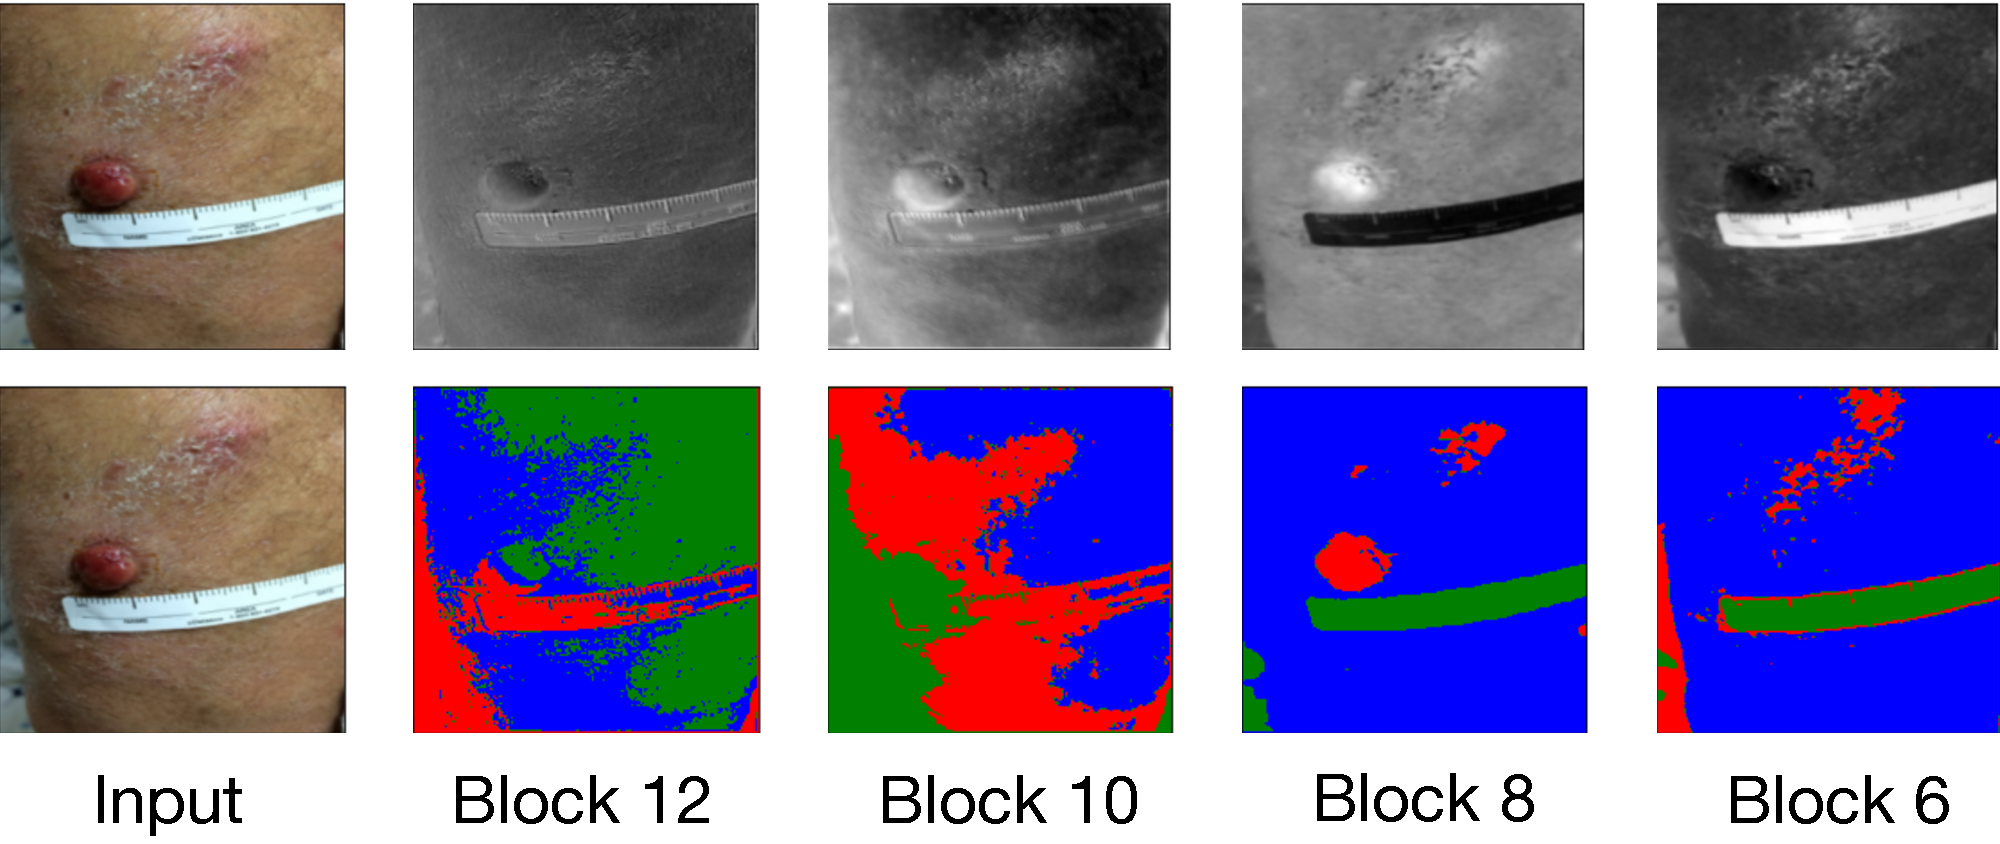
\includegraphics[width=1\textwidth]{FEDD/Fig_9.pdf}
    \caption{FEDD activation maps (top) and their clustering quality (bottom).}
    \label{fig:KMeans}
    %\vspace{-5mm}%Put here to reduce too much white space
\end{figure*}
\subsubsection{ROC Curves}

Figure \ref{fig:roc} showcases the ROC curves for previous state-of-the-art and FEDD.

\subsubsection{F1 Performance per Skin Tone}

Table \ref{tab:F1} demonstrates the F1 performance per skin tone for FEDD and all other tested architectures.

\subsubsection{Improvement Deltas}

Table \ref{tab:Deltas} demonstrates the performance advantage of FEDD versus the next best tested method.

% Table 2
\begin{table}[h!]
\centering
\caption{F1 Performance for all tested architectures split between light (left) and dark (right) skin tones.}
\resizebox{1\textwidth}{!}{
\begin{tabular}{||c|c|c|c|c|c|c|c|c||}
    \hline
    Method & 5\% DDI (Light) & 10\% DDI (Light) & 15\% DDI (Light) & 20\% DDI (Light) & 5\% DDI (Dark) & 10\% DDI (Dark) & 15\% DDI (Dark) & 20\% DDI (Dark)\\
    \hline
    DenseNet121 & 0.60 & 0.62 & 0.57 & 0.67 & \textbf{0.80} & 0.71 & 0.57 & 0.77 \\
    \hline
    VGG16 & 0.62 & 0.50 & \textbf{0.73} & 0.73 & 0.67 & 0.57 & 0.62 & 0.77 \\
    \hline
    ResNet50 & 0.00 & 0.25 & 0.29 & 0.00 & 0.33 & 0.60 & 0.50 & 0.00 \\
    \hline
    EfficientNetB0 & 0.67 & 0.00 & 0.29 & 0.62 & 0.46 & 0.00 & 0.44 & \textbf{0.91} \\
    \hline
    MobileNetV2 & 0.55 & 0.33 & 0.62 & \textbf{0.89} & 0.67 & 0.75 & 0.55 & 0.89 \\
    \hline
    DeepDerm & 0.67 & 0.00 & 0.44 & 0.60 & 0.67 & 0.50 & 0.57 & 0.75 \\
    \hline
    \textbf{FEDD} & \textbf{0.73} & \textbf{0.83} & 0.67 & \textbf{0.89} & \textbf{0.80} & \textbf{0.83} & \textbf{0.75} & 0.89 \\
    \hline
\end{tabular}
}
\label{tab:F1}
%\vspace{-10mm}%Put here to reduce too much white space after your table 
\end{table}

% Table 3
\begin{table}[h!]
\centering
\caption{Performance Improvement of FEDD compared to the next-best method on the full segmentation and classification test sets (skin-tone unbalanced).}
\begin{tabular}{||c|c|c|c|c||}
    \hline
    Metric & 5\% DDI & 10\% DDI & 15\% DDI & 20\% DDI \\
    \hline
    IoU & 0.18 & 0.13 & 0.06 & 0.07 \\
    \hline
    Accuracy & 14\% & 6\% & 5\% & 4\% \\
    \hline
\end{tabular}

\label{tab:Deltas}
%\vspace{-10mm}%Put here to reduce too much white space after your table 
\end{table}


% ============================================================
% Chapter 4 — Controllable Generation (cgDDI)
% ============================================================
\chapter{Controllable Generation, Fairness and Data Efficiency}\label{section:cgddi}

FEDD (Chapter~\ref{section:fedd}) demonstrated that frozen diffusion features plus tiny linear probes can outperform fully fine-tuned baselines and an ensemble of board-certified dermatologists on the DDI benchmark with as little as $5$--$20\%$ of the labels, while preserving performance across Fitzpatrick skin tones. But FEDD is fundamentally bounded by the data it sees: DDI contains only $656$ samples, $25$ diseases are represented by a single observation each, and the natural distribution still skews toward common diseases in light-skinned patients. No purely discriminative method can grow this distribution. This chapter inverts the question. If the bottleneck is data, generate more data --- and do so in a way that explicitly closes the demographic gaps and the rare-disease long tail. We re-use the same diffusion family that powered FEDD's discriminative features, but now in service of a controllable \emph{generator} that produces $266{,}136$ Fitzpatrick-balanced synthetic samples spanning $13$ disease conditions and three skin-tone groupings, growing DDI by more than $400\times$.

\section{cgDDI — Controllable Generation of Diverse Dermatological Imagery}\label{section:cgddi_abs}

Skin diseases impact the lives of millions of people around the world from different backgrounds and ethnicities. Therefore, accurate diagnosis in the dermatological domain requires focused work toward fairness in different skin-toned populations. However, a significant lack of expertly annotated dermatological images, especially those describing underrepresented skin tones and rare diseases, slows progress toward broadly accurate models and clear fairness metrics. In this work, we introduce \textbf{C}ontrollable \textbf{G}eneration of \textbf{D}iverse \textbf{D}ermatological \textbf{I}magery (\textbf{cgDDI}), a method capable of (1) synthesizing pixel-perfect in-distribution healthy samples, (2) lesion-mapping extremely rare lesions onto novel skin-tone combinations without training, and (3) efficient high-fidelity parametric generation with as few as $10$ training samples. Our approach is controllable via learned disease-specific prompts or skin tone descriptors, either visually or textually, allowing for the selection of key sensitive attributes. We leverage cgDDI to grow a $656$ real-image dataset by more than $400\times$. The resulting skin-tone-balanced dataset enables the development of accurate classification systems and significant improvements in essential fairness metrics. Malignancy classification experiments on the DDI benchmark show our method reaches competitive performance ($86.4\%$ accuracy) when trained exclusively on our synthetic data and state-of-the-art performance ($90.9\%$ accuracy) when fine-tuned on real data. Additionally, we achieve leading metrics for Predictive Quality Disparity, Demographic Disparity, Equality of Opportunity, as well as equitable generative image quality measurements for underrepresented skin-tones and rare diseases. We publish code, model weights, and generated datasets at \url{https://anonymous.4open.science/r/ControllableGenDDI} in support of further research in this direction.

\subsection{Background and Related Work}

Achieving fairness in medical AI requires addressing fundamental challenges in data generation for domains with severe data scarcity and demographic imbalances. Dermatological AI exemplifies these challenges: existing datasets suffer from limited expert annotations, poor representation of darker skin tones, and extreme rarity of certain conditions \cite{daneshjou_2021_lack}. While generative models offer a potential solution, current approaches require large training sets \cite{ktena-2024}, do not cover the full skin-tone spectrum \cite{wang-2024}, or ignore extremely rare diseases \cite{wang-2024}. We present a novel hybrid generation framework that addresses these limitations through complementary parametric and non-parametric approaches, achieving data-efficient synthesis while maintaining fairness across populations.

Skin diseases affect millions globally, with diagnostic accuracy among experts 4\% lower for darker-skinned patients \cite{groh-2024}, and 3 billion people lack adequate dermatological care \cite{coustasse_2019_use}. Early detection of skin cancers significantly increases survival rates \cite{balch-2009}, yet the average wait time exceeds 38 days in the United States alone \cite{tsang_2006_even}. While AI systems have shown promise in skin lesion classification \cite{winkler-2023, esteva_2017_dermatologistlevel}, a survey of 70 dermatological AI studies found less than 25\% included ethnicity and only 10\% included skin-tone descriptors \cite{daneshjou_2021_lack}. These disparities stem from technical challenges our method directly addresses:

\begin{figure}[t]
  \centering
  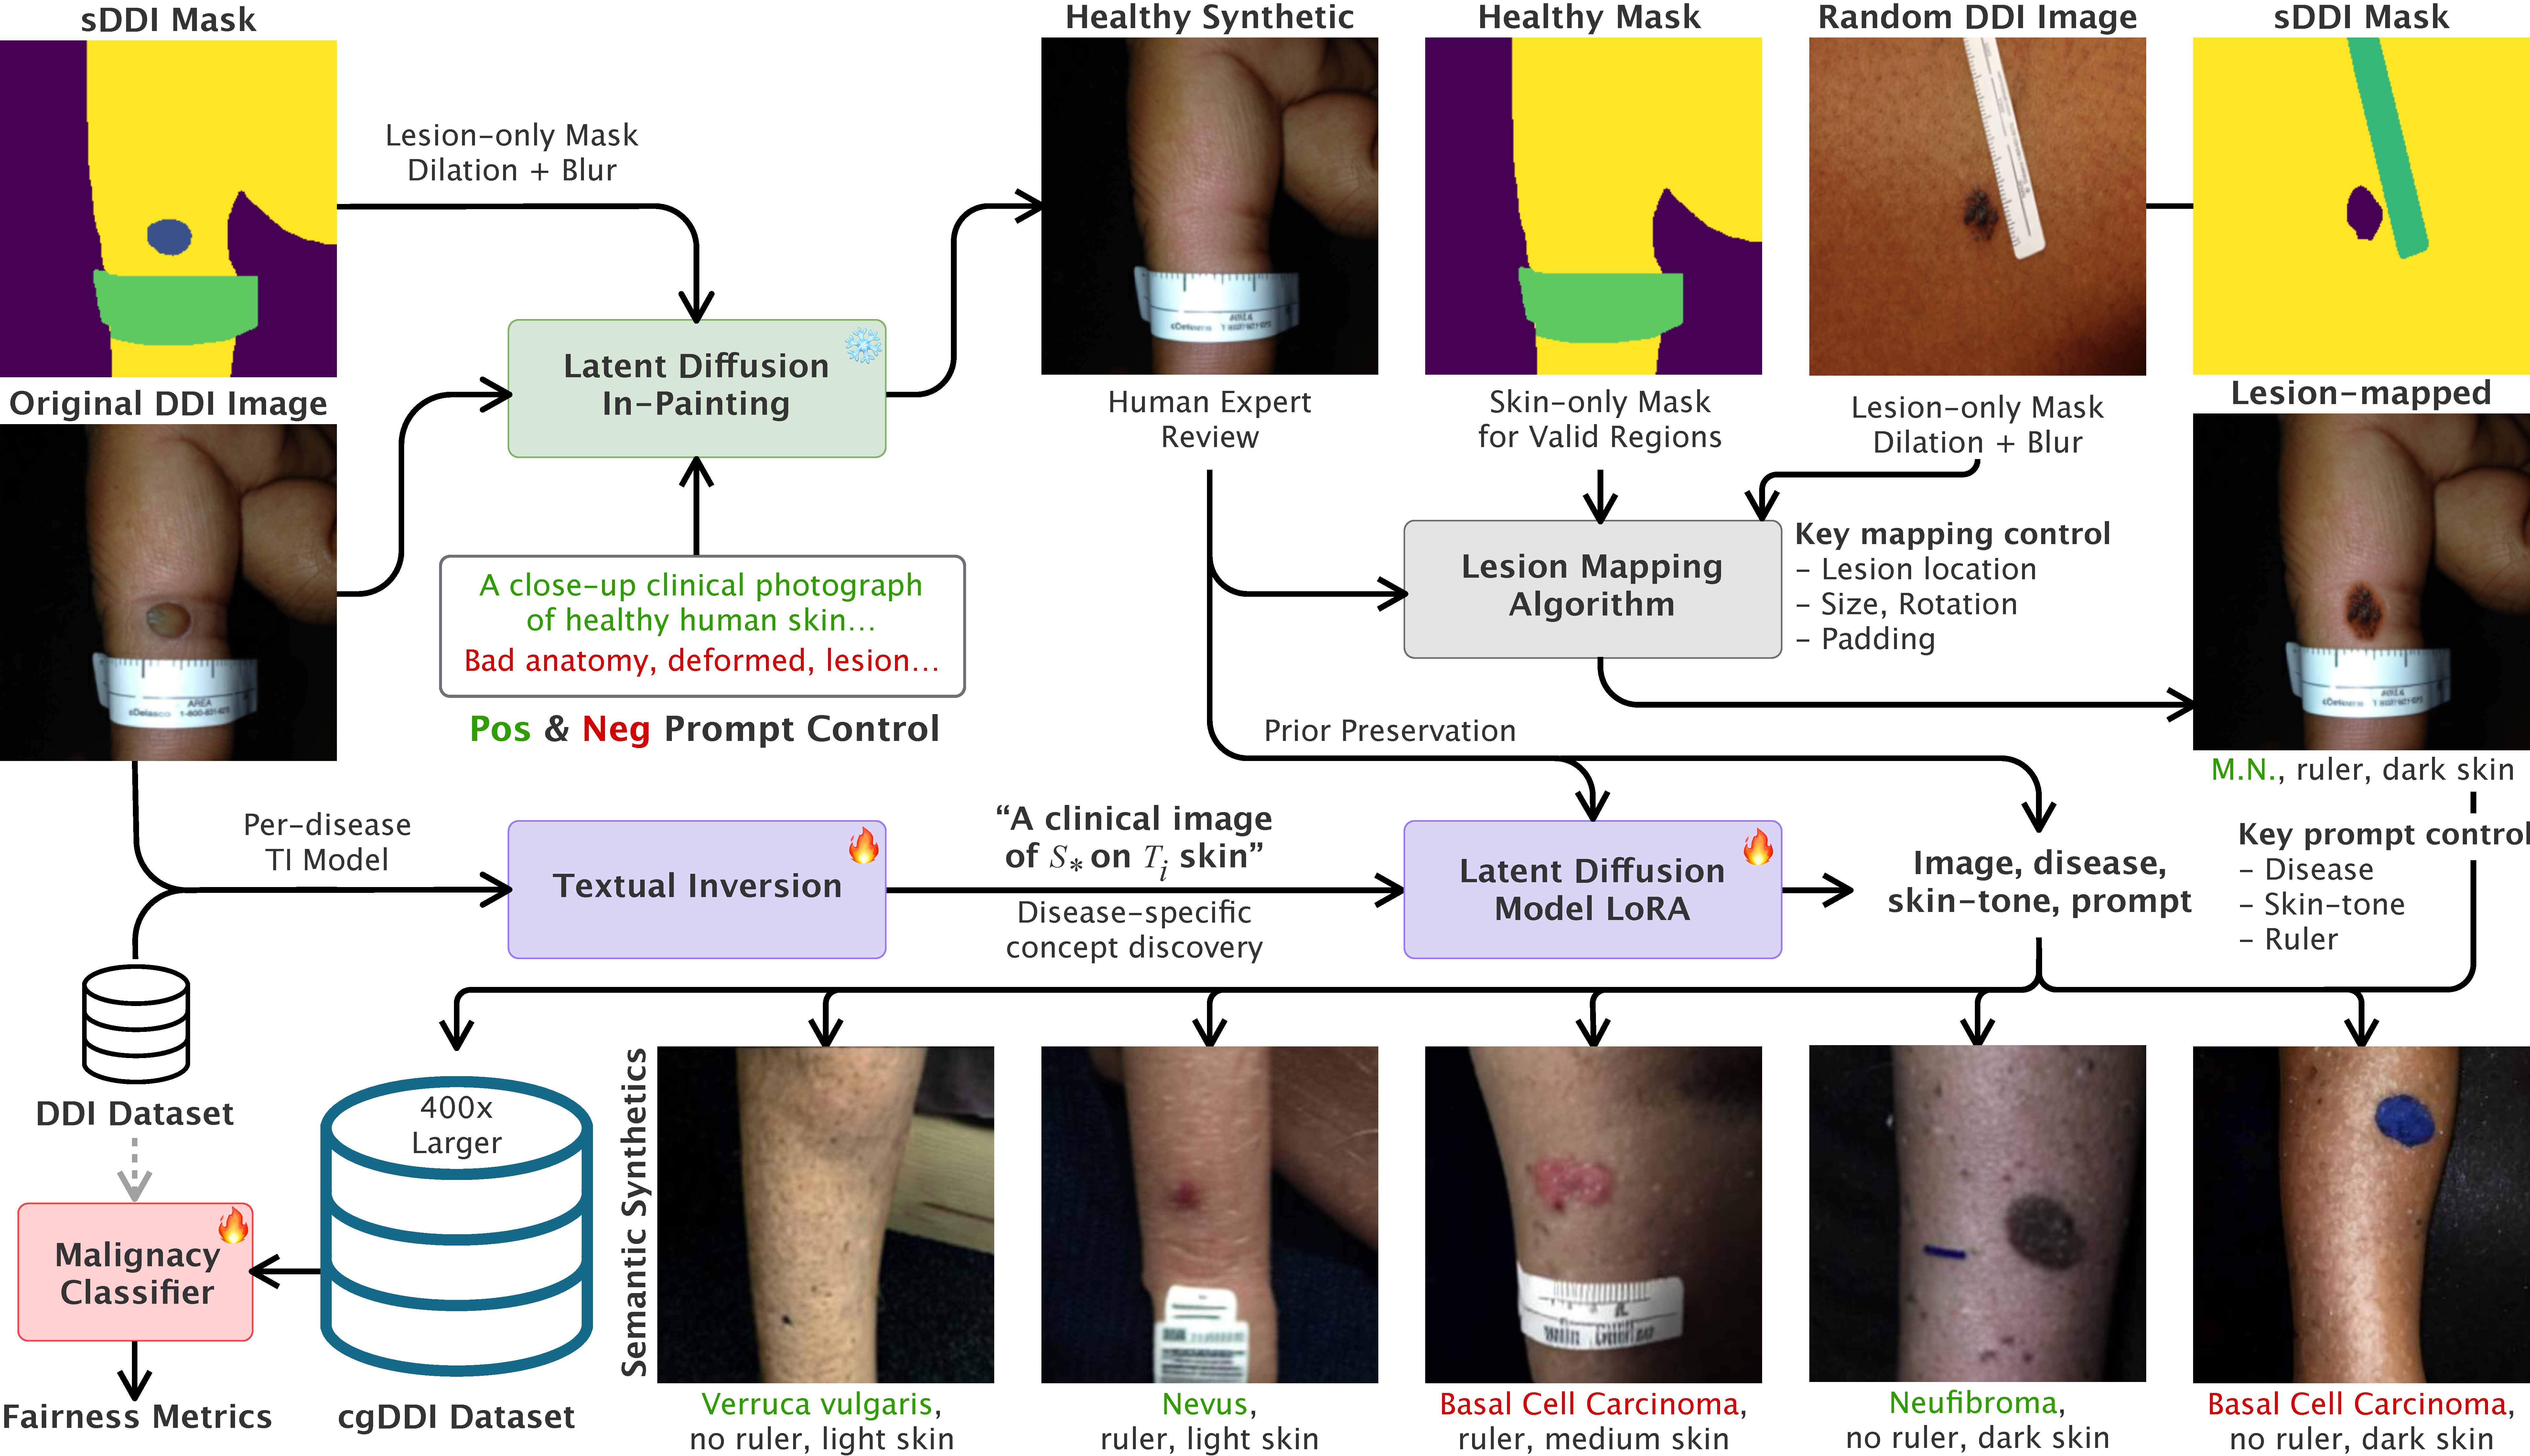
\includegraphics[width=1\linewidth]{cgDDI/cgddi_framework_colors_2.pdf}
   \caption{\textbf{cgDDI framework}. We generate dermatological synthetics in a controllable manner. First original images, masks, and prompts create \textbf{healthy synthetics}. These are used to create \textbf{lesion-mapped synthetics} from real image donors, as prior preservation, and as semantic prompts. Additionally, we learn disease-specific concepts to train a latent diffusion model from which \textbf{semantic synthetics} are sampled. Finally, cgDDI is aggregated and used to learn \textbf{fair classification} networks. Abbreviation: ``M.N." shortens Melanocytic Nevi.}
   \label{cgddi:fig:cgddi_framework}
\end{figure}

% To address this need, advances in dermatological Artificial Intelligence (AI) systems have shown effectiveness in the detection and classification of skin malignancies \cite{winkler-2023, barata-2023, grignaffini-2022}, sometimes comparable in performance to dermatologists \cite{winkler-2023, esteva_2017_dermatologistlevel, liu-2020, brinker-2019}. However, these methods are often based on data or training methods that are prone to poor performance under rare disease \cite{weng-2020, daneshjou_2022_disparities}, racial bias \cite{daneshjou_2022_disparities, owens_2020_those, chen_2021_ethical, kleinberg-2022}, or simply do not factor diversity and fairness into their work. A survey of 70 dermatological AI studies between 2015 and 2020 showed that less than 25\% included ethnicity, and only 10\% included skin-tone descriptors \cite{daneshjou_2021_lack}. We note that fair performance across populations in the dermatological domain directly necessitates work toward fairness.

% Primary obstacles impeding the development of fairness-focused research efforts include:
\begin{itemize}
    \item \textbf{Data Scarcity:} Expertly annotated medical imagery is often limited and costly to acquire due to privacy concerns, the rarity of the disease, and the availability of medical professionals, and some prior work retains these datasets for internal use only \cite{ktena-2024}.
    \item \textbf{Uneven Distribution:} The real-world distribution of various skin lesions is naturally imbalanced. This disparity is further complicated when considering skin-tone balance, especially since existing datasets are predominantly collected from light-skinned populations \cite{groh_2021_evaluating}.
    \item \textbf{Morphology and Demographics:} The morphology of the disease and general appearance can differ between individuals due to factors such as ethnicity, sex, or age \cite{adelekun_2020_skin}. Skin lesions naturally manifest in different areas of the body (e.g., face, back, leg), making it difficult to collect real-world datasets that capture the full distribution.
\end{itemize}

Simultaneously, dataset size is not the only important dimension to consider when addressing scarcity; a dataset may be large yet lack sufficient population, lesion, and morphological diversity, potentially leading to poor generalization \cite{daneshjou_2022_disparities}. These factors limit the research community's ability to develop fair and generalizable models. We present a novel hybrid generation framework that addresses fundamental challenges in synthesizing fair and diverse medical imagery under extreme data constraints. Our key methodological contributions include:

% Our cgDDI framework, outlined in Figure \ref{cgddi:fig:cgddi_framework} and discussed in Section \ref{cgddi:sec:method}, addresses these issues. In this work, we introduce the following contributions:

\begin{figure}[t]
  \centering
   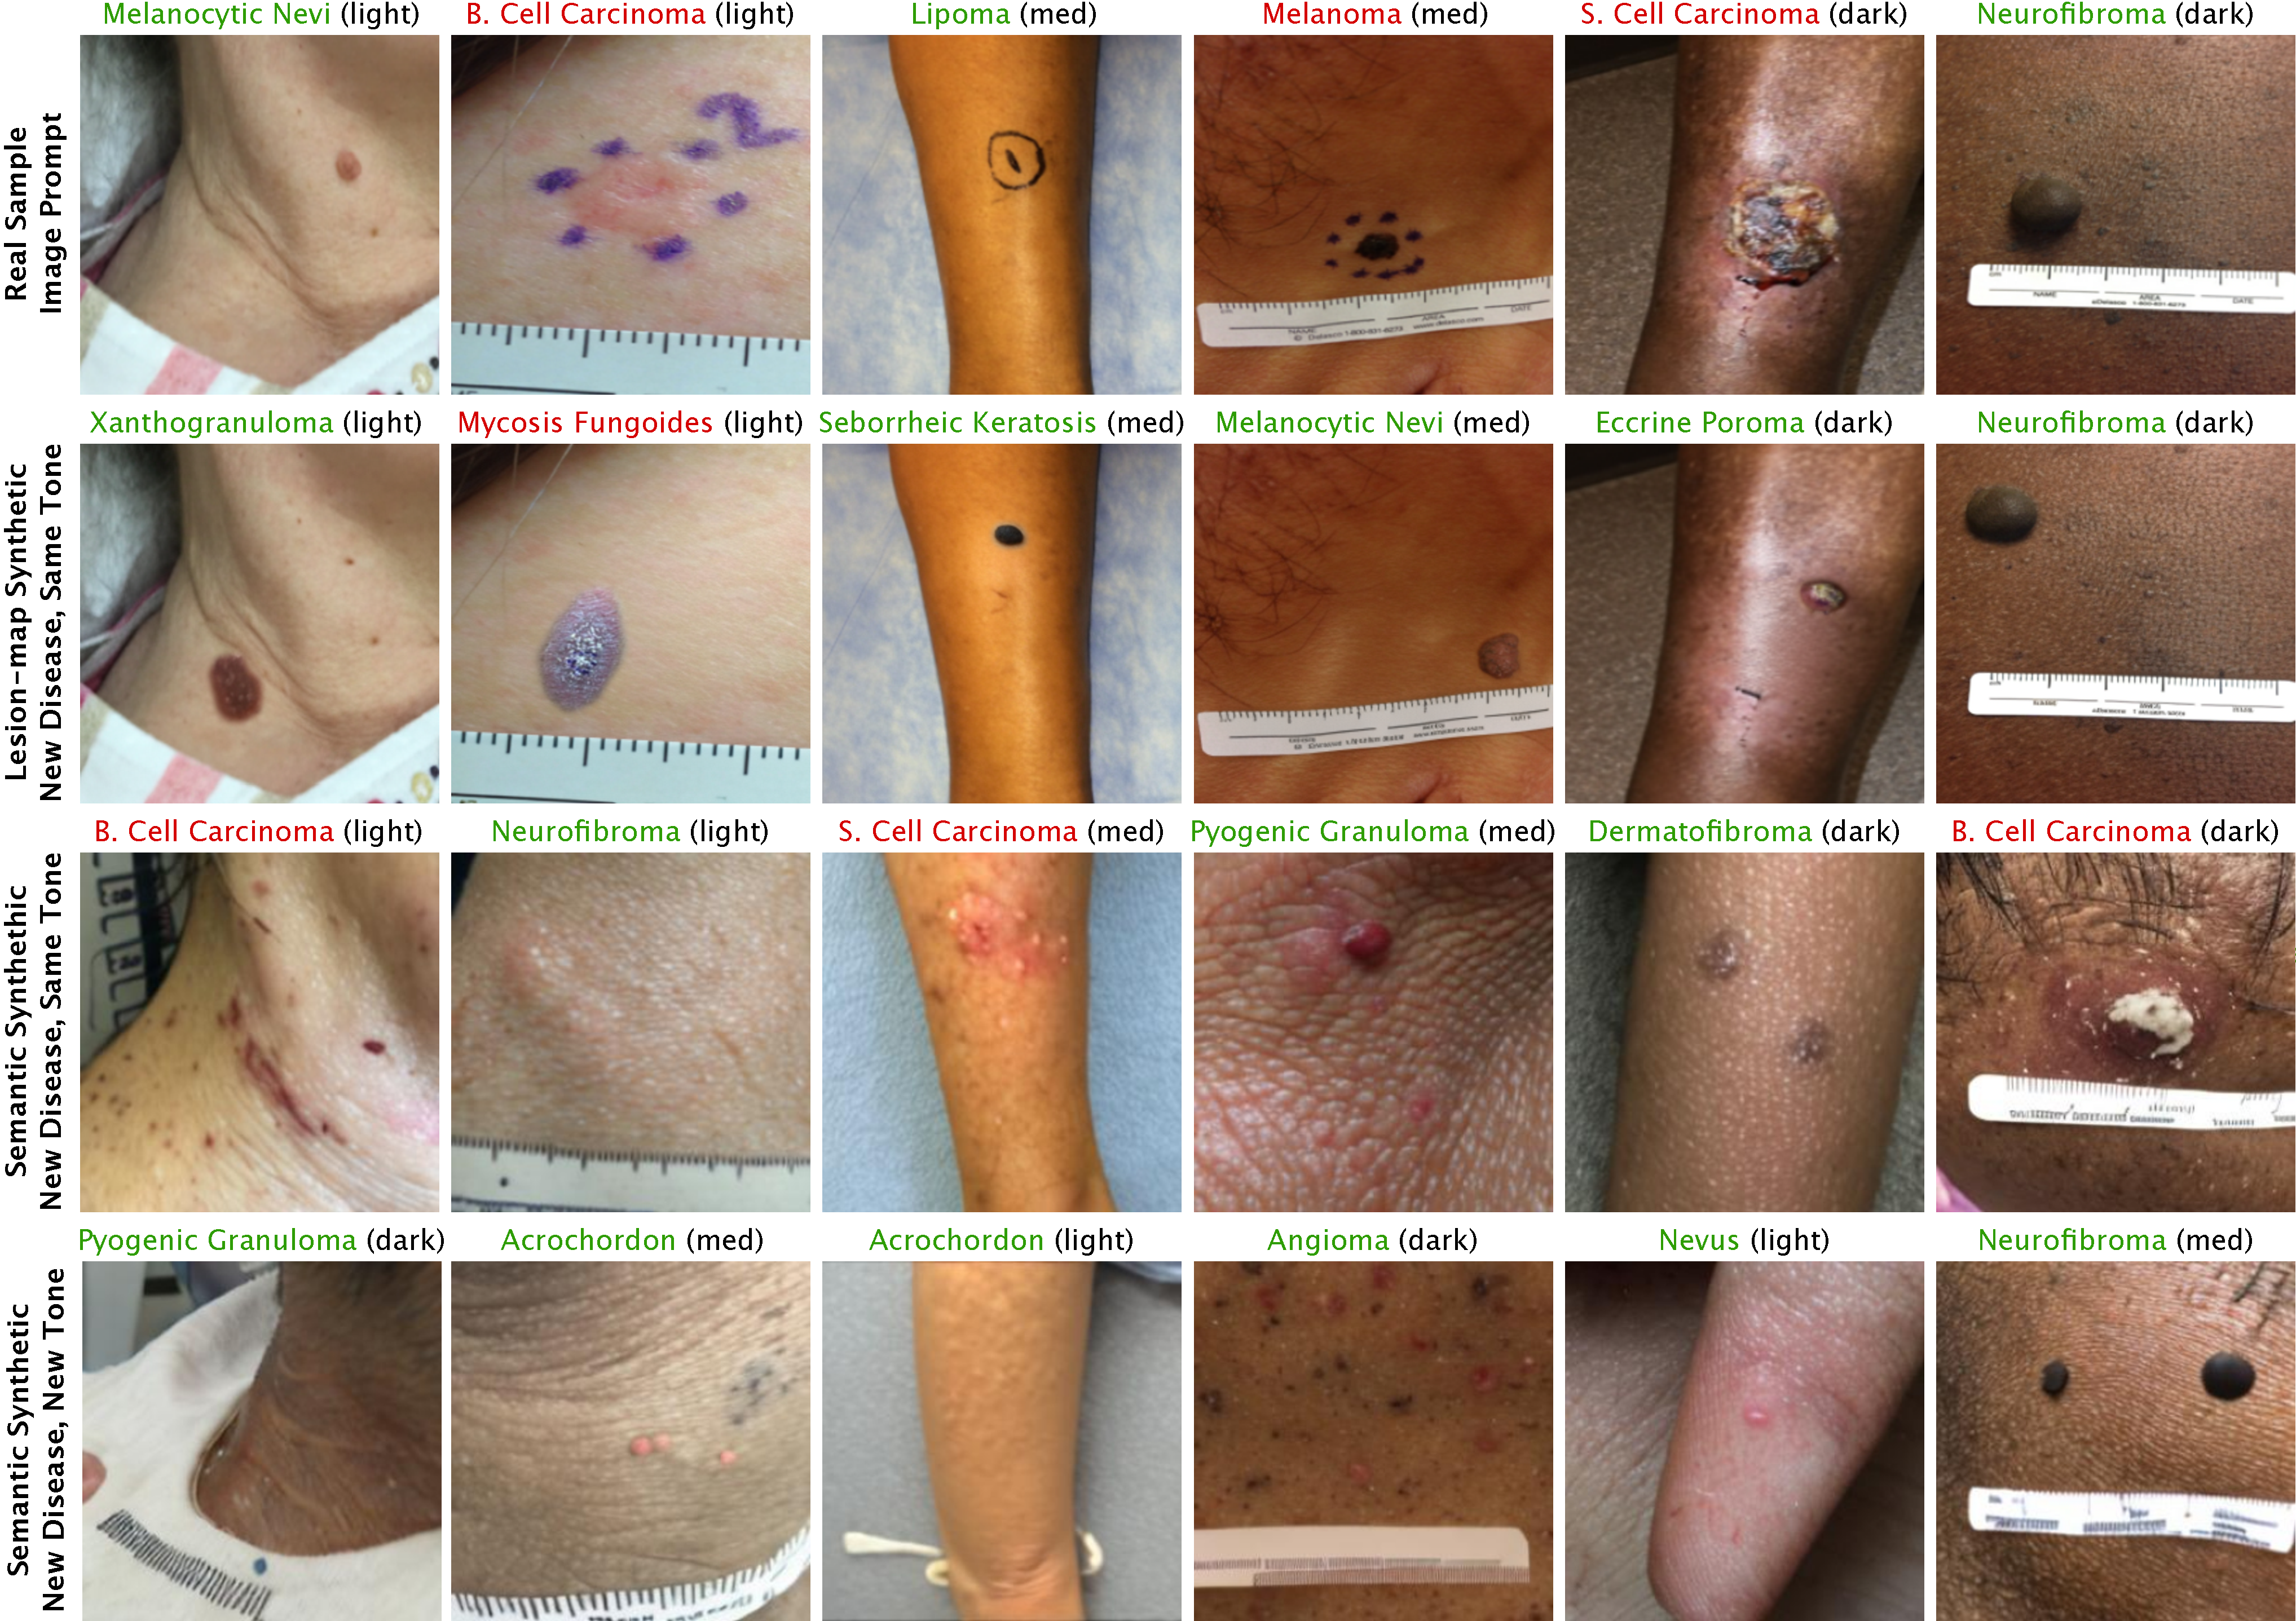
\includegraphics[width=1\linewidth]{cgDDI/cgddi_samples_final_2.pdf}
   \caption{\textbf{cgDDI Dataset}. The first row shows real samples used for prompting. The second row contains a novel lesion from a donor sample transplanted onto the prompt image. The third and fourth rows contain sampled synthetics conditioned on the prompt image, a novel target disease (\textcolor{red}{malignant} or \textcolor{green}{benign}), and a target skin tone (light, medium, or dark). Abbreviations: ``S." shortens ``Squamous", ``B." shortens ``Basal".}
   \label{cgddi:fig:cgddi_samples}
\end{figure}

\begin{itemize}
    \item \textbf{cgDDI Framework:} A method capable of dermatological image generation in a controllable manner, allowing for selection of key sensitive attributes (e.g., disease, skin-tone, etc.) or conditioned on input images for nuanced semantic control (e.g., body-part, markings, ruler, etc.). Single-sample observations are effectively augmented non-parametrically via lesion mapping, while more common cases are efficiently learned using a prior-preservation loss that leverages healthy samples for regularization. The framework is visualized in Figure \ref{cgddi:fig:cgddi_framework}.

    \item \textbf{cgDDI Dataset:} We synthesize a dataset containing three distinct data types, namely: healthy (lesion-less), lesion-mapped (from real donor images), and semantic (conditioned on learned disease and skin tone features) synthetics. Each sample is accompanied by rich metadata, including full captions, generation parameters, skin tone, condition, and malignancy. Our dataset is balanced across populations by growing a dataset of $656$ real image bases by more than $400\times$. A sample of cgDDI images is visualized in Figure \ref{cgddi:fig:cgddi_samples}.

    \item \textbf{Classification and Generative Fairness:} We measure the diagnostic quality of our data by training a malignancy classifier and evaluating various fairness metrics against real data. When training solely on our synthetic data, we achieve a competitive overall accuracy of 86.4\%. After fine-tuning on a small portion of real data, we achieve leading performance at 90.9\% overall accuracy. In both training settings, fairness metrics improve over prior work and ablate generative fairness by method and skin tone.
    
    \item \textbf{Open Datasets, Models, and Code:} We fully release all training code, models, and datasets containing 266,136 new synthetic images of three types, alongside metadata including skin tone, disease, textual captions, and other descriptors to encourage further fairness research.
\end{itemize}

\begin{table}
  \centering
  \begin{threeparttable}
    \caption{\textbf{Synthetic dermatological datasets.} Comparison across training data, fairness indicators, skin-tone coverage, controllable diseases, single-view augmentation support, dataset size, and open release. cgDDI is the only surveyed method to support single-view augmentation, achieved via its non-parametric lesion-mapping branch (Section \ref{cgddi:sec:lesion_mapping}).}
    \label{cgddi:datasets_table}
    \footnotesize
    \setlength\tabcolsep{3pt}
    \begin{tabular}{@{}lccccccc@{}}
      \toprule
      Method
        & \makecell{Training\\Data}
        & \makecell{Fairness\\Metrics}
        & \makecell{FST\\Cov.}
        & \makecell{Ctrl.\\Dis.}
        & \makecell{Single-\\view}
        & \makecell{Total\\Size}
        & \makecell{Open\\Data} \\
      \midrule
      Sagers et al. 2022~\cite{sagers-2022}
        & F17k & FST Acc. & I--VI & 3 & -- & 192 & -- \\
      Sagers et al. 2023~\cite{sagers-2023}
        & F17k, DDI & FST Acc. & I--VI & 9 & -- & 459k & \checkmark \\
      Akrout et al. 2024~\cite{akrout-2024}
        & Private & None & None & 6 & -- & 180k & -- \\
      Ktena et al. 2024~\cite{ktena-2024}
        & Private\tnote{*} & FST Gap & I--VI & 27 & -- & 50k & -- \\
      Wang et al. 2024~\cite{wang-2024}
        & F17k & FST Acc. & I--II, V--VI & 7 & -- & 7.6k & -- \\
      \midrule
      \textbf{cgDDI (ours)}
        & DDI & Multiple & I--VI & 13 & \checkmark & 266k & \checkmark \\
      \bottomrule
    \end{tabular}
    \begin{tablenotes}
      \footnotesize
      \item[]*We note \cite{ktena-2024} training data can be made available for non-commercial use upon request, payment of administrative fees, and legal compliance.
    \end{tablenotes}
  \end{threeparttable}
\end{table}

\subsubsection{Related Work}

\label{cgddi:sec:related}
\paragraph{Real Datasets} There are two main branches of dermatological datasets: dermoscopic \cite{ham, bcn}, which requires a dermatoscope magnifier, and macroscopic \cite{groh_2021_evaluating, daneshjou_2022_disparities}, which are more similar to naked eye observations. We focus our work on the latter domain, as it is more likely the type of imaging encountered in first-pass clinical practice in low-resource environments. Further, we consider datasets that contain skin tone descriptors, as these descriptors are necessary for fairness evaluation.

The most commonly cited macroscopic dataset for training and evaluating fairness in dermatological AI is Fitzpatrick17k (F17k), primarily due to its relatively large size of around 17,000 samples. However, it suffers from a skin tone imbalance, with 3.6 times as many light-skinned as dark-skinned samples, and is annotated mainly by non-experts, leading to over 30\% disease-label noise \cite{groh_2021_evaluating}. Moreover, conditions determined without biopsy or histopathological evidence might yield an unreliable ground truth \cite{daneshjou_2022_checklist}. Recent crowd-sourced datasets such as SCIN \cite{Jeong6186}, while balanced, share this limitation. The DDI dataset \cite{daneshjou_2022_disparities}, on the other hand, is fully biopsy-confirmed and verified by two board-certified dermatologists. It provides supervised Fitzpatrick-Scale (FST) \cite{fitzpatrick_1988_the} scores for skin tones across all images, categorizing them as light (I-II), medium (III-IV), or dark (V-VI), and is relatively balanced in skin tone. In addition, sDDI \cite{carrion-2023} contributes human-annotated segmentation masks for a subset of DDI images. However, the primary limitations of DDI are its small size of 656 total samples (334 of which have mask annotations in sDDI) and naturally occurring disease imbalance.

\paragraph{Generative Approaches} To address the challenges of small medical datasets, generative methods have been explored. Specifically, the success of GANs \cite{goodfellow-2020} and Diffusion Models (DMs) \cite{dhariwal_2021_diffusion} has led to their use for synthesizing photorealistic dermatology imagery \cite{wang-2024}. Controllability is a key aspect of these generation tasks, as it enables the reconstruction of sensitive attributes (e.g., disease, skin tone), an area where GANs have struggled \cite{qin-2020}. DMs, on the other hand, pre-trained for image generation conditioned on textual information, have been shown to be controllable in the dermatological domain \cite{sagers-2023}, with textual inversion \cite{gal2023an} further increasing controllability \cite{wang-2024}. Yet, these frameworks have not been shown to be effective across the full range of skin tones or under a large number of disease conditions with various frequencies. DMs have also dominated the inpainting task \cite{razzhigaev-2023}, leading to inpainting and out-painting of dermatological data \cite{sagers-2023}.

\paragraph{Synthetic Datasets} We survey recent datasets created by controllable DMs and summarize their attributes in Table \ref{cgddi:datasets_table}. Some related works do not use public training data \cite{ktena-2024}, and many do not publish their generated data \cite{wang-2024}. Two have incomplete coverage of the skin-tone range \cite{ktena-2024}, and all collect only basic fairness metrics (e.g., per-skin-tone accuracy or performance gap). We note that training on F17k \cite{groh_2021_evaluating} can yield a seemingly high visual quality due to its larger size, but disease and skin tone representations may be noisy due to unreliable ground truth, as noted earlier. Each approach has been explicitly trained to generate a distinct number of conditions, often determined by the availability of training data.

\paragraph{Classification Methods and Fairness} Dermatological classification frameworks, previously studied using CNNs \cite{han_2020_augmented}, have adopted ViT \cite{dosovitskiy-2020} or DMs-based approaches \cite{carrion-2023}, leading to increased performance. One commonality among ViTs, Large Vision Models (LVMs), and high-fidelity generative methods is that they often require large amounts of data to train effectively \cite{Moon2022FinetuningDM}, a limitation shared with the medical fairness domain. Recent studies have established the state-of-the-art in malignancy classification under DDI, in terms of both accuracy and fairness, by leveraging contrastive disentanglement \cite{du_2023_fairdisco} and patch alignment \cite{aayushman-2024} for efficient learning. Critically, these studies include a collection of informative fairness metrics. We build upon these recent works by training from scratch solely on our synthetic data, then fine-tuning on real data and computing the same metrics, as discussed in the following sections.

\subsection{Dataset}

\label{cgddi:sec:basedata}
We exclusively use DDI in our experiments because it is biopsy- and dermatologist-confirmed for both condition and skin tone, which helps avoid noise in our training process. DDI includes a range of rare, common, benign, and malignant skin lesions across all skin tones. The images were captured under varying conditions using standard RGB cameras as a representative of the first-pass examination. In total, the dataset contains 656 samples, 171 malignant and 485 benign. There are 78 unique disease labels, some of which are closely related or subgroups of each other, which we combine into a total of 65 unique disease categories, as is common in some previous work \cite{ham}. We call the dataset with 65 disease categories ``Joined DDI" and detail our grouping reasoning in the Appendix. After joining, 25 diseases are represented by a single observation, 27 by 2-10 samples, and 13 by more than 10 observations. This becomes our base dataset.

\paragraph{Data provenance and de-identification.}
This work builds exclusively on the publicly available DDI dataset \cite{daneshjou_2022_disparities}, which was collected under Stanford IRB protocol numbers 36050 and 61146. All clinical images in the original dataset were de-identified following a strict protocol that removed all Personally Identifiable Information (PII), including faces, tattoos, and unique identifiers.

No new human subjects were enrolled for this study, so no additional IRB approval was required. Our synthetic data generation further enhances privacy by creating artificial images that do not directly correspond to any real individual patient.

\subsubsection{Joined-DDI Category Grouping}
In our main manuscript, we mention consolidating 78 unique disease labels in the original DDI dataset into 65 unique disease categories in what we call ``Joined DDI." This grouping was performed based on histopathological similarity, diagnostic similarities, and standard dermatological practice.

For example, several variants of Basal Cell Carcinoma (BCC) were grouped into a single BCC category, including basal-cell-carcinoma, basal-cell-carcinoma-superficial, and basal-cell-carcinoma-nodular. Similarly, different types of melanoma (melanoma-in-situ, acral-lentiginous melanoma, nodular melanoma) were consolidated into a single melanoma category while maintaining distinctions between fundamentally different malignancies. Table~\ref{cgddi:tab:disease_groups} shows representative examples of our grouping strategy.

\begin{table}[h]
\centering
\caption{Representative examples of disease grouping from original DDI labels to Joined DDI categories}
\label{cgddi:tab:disease_groups}
\begin{tabular}{ll}
\hline
\textbf{Original DDI Labels} & \textbf{Joined DDI Category} \\
\hline
basal-cell-carcinoma & \multirow{3}{*}{basal cell carcinoma} \\
basal-cell-carcinoma-superficial & \\
basal-cell-carcinoma-nodular & \\
\hline
melanoma-in-situ & \multirow{4}{*}{melanoma} \\
melanoma-acral-lentiginous & \\
nodular-melanoma-(nm) & \\
melanoma & \\
\hline
squamous-cell-carcinoma-in-situ & \multirow{3}{*}{squamous cell carcinoma} \\
squamous-cell-carcinoma & \\
squamous-cell-carcinoma-keratoacanthoma & \\
\hline
mycosis-fungoides & \multirow{2}{*}{cutaneous T-cell lymphoma} \\
subcutaneous-t-cell-lymphoma & \\
\hline
seborrheic-keratosis-irritated & \multirow{2}{*}{seborrheic keratosis} \\
seborrheic-keratosis & \\
\hline
melanocytic-nevi & \multirow{2}{*}{nevus} \\
dysplastic-nevus & \\
\hline
verruca-vulgaris & \multirow{2}{*}{verruca vulgaris} \\
wart & \\
\hline
benign-keratosis & \multirow{2}{*}{benign keratosis} \\
inverted-follicular-keratosis & \\
\hline
atypical-spindle-cell-nevus-of-reed & \multirow{2}{*}{spindle cell nevus of Reed} \\
pigmented-spindle-cell-nevus-of-reed & \\
\hline
\end{tabular}
\end{table}

Our disease grouping strategy reduced the number of unique disease categories while preserving clinically relevant distinctions. This approach provided more samples per category for training our generative models while maintaining the dataset's diagnostic utility. The complete mapping includes 78 original DDI disease labels consolidated into 65 joined DDI categories, with the remaining categories having a one-to-one mapping between original and joined labels.

\subsubsection{Mask Annotations}
Our work builds upon the segmentation masks from sDDI \cite{carrion-2023}, which provide pixel-level annotations for four classes: skin, lesion, ruler, and marker. We applied the following post-processing steps to these masks to prepare them for our generation pipeline:

\begin{itemize}
    \item \textbf{Boundary refinement:} To ensure smooth transitions in the inpainting process, we applied a dilation operation followed by a Gaussian blur to the target mask boundaries.
    \item \textbf{Mask consolidation for healthy synthetics:} We merged lesion and marker classes into a single ``skin" as the original lesion and marker were removed and replaced with normal skin during our inpainting process.
    \item \textbf{Valid mask area:} The lesion mapping algorithm, calculates ``valid region" masks by identifying skin-only regions where lesions could be realistically placed, with or without padding. This avoids placing lesions on top of the ruler area, for example.
\end{itemize}

To ensure the sDDI \cite{carrion-2023} mask fits the image data, we also need to use the image pre-processing technique from that work. It mainly involves cropping DDI images into a square shape; more details can be found on \cite{carrion-2023}.

\begin{figure}[t]
  \centering
  \includegraphics[width=1\linewidth]{cgDDI/cgddi_bad_prompts.pdf}
   \caption{\textbf{Ablation of inpainting prompts}. We observe anatomically incorrect generation of healthy samples if we do not include terms like ``healthy, smooth normal" as guidance on the positive prompt (left). Similarly, excluding terms from the negative prompt like ``hole, transparent" (center) or ``eye" (right) yields artifacts.}
   \label{cgddi:fig:bad_prompts}
\end{figure}

\subsection{Method}

\label{cgddi:sec:method}
Our framework generates three complementary types of synthetic dermatological imagery through a sequential pipeline. Starting with DDI as the base dataset (Subsection \ref{cgddi:sec:basedata}), we develop a latent diffusion inpainting pipeline (Subsection \ref{cgddi:sec:in-painting}) to remove lesions from healthy skin samples while preserving original skin tone and image context. Although healthy skin imagery may appear readily available, to our knowledge, there is no dataset with dermatologist-verified skin tone labels collected in a setting analogous to that of diseased samples. These healthy synthetics are ideal for multiple purposes: as recipient canvases for our non-parametric lesion mapping algorithm (Subsection \ref{cgddi:sec:lesion_mapping}), which places real lesion observations onto healthy skin, and as prior preservation anchors for our parametric semantic generation approach (Subsection \ref{cgddi:sec:parametric}). We generate 309 healthy, 80,427 lesion-mapped, and 185,400 semantic synthetic images. We design a protocol to verify and triage generated data via manual review and ablation, dropping between 7\% and 22\% of synthetics depending on the method. Full details of the review criteria and final skin-tone balance are included in the Appendix. The modular design allows each method to address different data scarcity scenarios: the lack of clinical-quality baselines, extremely rare conditions, and parametric generation that scales efficiently for cases with limited but sufficient training examples.


\subsubsection{Latent Diffusion Inpainting}
\label{cgddi:sec:in-painting}

To convert DDI into healthy samples, we perform inpainting using the frozen UNet denoiser (1.22 B parameters) and MoVQGAN decoder (67 M parameters) \cite{razzhigaev-2023}, guiding the generation via positive \textit{``A close-up clinical photograph of healthy, smooth, normal human skin"} and negative \textit{``Bad anatomy, deformed, lesion, ugly, disfigured, illness, hole, transparent, eye"} prompts, which avoids artifacts common when using these methods. We ablate on different prompts and prompt structures, as well as on generation without prompts, which led to artifacts that we discuss in the Appendix. We determine the precise regions of the lesion (and the marker, if present) to inpaint using semantic segmentation masks. Finally, we apply a light Gaussian blur to the lesion and marker masks to ensure a smoother transition to healthy skin. This method is visualized in Figure \ref{cgddi:fig:cgddi_framework} color-coded as green.

\paragraph{Healthy Synthetics} For masking, we elect to use sDDI as it is human-verified and delineates the skin, ruler, marker, and lesion boundaries. However, our framework is compatible with accurate out-of-the-box segmentation algorithm output masks, as shown in Section \ref{cgddi:samv3}. Out of a possible 334 samples (number of masks), we retain 309 healthy synthetics and discard 25 samples (7\%) after human review. This review excludes any images that exhibit unnatural artifacts, as detailed in the Appendix. We observe realistic, lesion-free reconstruction of the expected normal skin under lesion- or marker-covered regions, preserving the input sample's skin tone, hair coverage, and body location. This ensures that all other original descriptors remain accurate. The results are shown in Figure \ref{cgddi:fig:healthy_samples}, with additional examples in the Appendix.

\begin{figure}[t]
  \centering
  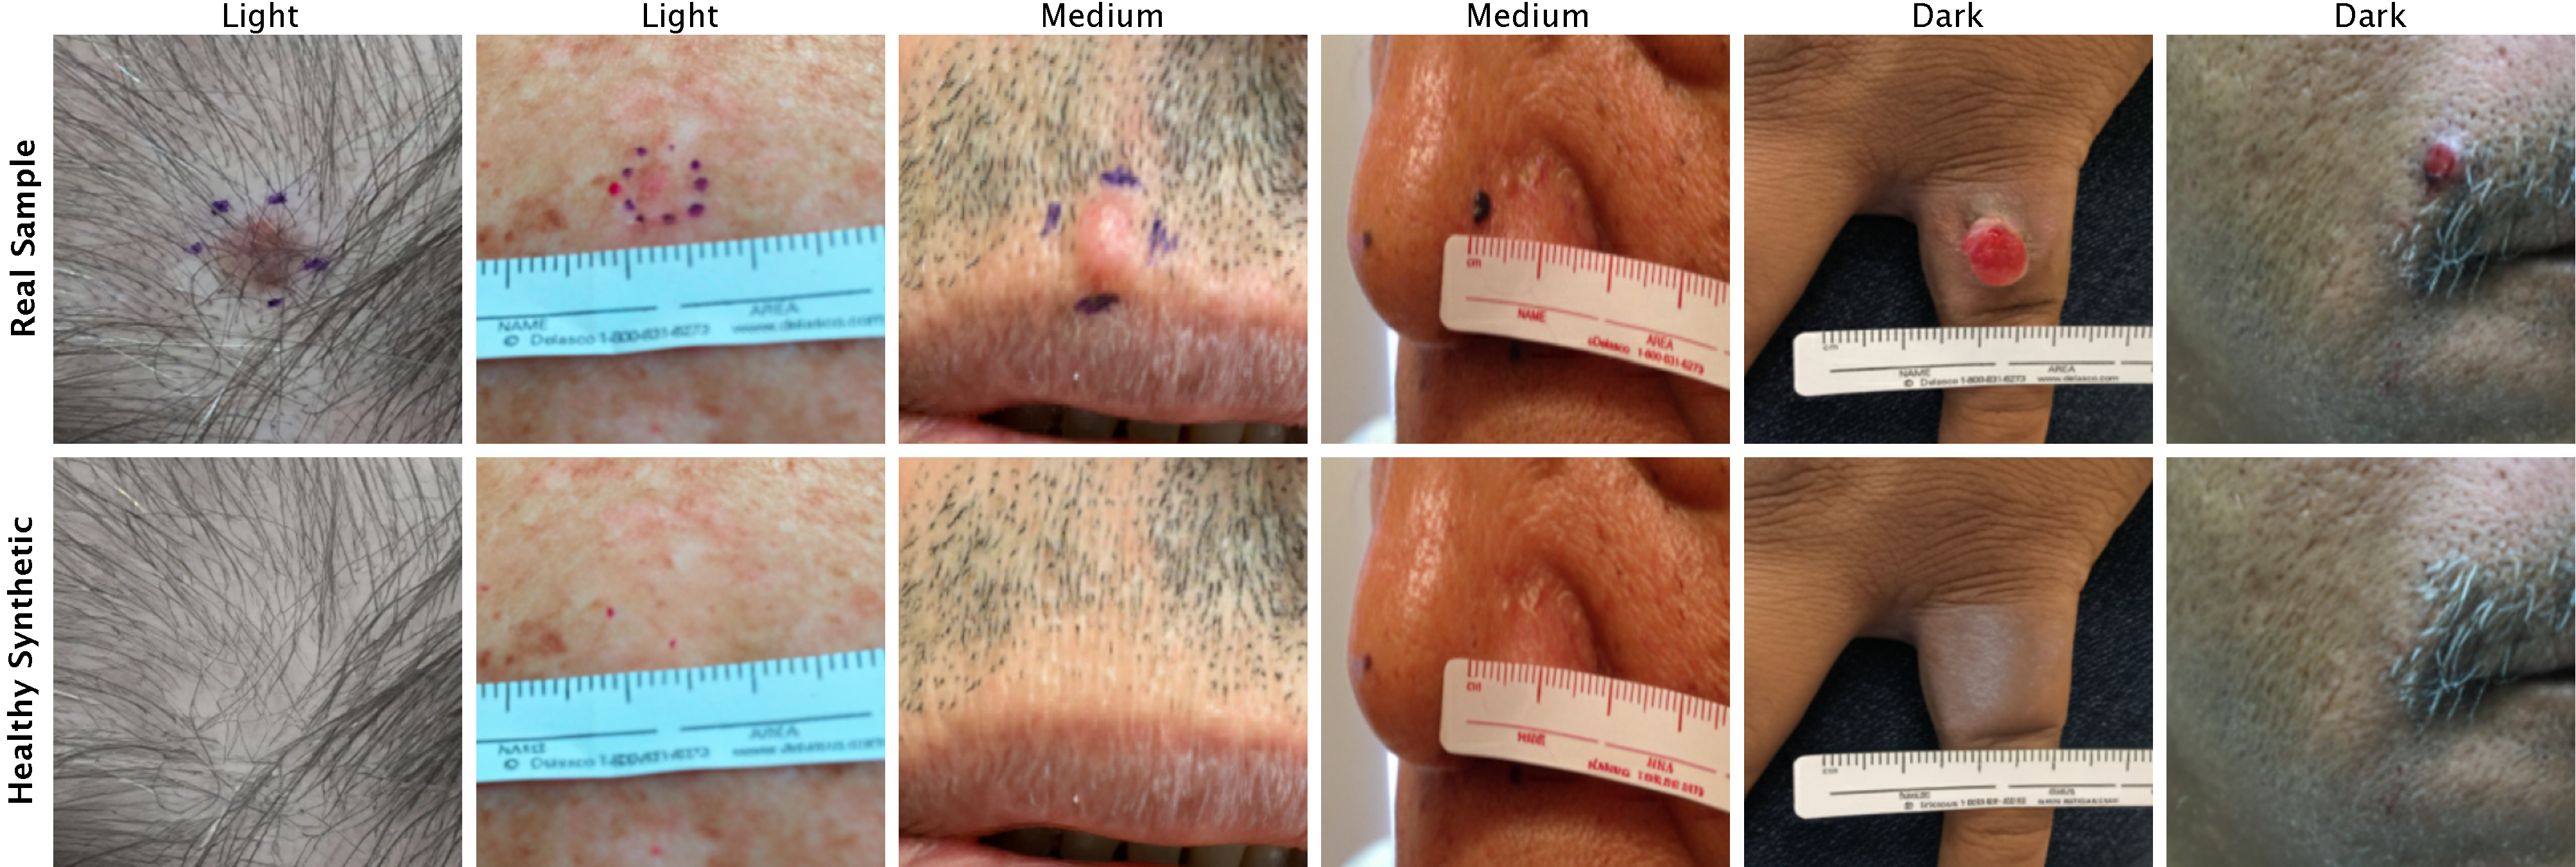
\includegraphics[width=1\linewidth]{cgDDI/cgddi_healthy_final.pdf}
   \caption{\textbf{Human-verified healthy synthetic imagery}. Our inpainting framework removes the target lesion (and any marker marks, if present). We observe lesion-less reconstruction to be robust to hair, lesion morphology, or location, ensuring skin tone descriptors remain accurate. These clinical-setting healthy samples are later leveraged toward lesion-mapped and semantic synthetic images.}
   \label{cgddi:fig:healthy_samples}
\end{figure}

\subsubsection{Lesion Mapping Algorithm}
\label{cgddi:sec:lesion_mapping}
Mapping existing lesion observations from one sample to another reduces the need to learn an accurate distribution of disease appearance and morphology, which is useful when training data is limited, as in rare diseases. However, non-parametric approaches risk placing lesions out of bounds, in differing lighting conditions, or with unnatural appearance.

Our lesion mapping algorithm alleviates these concerns by editing sDDI masks by joining previously ``lesion" or ``marker" class areas into healthy skin segments, matching our healthy synthetics. By avoiding any background or ruler sections, we explicitly determine the valid locations where a lesion can be placed. An additional padding parameter determines the minimum distance from the mask edges that a lesion edge must lie within, which helps avoid mapping lesions onto the curvature of body parts like arms, legs, or fingers. Finally, size, rotation, and position parameters can be set or left at random. This algorithm is visualized in Figure \ref{cgddi:fig:cgddi_framework}, color-coded gray.

\paragraph{Lesion-mapped Synthetics} For each healthy image, we iterate on all DDI samples with sDDI masks (donors). We dilate, then apply a light Gaussian blur to the disease mask area before mapping it onto the healthy sample. We determine a random location with padding (10 pixels from the edge). If the padding algorithm does not find enough room to place the lesion mask (as can be the case for large lesions mapped to narrow body sections), we skip it and move on to the next donor. Given 309 synthetic healthy images and 334 sDDI masks, we generate a total of 80,427 lesion-mapped samples. This total is controllable as the loop could be run multiple times with different parameters. The results are shown in the second row of Figure \ref{cgddi:fig:cgddi_samples}, with more examples in the Appendix.

\begin{figure}[t]
  \centering
  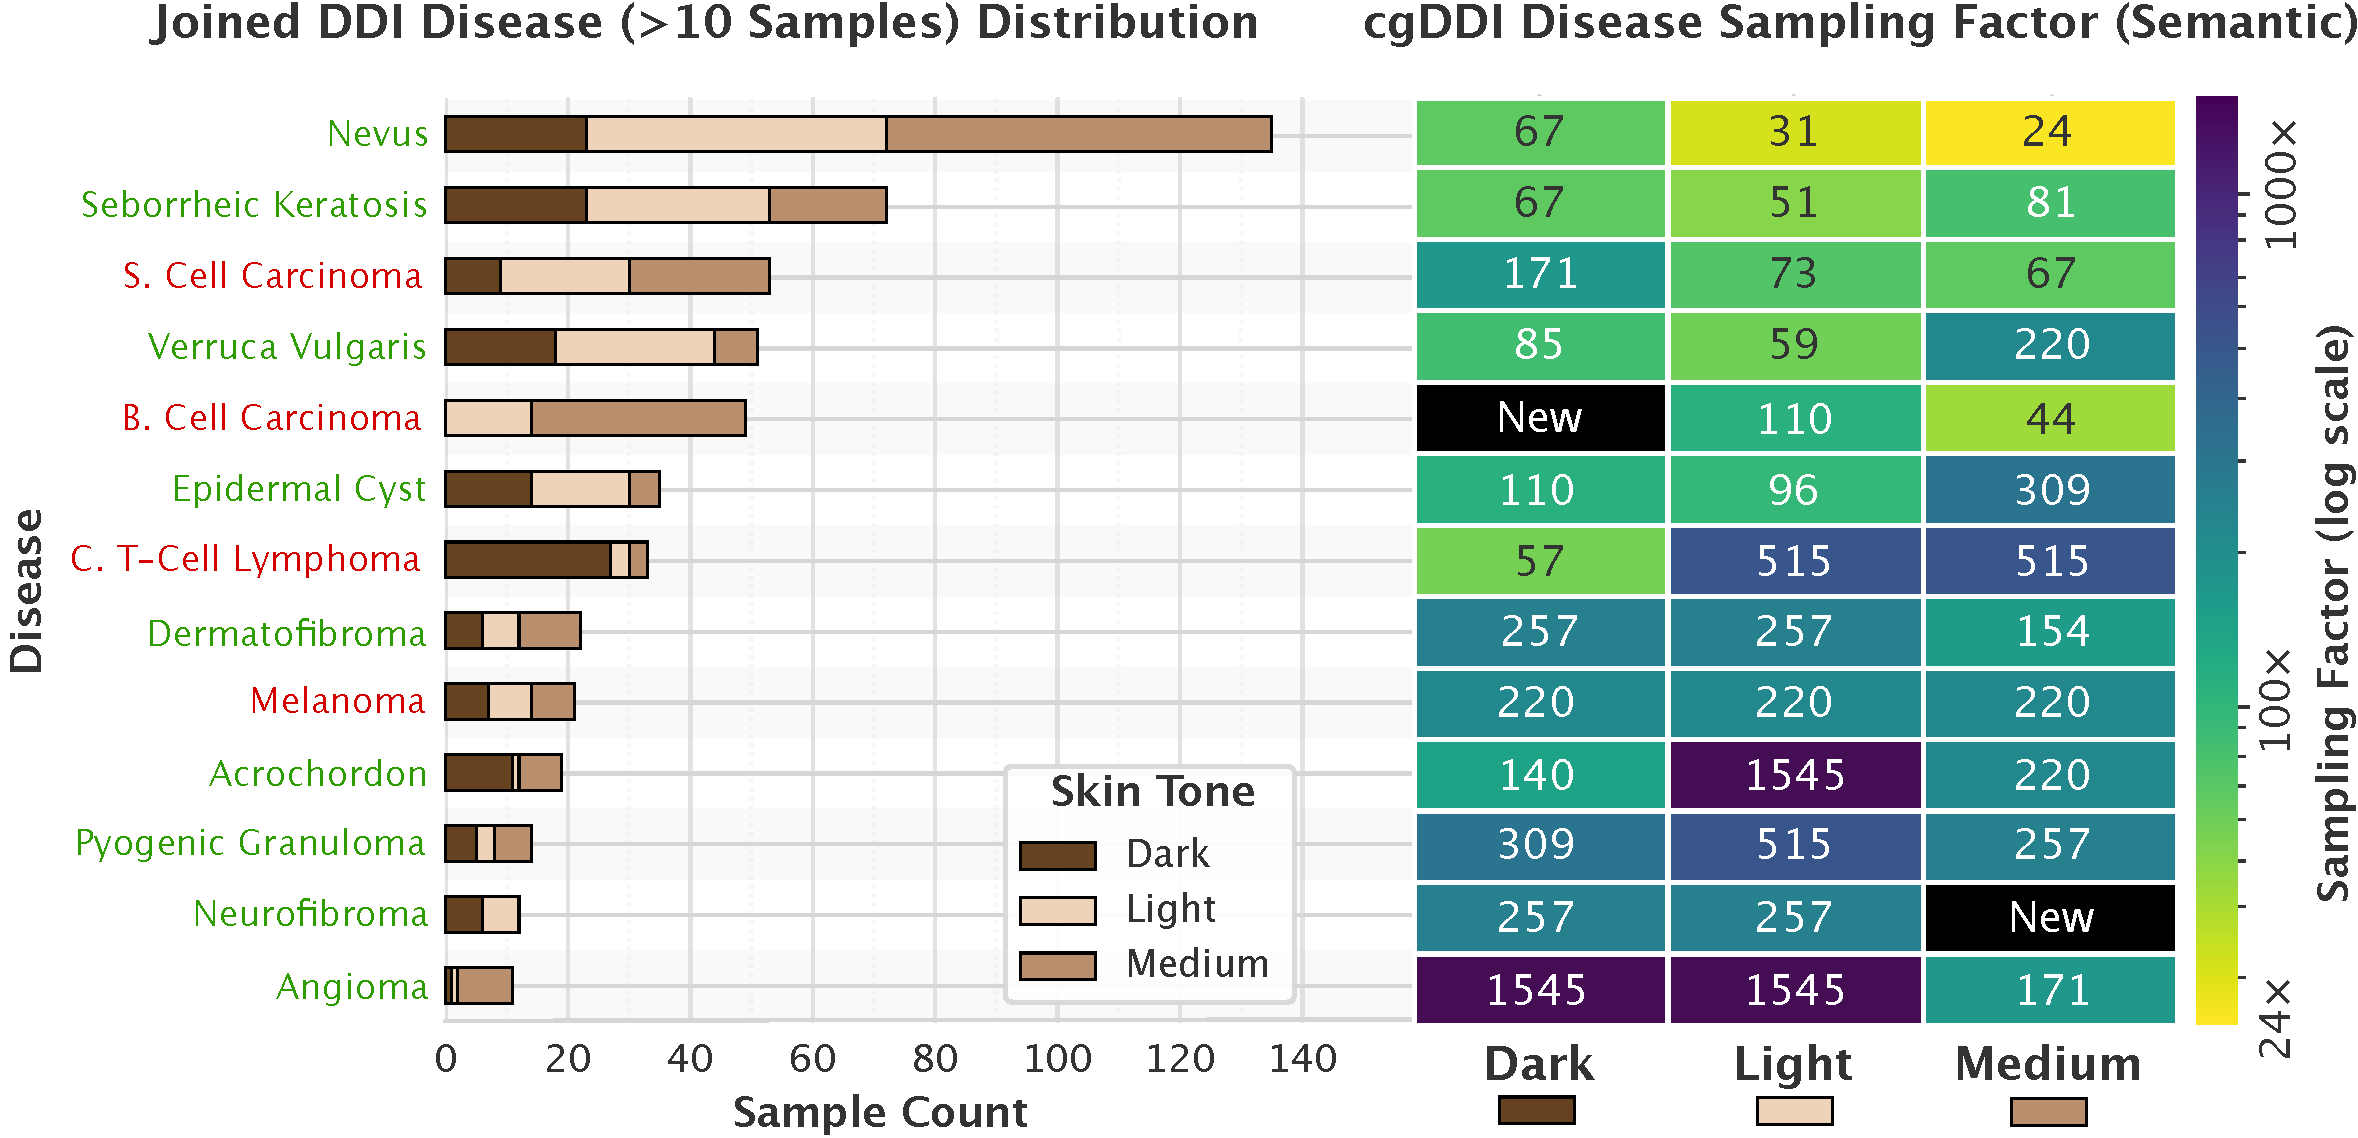
\includegraphics[width=1\linewidth]{cgDDI/distribution.pdf}
   \caption{\textbf{(Left)} Number of observations per disease and skin-tone distribution in DDI. \textbf{(Right)} Semantic sampling factor per disease and skin-tone applied to balance the distribution up to a target number of samples (4,635 total per disease). ``New" indicates that no sample of that class originally existed in DDI; cgDDI synthesized novel views up to the total balance target.}
   \label{cgddi:fig:ddi_distribution}
\end{figure}

\subsubsection{Parametric Generation}
\label{cgddi:sec:parametric}

When sufficient per-disease data is available, learned approaches for photorealistic generation and fine-grained control can be trained with high performance. As our base data is small, efficient fine-tuning algorithms and pre-trained models become our starting point. We begin by learning disease-specific tokens through textual inversion \cite{gal2023an}. These special tokens are injected into prompts used to fine-tune the latent DM backbone \cite{rombach-2022} via LoRA for parameter-efficient learning \cite{hu2022lora}. However, unlike prior work, we cover the full spectrum of skin tones, train on the smaller but more accurate Joined DDI base data, learn a greater number of unique diseases, and leverage healthy synthetics towards Prior Preservation Loss (PPL).

PPL was introduced in \cite{ruiz-2023} to address two major issues with fine-tuning DMs: forgetting semantic knowledge (drift) and reduced output diversity. Semantic drift is the decreasing ability of the network to generate class data for which a target instance belongs to (in our case, ``an image of eczema" is the class while ``an image of eczema \textit{on dark skin}" is an instance). Reduced output diversity, in our case, can limit the generation of the target from novel viewpoints, body location, skin tones, etc. Recent work has found that PPL acts as a regularizer, enabling more faithful generation than textual inversion alone \cite{zeng-2024}. We use our healthy synthetics as PPL, thereby encouraging accurate generation with a lower risk of overfitting. This process is visualized in Figure \ref{cgddi:fig:cgddi_framework}, color-coded as purple.
% Formally:

\paragraph{Semantic Synthetics} Since the number of samples needed to achieve quality results using our design is not clear a priori, we ablate the number of images needed to achieve viable quality generation. We do this by training on diseases in Joint DDI with two or more samples. We keep 10\% of the available data per disease (or at a minimum 1 sample) for testing. At generation time, let:
\begin{equation}
H=\{h_i\}_{i=1}^{309},\qquad
D=\{d_j\}_{j=1}^{40},\qquad
S=\{s_k\}_{k=1}^{3}
\end{equation}
denote our sets of healthy images, diseases, and skin tones. For each triple $(h_i, d_j, s_k)$ we draw $R=5$ independent semantic samples via:
\begin{equation}
  \begin{split}
    x_{i,j,k}^{(r)}
    &= f_{\theta,j}\Bigl(
         h_i,\;
         \underbrace{%
           \textit{“An image of }S_{*,j}\textit{ on a }s_k\textit{-toned individual”}%
         }_{\text{textual prompt}}
         \;;\;\alpha,\,\beta,\,t
      \Bigr)
  \end{split}
\end{equation}

where $f_{\theta,j}$ is the disease-specific DM, $S_{*,j}$ is the special token learned by inversion, $\alpha$ the strength factor between conditioning and pure generation, $\beta$ being the guidance scale, and $t$ the number of inference steps. Optionally, we can append “with a ruler” to the textual prompt in order to encourage a measurement overlay.

The total number of semantic synthetic images sampled is $|H|\times|D|\times|S|\times R = 185,400$, resulting in a balanced sampling of 1,545 images per skin tone and per disease. We empirically observe that around 10 samples are the minimum required to train viable generators, but we publish all imagery (along with the number of training samples) for further study. The results are shown on rows 3 and 4 of Figure  \ref{cgddi:fig:cgddi_samples}. The 13 conditions with more than 10 training samples are shown on the left side of Figure \ref{cgddi:fig:ddi_distribution} with a visualization of the sampling factor needed for balanced semantic synthetics on the right. Additional discussion on training efficiency and detailed parameter settings can be found in the Appendix.


\subsubsection{Implementation Details}

\paragraph{Latent Diffusion Inpainting: Healthy Synthetics}
Our inpainting leverages the UNet denoiser (1.22B, parameters) and MoVQGAN decoder (67M parameters) from \cite{razzhigaev-2023}. The generation process can be formalized as:

\begin{equation}
x_{\text{healthy}} = h_{\theta}(x_{\text{original}}, m, p_{\text{pos}}, p_{\text{neg}})
\end{equation}

where $x_{\text{original}}$ is the original DDI image, $m$ is the binary mask indicating areas to be inpainted (lesion or marker from sDDI \cite{carrion-2023}), $p_{\text{pos}}$ is the positive prompt guiding healthy skin generation, $p_{\text{neg}}$ is the negative prompt preventing artifacts, $h_{\theta}$ is the inpainting model with parameters $\theta$, $x_{\text{healthy}}$ is the resulting healthy synthetic image.

We experimented with various prompt templates to optimize inpainting quality. Figure \ref{cgddi:fig:bad_prompts} shows the different prompt combinations tested and their effects on the generated images.

Our optimal positive prompt was ``A close-up clinical photograph of healthy, smooth, normal human skin" and the negative prompt was ``Bad anatomy, deformed, lesion, ugly, disfigured, illness, hole, transparent, eye." This combination provided the best balance of realistic skin texture while avoiding common generation artifacts.

For mask processing, we applied a dilation with kernel size 5, followed by a Gaussian blur with $\sigma = 2.0$ to ensure smooth transitions between inpainted and original regions.

\paragraph{Non-parametric Lesion-Mapping Algorithm}
Our lesion mapping approach transfers lesions from source images to healthy synthetic images while preserving realism and anatomical context. The process can be mathematically described as:

\begin{equation}
x_{\text{mapped}} = g(x_{\text{healthy}}, x_{\text{donor}}, m_{\text{lesion}}, m_{\text{valid}}, l, p, s, r)
\end{equation}

where $x_{\text{healthy}}$ is the healthy synthetic image, $x_{\text{donor}}$ is the source image containing the lesion, $m_{\text{lesion}}$ is the lesion mask from the donor image, $m_{\text{valid}}$ is the valid region mask for the healthy image, $l$ is coordinate location of the lesion placement, $p$ is the padding parameter, $s$ is a lesion scaling multiplier, $r$ is a rotation parameter, $g$ is the mapping function, $x_{\text{mapped}}$ is the resulting lesion-mapped synthetic image.

We set the following parameters:
\begin{itemize}
    \item $l$ -- we allow the coordinate location of the mapped lesion to be determined at random, given the padding $p$ constraint.
    \item $p$ -- we set the padding parameter to 10 pixels. This means the edge of the lesion mask must be placed at least pixels from the edge of the valid skin mask.
    \item $s$ -- we set the scaling multiplier to 1.0, meaning no up or down-scaling was applied. We will investigate how to best represent the scale range of particular diseases to leverage this parameter.
    \item $r$ -- we set the rotation parameter to zero degrees, meaning no rotation was applied. We noticed that large rotations affect the natural appearance of the synthetic in relation to lighting; future work aims to automatically optimize the rotation in relation to real-world illumination.
\end{itemize}


\paragraph{Parametric Semantic Generation via Textual Inversion \& LoRA}
Our parametric generation approach learns disease-specific concepts through textual inversion and fine-tunes the latent diffusion model via LoRA. The process is formalized as:

\begin{align}
S_{*,j} &= \text{TextualInversion}(D_j, \phi) \\
\theta_j &= \text{LoRAFineTuning}(\theta, D_j, S_{*,j}, x_{\text{healthy}}) \\
x_{i,j,k}^{(r)} &= f_{\theta_j}(h_i, \text{"An image of $S_{*,j}$ on a $s_k$-toned individual"}; \alpha, \beta, t)
\end{align}

where $D_j$ is the set of training images for disease $j$, $\phi$ are the parameters of the text encoder, $S_{*,j}$ is the learned special token for disease. For fine-tuning $j$, $\theta$ are the base model parameters, $\theta_j$ are the LoRA-adapted parameters for disease $j$. Sampling is finally done with $h_i$ as the $i$-th healthy synthetic image, $s_k$ is the $k$-th skin tone, $\alpha$ is the strength factor, $\beta$ is the guidance scale, $t$ is the number of inference steps, $x_{i,j,k}^{(r)}$ is the $r$-th semantic synthetic sample for healthy image $i$, disease $j$, and skin tone $k$.

We set the following parameters:
\begin{itemize}
    \item $\alpha$ -- we set the strength factor to 0.725; we observe that setting $\alpha$ much lower than 7.0 struggles to guide generation towards the prompted skin tone.
    \item $\beta$ -- we set the guidance scale to 8.75.
    \item $t$ we set the number of inference steps to 100.
\end{itemize}

\begin{figure}[t]
  \centering
  \includegraphics[width=1\linewidth]{cgDDI/cgddi_training_samples.png}
   \caption{\textbf{Data Efficiency Ablation}. We randomly sample three subsets of semantic synthetics, equally distributed across target skin tones. We observe increasing quality with increasing training data, noting better human anatomy, increasingly realistic rulers, lesion quality, and instruction following.}
   \label{cgddi:fig:sample_ablation}
\end{figure}

\paragraph{Training Hyperparameters}

We discuss our training hyperparameters here; they can also be found in the code repository. As the inpainting pipeline is frozen, it does not necessitate training hyperparameters. The lesion mapping algorithm is non-parametric, so it does not require hyperparameters.

\paragraph{Textual Inversion}
For textual inversion, we set batch size to 4, maximum training steps to 500, learning rate to $5.0e^{-4}$, initializer token set to ``skin" and training is done at ``fp16" precision. We do not use learning rate warm-up; we use a constant learning rate schedule.

\paragraph{LoRA Fine-Tuning}
For LoRA fine-tuning, we set batch size to 16, sampling batch size is also set to 16, we set one step of gradient accumulation, maximum training steps to 750, learning rate to $5.0e^{-6}$, we point to our healthy images as class images, and training is done at ``fp16" precision. We do not leverage learning rate warm-up, and we set a constant learning rate schedule.

\paragraph{Ablations on Data Efficiency}
To determine the minimum number of real samples needed for effective generation, we conducted ablation studies on the relationship between training sample size and generation quality by visually inspecting random subsets of the generated samples. Figure~\ref{cgddi:fig:sample_ablation} shows generation results with varying numbers of training samples.

Our findings indicate that generation quality improves significantly up to approximately 10 samples, after which gains become more incremental. We specifically note improvements in human anatomy, valid clinical rulers, lesion morphology (with the isolation of the target disease rather than generating multiple lesions), and instruction following. Thus, we determine our approach is effective with as few as 10 real training samples per disease class.

\subsubsection{Review Protocol and Discard Criteria}

\begin{figure}[t]
  \centering
  \includegraphics[width=1\linewidth]{cgDDI/cgddi_healthy_2.pdf}
   \caption{\textbf{Accepted Healthy Synthetics}. Further visualization of samples that passed our review protocol.}
   \label{cgddi:fig:healhty_2}
\end{figure}

To evaluate the quality of our synthetic images, we establish a review protocol. The review was conducted by the paper authors, who have previous experience in dermatological AI research.

\paragraph{Healthy Synthetics}
\label{cgddi:ref:healthy_discard}
As there is a maximum possible 334 synthetics for this type, it was viable to manually review the full set of images.

The discard criteria are as follows:
\begin{enumerate}
    \item Original lesion remains present.
    \item Unrealistic skin texture.
    \item Incorrect skin tone.
    \item Generative artifacts (unexpected holes, eyes, lighting, etc).
\end{enumerate}

After review, we retain 309 healthy synthetics, discarding 25 (7\%) of the possible samples. Some illustrations of images that would trigger a discard appear on Figure \ref{cgddi:fig:bad_prompts} with accepted samples shown on Figure \ref{cgddi:fig:healhty_2}.

\begin{figure}[t]
  \centering
  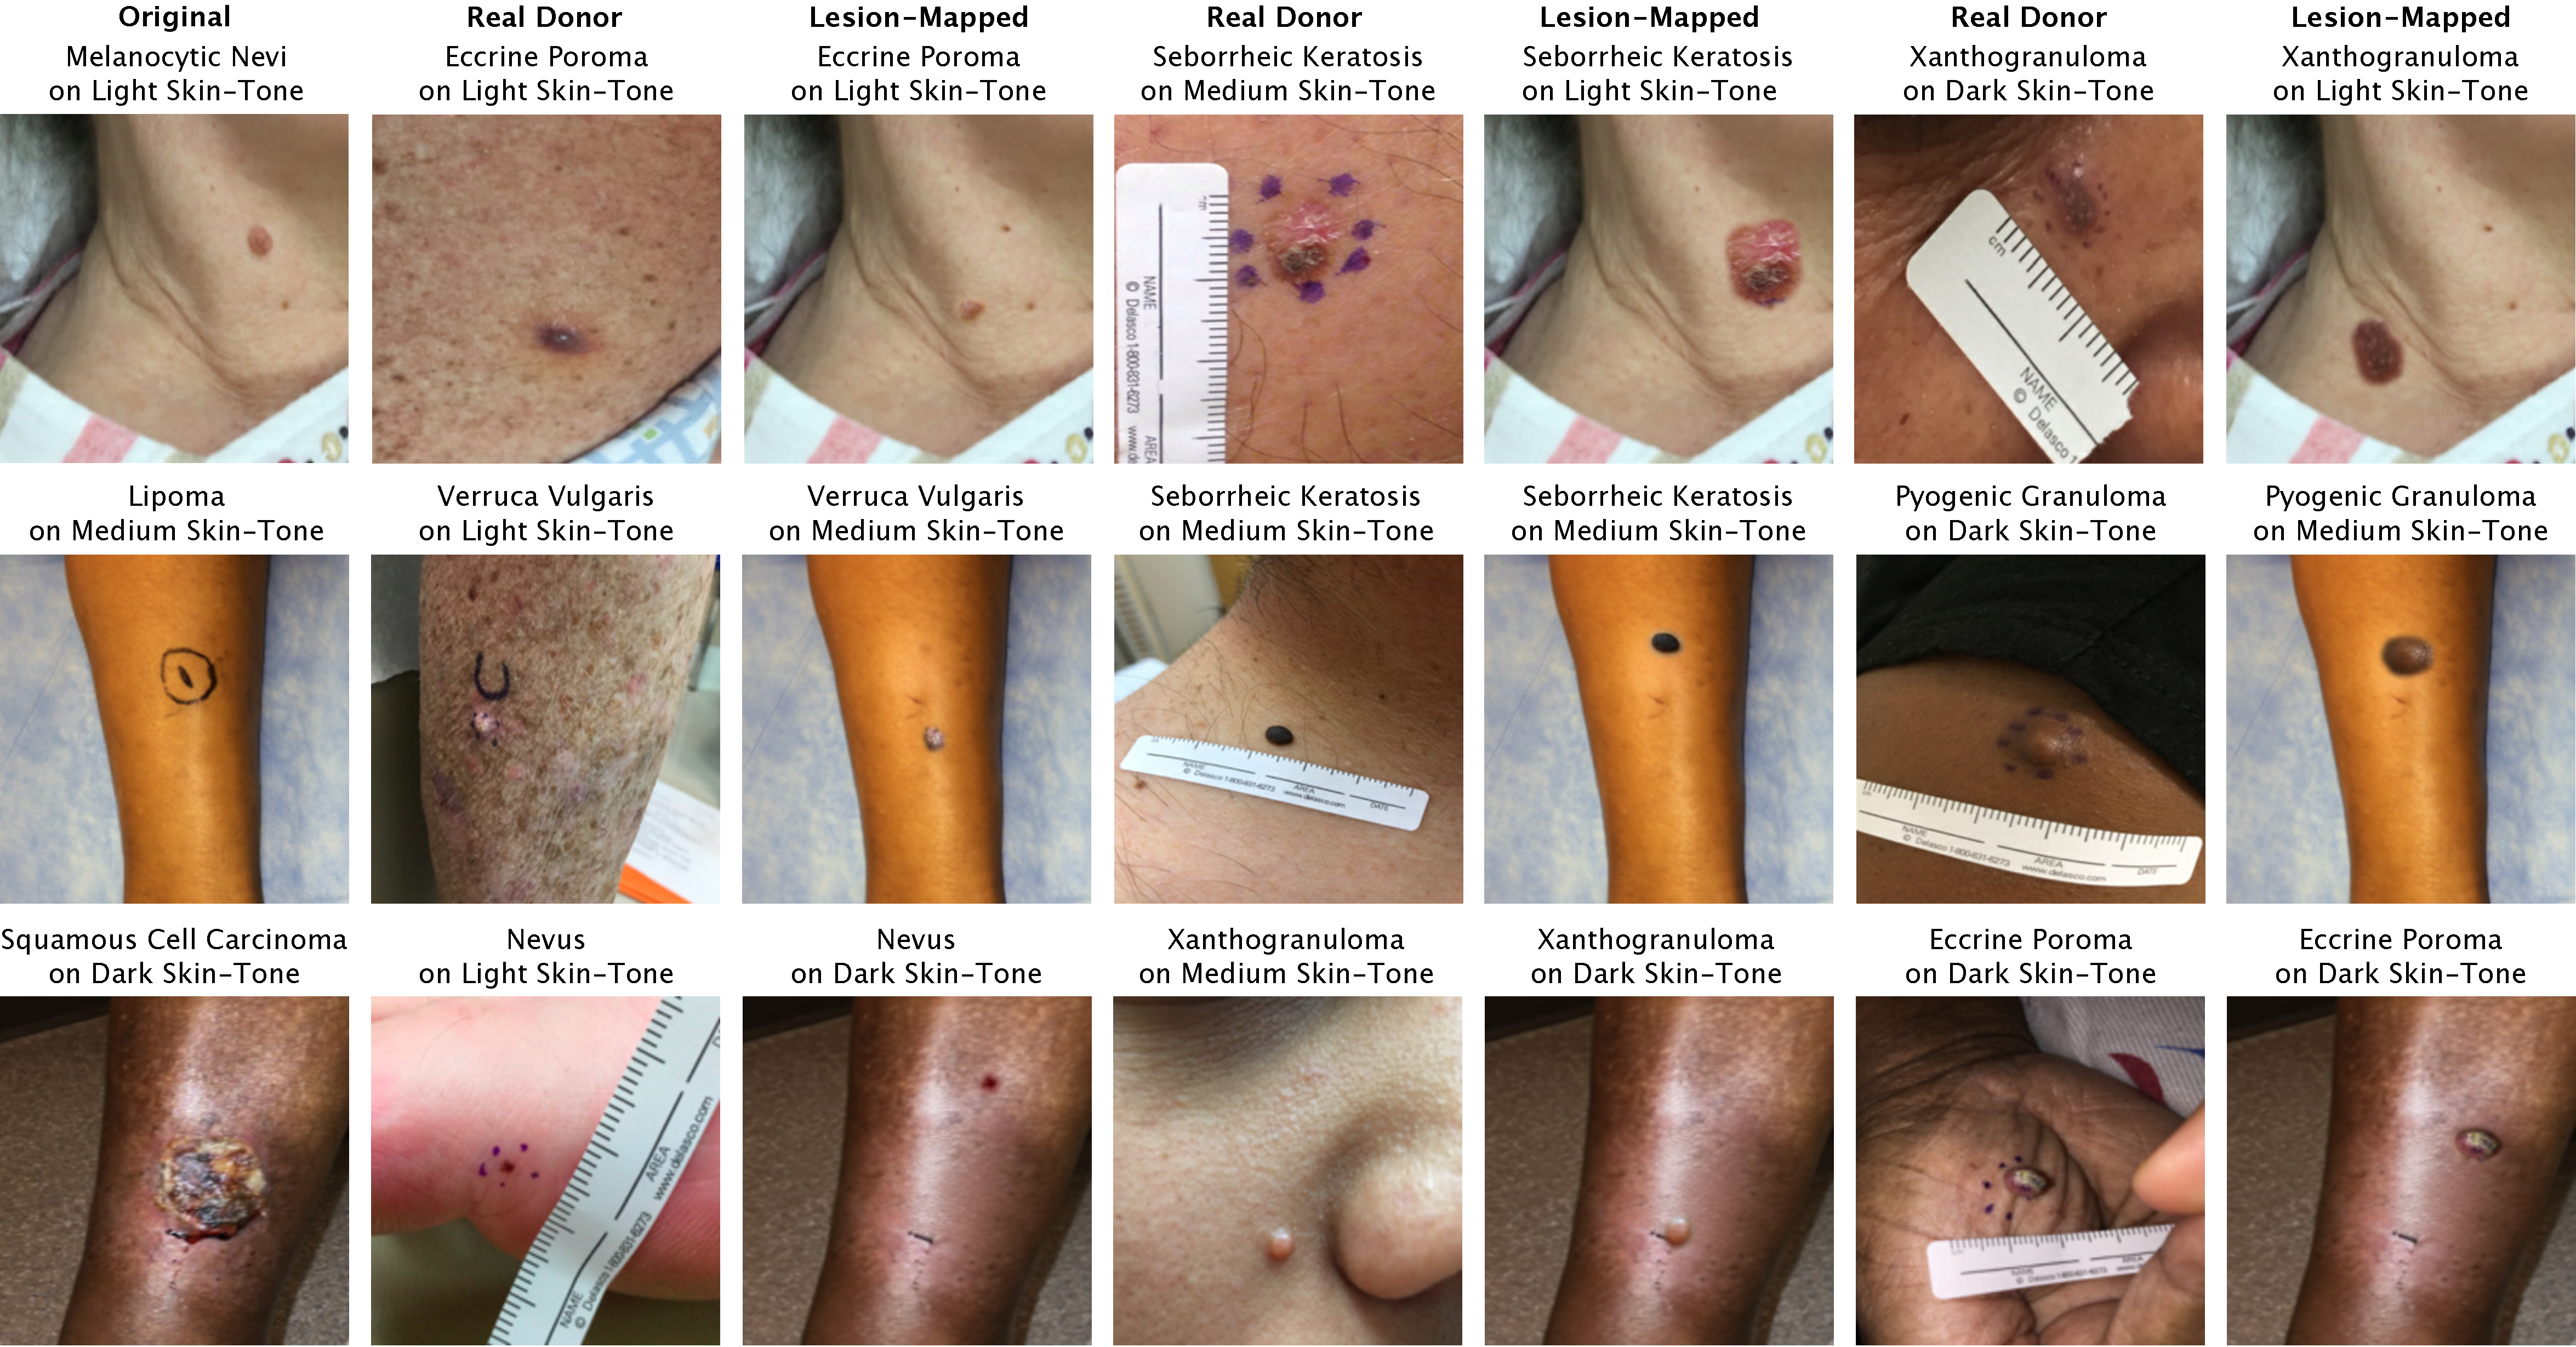
\includegraphics[width=1\linewidth]{cgDDI/cgddi_lesion_mapped_2.pdf}
   \caption{\textbf{Accepted Lesion-Mapped Synthetics}. Further visualization of samples that passed algorithmic constraints.}
   \label{cgddi:fig:lm_2}
\end{figure}

\paragraph{Lesion-Mapped Synthetics}
\label{cgddi:sec:discard_mapping}
Since we generate 80,427 lesion-mapped synthetics, a manual review of the full set was not possible. We did, however, algorithmically eliminate any output images that did not meet the 10-pixel padding criterion, which should avoid strange placements and lighting, as previously mentioned. Given 309 synthetic healthy images, 334 sDDI masks, and a single iteration loop, following the description given in Section \ref{cgddi:sec:lesion_mapping}, it is possible to generate 103,206 synthetics. However, the algorithmic constraint discards 22,779 samples (or 22\%) of possible samples. We show additional lesion-mapped samples, along with their real donors, in Figure \ref{cgddi:fig:lm_2}.

\paragraph{Semantic Synthetics}
\label{cgddi:sec:semantic_discard}
As we generate 185,400 semantic synthetics, a manual review of the full set was not possible. However, we ablate generation quality for random subsets of the data, along with their corresponding amounts of training data. We observe that at around 10 training samples, image quality becomes viable. This is visualized in Figure \ref{cgddi:fig:sample_ablation}.

Some observations of synthetics with fewer than 10 training samples include: 
\begin{enumerate}
    \item Unrealistic skin texture.
    \item Anatomical inconsistencies.
    \item Unrealistic or unnatural patterns in lesion appearance or placement.
    \item Ruler or other generative artifacts.
    \item Poor instruction following.
\end{enumerate}

Given this criterion, do not include semantic synthetics produced with $\leq 10$ training samples in our classification experiments. This means that of the 185,400 samples, we include 60,255 (about 33\%) in the classification experiments. We do, however, publish all semantic synthetics regardless of their original number of training samples for further research and evaluation.


\subsection{Results and Discussion}

\subsubsection{Experimental Setup}

This section provides detailed information about our classification experiments, including model architecture, training hyperparameters, data-splitting strategy, fairness metric computation, and statistical analysis.

\paragraph{Model Architecture and Training Hyperparameters}
For our classification experiments, we followed the contrastive disentanglement approach from \cite{du_2023_fairdisco} and incorporated the patch-alignment improvements from \cite{aayushman-2024}. The classifier architecture consists of a Vision Transformer (ViT-B/16) pre-trained on ImageNet-21k. The PatchAlign training pipeline (which we use as the baseline) already applies a standard augmentation stack --- random crops, rotations, color jitter, horizontal flips, and ImageNet normalization. cgDDI gains are therefore reported \emph{on top of} this stack and operate along axes orthogonal to conventional augmentation: skin tone, lesion morphology, and single-sample disease coverage cannot be synthesized by pixel-level transforms.

Regarding hyperparameters, we follow \cite{aayushman-2024}. Adam optimizer with learning rate $1e^{-4}$, with a linear decay scheduler at step size 2 and a decay factor of 0.8. Batch size is set to 32, and training runs for a total of 20 epochs.

For Experiment 2 (fine-tuning on real data), we used a lower learning rate of $1e^{-5}$ and trained for an additional 20 epochs with early stopping.

The baseline model (referred to as ``Baseline" in Table \ref{cgddi:perf_table}) uses a pre-trained ResNet-18 as the feature extractor and only cross-entropy loss on the final labels for optimization, following the approach described in \cite{aayushman-2024}. We compare our method against this baseline and FairDisCo \cite{du_2023_fairdisco}.

\paragraph{Data Splits and Leakage Prevention}
To ensure valid evaluation and prevent data leakage, we carefully designed our experimental setup. For all experiments, we used the same 80/20 train/test split as in previous work \cite{du_2023_fairdisco, aayushman-2024} when evaluating on the DDI dataset, enabling direct comparison with baseline methods.

For Experiment 1 (training exclusively on synthetic data), we utilized synthetic images from our cgDDI dataset, ensuring no overlap with test images from the real DDI dataset. This is accomplished by removing any lesion-mapped synthetics which are generated from image donors present on the test set (as split by the \cite{aayushman-2024} seeds). Furthermore, we remove any semantic synthesis generated using a target disease and a healthy image prompt, which together reconstruct an image present in the test set.

For Experiment 2 (fine-tuning on real data), we first trained the model on our synthetic cgDDI dataset, then fine-tuned it on the real DDI training set. The model was evaluated on the same real DDI test set as in Experiment 1 and as \cite{aayushman-2024}.

\paragraph{Test-set subgroup composition}
For transparency under the small-data regime, we report per-skin-tone test counts. DDI 5-fold cross-validation yields an average of 131 test samples per fold (42 Light I--II, 48 Medium III--IV, 41 Dark V--VI). The F17k 15\% hold-out has 55 total (22 Light, 17 Medium, 16 Dark). These small absolute sample sizes are inherent to biopsy-confirmed, skin-tone-balanced dermatology data; we treat them as a structural constraint of the field and encourage further data collection with verified Fitzpatrick labels.

\paragraph{Statistical Significance}
To assess the statistical robustness of our results, and to directly compare against \cite{aayushman-2024} we performed five experiments with differnet train/test split seeds. These are taken directly from \cite{aayushman-2024} code repository and are ['S36' 'S37', 'S38', 'S39', 'S40'], which we believe to be seeds 36, 37, 38, 39, and 40. We calculated the mean performance and standard deviation for each metric. The standard deviations reported in Table~\ref{cgddi:perf_table} reflect the variation across these splits.

\subsubsection{Classification and Fairness Metrics}

\label{cgddi:sec:cls}\label{cgddi:sec:cls_fairness}
We assess the quality of our synthetic data by running malignancy classification experiments on real data. For classifier design, we follow the contrastive disentanglement approach from \cite{du_2023_fairdisco} and incorporate the patch-alignment improvements from \cite{aayushman-2024}. Keeping the same classifier design and training method allows us to directly measure the benefit of our generation framework and synthesized data. We evaluate on the same DDI benchmark as \cite{du_2023_fairdisco, aayushman-2024}, and report the same fairness metrics, which we formalize next.




The fairness metrics used in our evaluation are: PQD, DPM, and EOM. In brief, PQD measures the prediction quality difference between each skin tone group as a ``best vs worst" ratio measurement, similar to IR. DPM computes the percentage diversity of positive outcomes for each skin tone group, and this percentage increases as we reach similar positive prediction rates across populations. EOM measures true-positive rate consistency, which increases as skin tone groups have similar true-positive rates. Formally:

\noindent
\begin{align}
\mathrm{PQD} &= \frac{\min_{k\in S}\mathrm{acc}_k}{\max_{k\in S}\mathrm{acc}_k} & 
\mathrm{DPM} &= \frac{1}{|\mathcal{C}|}\sum_{c\in\mathcal{C}}\frac{\min_{k\in S}p\bigl(\hat y = c \mid s=k\bigr)}{\max_{k\in S}p\bigl(\hat y = c \mid s=k\bigr)}
\end{align}

\noindent
\begin{equation}
\mathrm{EOM}
\;=\;
\frac{1}{|\mathcal{C}|}
\sum_{c\in\mathcal{C}}
\frac{\min_{k\in S}p\bigl(\hat y = c \mid y=c,\,s=k\bigr)}
     {\max_{k\in S}p\bigl(\hat y = c \mid y=c,\,s=k\bigr)}
\end{equation}

Where $\mathcal{C} = \{\mathrm{benign},\mathrm{malignant}\}$, $y$ is the ground truth and $\hat{y}$ is the model prediction.

\begin{table}
  \caption{\textbf{Malignancy Classification and Fairness Performance.} Abbreviations: ``R." denotes real data, ``S." denotes synthetic data, ``R. + S." denotes a combination of both.}
  \label{cgddi:perf_table}
  \centering
  \scriptsize
  \setlength\tabcolsep{4pt}
  \resizebox{\linewidth}{!}{%
  \begin{tabular}{lccccccc}
    \toprule
      & \multicolumn{4}{c}{\textbf{Accuracy (\%)} $\pm$ Std‐dev.}
      & \multicolumn{3}{c}{\textbf{Fairness} $\pm$ Std‐dev.}       \\
    \cmidrule(lr){2-5} \cmidrule(lr){6-8}
    Method 
      & Mean & Light & Medium & Dark 
      & PQD  & DPM   & EOM   \\
    \midrule
    Baseline (R.)
      & $82.4\pm1.5$ & $83.3\pm1.0$ & $74.6\pm5.7$ & $89.7\pm2.2$
      & $77.0\pm1.9$ & \underline{$75.2$} $\pm13.3$ & $58.7\pm4.3$ \\
    FairDisCo (R.)
      & $83.8\pm0.4$ & $88.6\pm0.1$ & $71.7\pm2.2$ & $92.0\pm2.8$
      & $78.0\pm4.5$ & $72.8\pm12.0$               & $63.7\pm3.5$ \\
    PatchAlign (R.)
      & \underline{$87.4$} $\pm1.2$ & \underline{$89.6$} $\pm2.6$
      & $80.3\pm5.7$ & \underline{$92.3$} $\pm1.3$
      & $86.9\pm6.1$ & $74.9\pm12.0$               & $69.6\pm1.7$ \\
    \midrule
    Exp. 1 (S. only)
      & $86.4\pm1.0$ & $88.9\pm1.5$ & \underline{$84.1$} $\pm2.6$& $86.0\pm1.8$
      & $\mathbf{94.6}$ $\pm3.1$ & $\mathbf{82.0}$ $\pm9.7$& \underline{$81.9$} $\pm2.8$ \\
    Exp. 2 (R. + S.)
      & $\mathbf{90.9}$ $\pm1.3$ & $\mathbf{93.3}$ $\pm2.2$ & $\mathbf{86.4}$ $\pm4.1$ & $\mathbf{93.0}$ $\pm1.0$
      & \underline{$92.5$} $\pm2.5$ & $68.8\pm11.3$& $\mathbf{86.6}$ $\pm1.9$\\
    \bottomrule
  \end{tabular}%
  }
\end{table}

\paragraph{Malignancy classification.}
We run two experiments: \textit{Experiment 1:} Training purely on synthetic data generated by the cgDDI framework, and \textit{Experiment 2:} Training on synthetic data and then fine-tuning on a subset of real DDI data. Evaluations for both experiments are performed on holdout test sets of real DDI images. This is visualized in Figure \ref{cgddi:fig:cgddi_framework}, color-coded as red. To avoid data leaks, we exclude training on synthetics conditioned on samples from the test set. We also avoid semantic synthetics generated with $\leq 10$ training samples.

We find that \textit{Experiment 1} (training on synthetic cgDDI data) achieves a mean accuracy similar to the prior methods from \cite{du_2023_fairdisco,aayushman-2024}, while improving in fairness metrics. In \textit{Experiment 2} (training on synthetic data and fine-tuning on real images), we achieve higher accuracy across all skin tone categories. Results of both experiments are shown in Table \ref{cgddi:perf_table}. 

As stated in \cite{aayushman-2024}, EOM is the most important fairness metric, and \textit{Experiment 2} achieves the highest EOM score among all the baseline methods, followed by \textit{Experiment 1}. This improvement in the EOM metric demonstrates the essential role of synthetic data from cgDDI in the training regimen. We also observed that the PQD metric is slightly lower in \textit{Experiment 2} than in \textit{Experiment 1}, as the real-data performance gains appear to be greater for light and dark skin tones than for medium. This could be due to disease imbalances found in the real data. While DPM decreases in \textit{Experiment 2}, we note that the metric can increase with false positives, as noted by \cite{aayushman-2024}.

\subsubsection{Disease Rarity Performance}

To understand how synthetic augmentation affects disease classification performance across varying training data availability, we stratify performance by disease frequency. We define common diseases as those represented by more than 10 observations (107 test cases), rare as between 3 and 10 (19 test cases), and very rare as between 1 and 2 (6 test cases).

We observe that fine-tuning on real data improves the common case, slightly reduces the rare case, and has no impact on the very rare case. As discussed, our synthetic dataset contains significantly more observations of rare diseases than the base DDI, while the intricacies and imbalance of real data encourage the model to improve performance on common cases (leading to a higher mean accuracy), as shown in Table~\ref{cgddi:tab:rare_disease}. Notably, our lesion-mapping approach enables augmentation for single-sample diseases, maintaining competitive accuracy even for conditions with minimal training data.

\paragraph{Generative fairness metrics.}
While classification fairness metrics demonstrate improved equity in malignancy diagnosis, we additionally evaluate whether our generation methods maintain quality parity across skin tones. We compute Fréchet Inception Distance (FID) \cite{heusel-2017}, Kernel Inception Distance (KID) \cite{binkowski-2018}, and Learned Perceptual Image Patch Similarity (LPIPS) \cite{zhang2018perceptual} between cgDDI and held-out real DDI images.

All three metrics demonstrate reasonable stability across skin tones, with low dispersion for FID ($\sigma = 8.39$, max/min ratio = 1.22) and LPIPS ($\sigma = 0.011$, max/min ratio = 1.04). KID shows the largest relative spread ($\sigma = 0.010$, max/min = 2.41), but the absolute differences are small, so the practical impact is limited. Each metric slightly favors a different tone (FID: Medium best, KID: Dark best, LPIPS: Light best), indicating no systematic advantage for any population. This is shown in Table~\ref{cgddi:tab:gen_fairness}. We further ablate these metrics per generative method in the Appendix, along with additional visual examples that reinforce generative fairness across populations.

\begin{table}[t]
\centering
\caption{Classification accuracy stratified by disease rarity.}
\label{cgddi:tab:rare_disease}
\begin{tabular}{lcc}
\toprule
\multicolumn{1}{c}{Disease} & Exp.~1 (S) & Exp.~2 (S+R) \\
Commonality & Accuracy (\%) & Accuracy (\%) \\
\midrule
Common ($>$10)  & 85.05 & 91.59 \\
Rare (3--10)    & 94.74 & 89.47 \\
V.\ Rare (1--2) & 83.33 & 83.33 \\
\bottomrule
\end{tabular}
\end{table}

\begin{table}[t]
\centering
\caption{Generative quality per skin tone: FID, KID, and LPIPS between cgDDI synthetics and held-out real DDI images.}
\label{cgddi:tab:gen_fairness}
\begin{tabular}{lccc}
\toprule
Skin Tone & FID $\downarrow$ & KID $\downarrow$ & LPIPS $\downarrow$ \\
\midrule
Light   & 103.45 & 0.039 & 0.715 \\
Medium  &  88.41 & 0.032 & 0.741 \\
Dark    & 108.07 & 0.016 & 0.734 \\
\midrule
Max/Min &   1.22 & 2.41  & 1.04  \\
\bottomrule
\end{tabular}
\end{table}

\subsubsection{Contribution of Each Generation Method}

\paragraph{Contribution of Generation Methods}

We evaluate the individual contribution of each generation method to classification performance by training models on different subsets of cgDDI.

\begin{table}[h]
\centering
\caption{Ablation study: Classification performance using different synthetic data subsets.}
\label{cgddi:tab:ablation}
\begin{tabular}{lcccc}
\toprule
Training Data & Mean Acc. & Light & Medium & Dark \\
\midrule
Real DDI only & 82.4 & 83.3 & 74.6 & 89.7 \\
Healthy + Lesion-mapped & 81.2 & 82.1 & 78.4 & 82.9 \\
Semantic only & 84.7 & 86.3 & 82.5 & 85.2 \\
All cgDDI (Exp. 1) & 86.4 & 88.9 & 84.1 & 86.0 \\
\bottomrule
\end{tabular}
\end{table}

Training solely on healthy and lesion-mapped synthetics slightly reduces overall performance compared to training solely on DDI (-1.2\% mean accuracy); however, it does increase performance on medium skin tone. We believe this is likely due to the limited appearance distribution of non-lesion image features (body location, lighting conditions, skin tone, etc.) and the still relative imbalance bias originating from the base dataset toward medium skin tone in the lesion-mapped synthetics. Semantic synthetics, however, provide a strong individual contribution (+2.3\% mean accuracy) and a positive boost across all skin tones, likely due to parametric learning of disease-specific features. The combination of all three methods yields the best overall performance, growing the training distribution and validating our multi-pronged approach. These results are shown in Table \ref{cgddi:tab:ablation}.

\paragraph{Generative Quality by Method}

We provide detailed quality metrics for each generation method in the same way as in the main text via FID, KID and LPIPS. We now discuss performance per generative method:

\paragraph{Lesion-mapped (non-parametric):} This method achieves the strongest distributional alignment, with the best mean FID (79.73) and best mean KID (0.003). Its LPIPS (0.698) matches Healthy data. Variability across tones is moderate (FID $\sigma = 12.28$; KID $\sigma = 0.002$), consistent with the methods design for rare diseases.

\paragraph{Healthy:} These metrics come in second in FID (mean 102.48) and KID (mean 0.010), while LPIPS is strong (0.698), matching Lesion-mapped in perceptual similarity. Tone-wise variability is modest for KID ($\sigma = 0.001$) and larger for FID ($\sigma = 13.35$), suggesting broadly similar behavior across tones with some room to improve distributional alignment.

\paragraph{Semantic (parametric):} This approach shows the most tone consistency on FID ($\sigma = 4.10$) but has the weakest absolute FID (mean 130.52) and KID (mean 0.054). LPIPS is higher (0.746) than the other methods, indicating lower perceptual similarity. Semantic generation shows consistency across tones, despite being fully parametric, while having the largest divergence from the base dataset as a learned and sampled approach.

Detailed results are shown in Table \ref{cgddi:tab:quality_by_method}. These metrics complement our classification fairness results in Tables \ref{cgddi:perf_table}, 3 and the visual qualitative results throughout the paper. Additionally, this supports that cgDDI maintains equitable generation quality across populations.

\begin{table}[h]
\centering
\caption{FID, KID, and LPIPS scores stratified by generation method and skin tone.}
\label{cgddi:tab:quality_by_method}
\begin{tabular}{llcccc}
\toprule
Metric & Method & Light & Medium & Dark & $\sigma$ \\
\midrule
\multirow{3}{*}{FID $\downarrow$} 
& Healthy & 94.02 & 92.11 & 121.33 & 13.35 \\
& Lesion-mapped & 72.75 & 69.46 & 96.99 & 12.28 \\
& Semantic & 134.67 & 124.94 & 131.95 & 4.10 \\
\midrule
\multirow{3}{*}{KID $\downarrow$}
& Healthy & 0.012 & 0.008 & 0.010 & 0.001 \\
& Lesion-mapped & 0.005 & 0.003 & 0.001 & 0.002 \\
& Semantic & 0.055 & 0.069 & 0.037 & 0.013 \\
\midrule
\multirow{3}{*}{LPIPS $\downarrow$}
& Healthy & 0.703 & 0.692 & 0.700 & 0.005 \\
& Lesion-mapped & 0.703 & 0.692 & 0.698 & 0.005 \\
& Semantic & 0.738 & 0.756 & 0.743 & 0.008 \\
\bottomrule
\end{tabular}
\end{table}

% Lesion-mapped synthetics achieve the best distributional alignment (lowest FID/KID), while semantic generation shows the most consistency across skin tones (lowest $\sigma$ for FID).

\subsubsection{Generalization to Fitzpatrick17k}

% %%%%%%%%%%%%%%%%%%%%%%%%%%% REBUTTAL CONTENT %%%%%%%%%%%%%%%%%%%%%%%%%%%%%%%%%

\begin{figure}[t]
  \centering
  \includegraphics[width=1\linewidth]{cgDDI/f17k_inpaint.pdf}
   \caption{\textbf{Fitzpatrick17k Algorithmic Masking and Healthy Sampling}. We expand our work to other datasets, which may not include lesion and skin masks. Masks are generated using an off-the-shelf segmentation model.}
   \label{cgddi:fig:f17k_in}
\end{figure}

We discuss additional real datasets relevant to our study in Section \ref{cgddi:sec:related}, particularly F17k, the most commonly cited macroscopic dataset for training and evaluating fairness in dermatological AI. However, we note that F17k is skin-tone-unbalanced and annotated by non-experts without biopsy or histopathological evidence, leading to more than $30\%$ label noise \cite{groh_2021_evaluating}. To evaluate the generalizability of our method and to demonstrate mask-free processing, while reducing these concerns, we run the full cgDDI framework on a verified subset of F17k \cite{groh-2024}.

This dataset totals 364 samples: 143 light-skinned, 113 medium-skinned, and 108 dark-skinned. The samples cover eight main diseases: atopic dermatitis, cutaneous T-cell lymphoma, dermatomyositis, lichen planus, Lyme disease, pityriasis rosea, pityriasis rubra pilaris, and secondary syphilis. Only cutaneous T-cell lymphoma is malignant and overlaps with DDI. We begin processing this data by generating masks with an off-the-shelf segmentation algorithm.

\paragraph{Automated Segmentation Masks}
\label{cgddi:samv3}

When processing the DDI dataset, we opt to use pre-made, expert-verified segmentation masks \cite{carrion-2023} because they are readily available for this dataset. However, when processing other datasets, this sort of additional information may not be included. We mention in Section \ref{cgddi:sec:in-painting} that our framework is compatible with algorithmically generated masks, and, in this section, we demonstrate this functionality by leveraging the Segment Anything 3 (SAMv3) model \cite{carion2025sam3segmentconcepts}. We elect this model as a generalist segmentation algorithm proof of concept; we acknowledge that other methods, particularly those tailored to dermatology, might perform equally well or better.

% \begin{itemize}
%     \item \textbf{Valid skin lesion segmentation:} SAMv3 successfully segments lesions across skin tones without dataset-specific training.
%     \item \textbf{Healthy skin regions:} After healthy image generation, SAMv3 identifies normal skin regions for lesion mapping.
%     \item \textbf{Quality control:} We apply confidence thresholding to filter low-quality masks and manually verify the output for an additional dataset.
% \end{itemize}

\paragraph{Healthy Synthetics: F17k}

We perform a segmentation inference pass using SAMv3 to predict ``rash'' areas with a confidence cutoff of $0.35$. Subsequently, we input these masks into Section \ref{cgddi:sec:in-painting} of our framework as-is, producing healthy F17k synthetics that will serve the rest of our pipeline. As with DDI, we manually verify all generated healthy samples and retain those that pass the discard criteria outlined in Section \ref{cgddi:ref:healthy_discard}. After review, 46 verified healthy samples are kept: 21 light-skinned, 16 medium-skinned, and 9 dark-skinned. This discard rate is higher than that for DDI; we believe this is due to imperfect masks, which lead to more artifacts. Results for this and Section \ref{cgddi:samv3} are shown in Figure \ref{cgddi:fig:f17k_in}.

\begin{figure}[t]
  \centering
  \includegraphics[width=1\linewidth]{cgDDI/f17k_semantic_mapped.pdf}
   \caption{\textbf{Fitzpatrick17k Semantic and Lesion-Mapped Synthetics}. Semantic sampling captures the intricacies differentiating these two related diseases as we LoRA fine-tune separate models per-disease, while mapping extends the views for each real lesion.}
   \label{cgddi:fig:f17k_sem_map}
\end{figure}

\paragraph{Lesion-Mapped Synthetics: F17k}
\label{cgddi:sec:mapped_f17k}

We perform a second segmentation inference pass, using SAMv3 to delineate the ``skin'' area of our synthetic healthy samples with a confidence cutoff of $0.35$. The aforementioned lesion masks and these new skin masks are passed into Section \ref{cgddi:sec:lesion_mapping} of our pipeline as-is. The discard criteria described in Section \ref{cgddi:sec:discard_mapping} are applied (46.9\% discard rate), leading to 1,124 new lesion-mapped synthetics: 529 light-skinned, 373 medium-skinned, 222 dark-skinned samples. The larger imbalance observed here is largely due to F17k skin-tone distribution and the resulting healthy synthetic output distribution.

\paragraph{Semantic Synthetics: F17k}

We now randomly sample 85\% of the verified F17k dataset to learn text-inversion tokens for each condition, then fine-tune generative models using LoRA and prior preservation via healthy synthetics, following Section \ref{cgddi:sec:parametric}. The remaining 15\% of the data is held out for classifier testing and is balanced across skin tones. Relevant to the minimum training data and discard criteria outlined in Section \ref{cgddi:sec:semantic_discard}, all 8 main conditions in F17k contain more than 10 training samples. We then sample 690 semantic synthetics per condition (46 healthy images x 3 skin tones x 5 samples), for a total of 5,520 new images, equally split across skin tones (1,840 each). Results for this and Section \ref{cgddi:sec:mapped_f17k} are shown in Figure \ref{cgddi:fig:f17k_sem_map}.

\paragraph{Classification Fairness: F17k}

We repeat classification experiments using the PatchAlign \cite{aayushman-2024} method described in Section \ref{cgddi:sec:cls} and compute the fairness metrics shown in Section \ref{cgddi:sec:cls_fairness}. These experiments are tested on the held-out F17k data described above. We first train a baseline model using the same classifier algorithm and training parameters on real data (specifically, the 85\% used above to train the generative models). This baseline method reaches 86.0\% classification accuracy. We then train from the same initialization but purely on F17k lesion-mapped and semantic synthetics, achieving 88.4\% mean accuracy (up 2.4\%), with a rise in medium skin-tone accuracy, which is offset by lower dark-skin accuracy, offset by lower dark-skin accuracy, while fairness metrics remain relatively close. We then take this checkpoint and fine-tune on real data, and we observe that mean accuracy rises another 2.3\% to 90.7\%, leading or tied for per-skin-tone accuracy across all skin tones. PQD is also the highest here, and while DPM is lower than the baseline method, \cite{aayushman-2024} argues that PQD is the most important metric, while DPM can be skewed by false positives as discussed in the main text. These results are shown in Table \ref{cgddi:tab:f17k-f17k}.

% Table for F17k-trained models on F17k test set (add baseline)
\begin{table}[h]
\centering
\caption{F17k-trained models evaluated on the F17k test set. Baseline is trained on real data.}
\label{cgddi:tab:f17k-f17k}
\resizebox{\textwidth}{!}{%
\begin{tabular}{llccccccc}
\toprule
\textbf{Setting} & \textbf{Method} & \textbf{Acc} & \textbf{Light} & \textbf{Med} & \textbf{Dark} & \textbf{PQD} & \textbf{DPM} & \textbf{EOM} \\
\midrule
\multirow{3}{*}{F17k $\rightarrow$ F17k} 
 & Baseline & 86.0\% & 86.7\% & 82.4\% & \textbf{90.9\%} & 0.906 & \textbf{0.455} & 0.500 \\
 \cmidrule(l){2-9}
 & Synth Only & 88.4\% & 86.7\% & \textbf{94.1\%} & 81.8\% & 0.869 & 0.441 & 0.500 \\
 & Synth + Real & \textbf{90.7\%} & 86.7\% & \textbf{94.1\%} & \textbf{90.9\%} & \textbf{0.921} & 0.441 & 0.500 \\
\bottomrule
\end{tabular}}
\end{table}

\subsubsection{Cross-Dataset Validation}

In this section, we emphasize cross-data framework compatibility by mapping and sampling synthetics using a combination of inputs from both F17k and DDI datasets.

\paragraph{Cross-Dataset Lesion Mapping}

\begin{figure}[t]
  \centering
  \includegraphics[width=1\linewidth]{cgDDI/bidirection_mapping.pdf}
   \caption{\textbf{Bidirectional Lesion-Mapping}. We leverage our method as-is to map lesions from one dataset to the other and vice versa.}
   \label{cgddi:fig:bi_mapping}
\end{figure}

We demonstrate lesion-mapping generalizability through bidirectional cross-dataset synthesis. In this case, we show effective mapping of lesions from DDI to F17k and vice versa. This does not require any additional processing or changes other than swapping the source and target sample directories. The resulting synthetics are visualized in Figure \ref{cgddi:fig:bi_mapping}. The resulting totals after the discard criteria outlined in Section \ref{cgddi:sec:discard_mapping} are shown in Table \ref{cgddi:tab:cross-mapping}. Given that DDI is more balanced across skin tones, we see a tighter distribution when mapping to it than to F17k.

\begin{table}[h]
\centering
\caption{Cross-dataset Lesion-Mapping}
\label{cgddi:tab:cross-mapping}
\begin{tabular}{lcccc}
\toprule
\textbf{Direction} & \textbf{Total} & \textbf{Light} & \textbf{Medium} & \textbf{Dark} \\
\midrule
DDI lesions $\rightarrow$ F17k healthy & 13,822 & 6,593 & 4,267 & 2,962 \\
F17k lesions $\rightarrow$ DDI healthy & 9,394 & 3,103 & 3,272 & 3,019 \\
\bottomrule
\end{tabular}
\end{table}

\paragraph{Cross-Dataset Semantic Generation}
Similarly, we leverage the previously trained generative models to sample new synthetics using cross-dataset healthy images as prompts. Note that these models are not retrained (as there is little disease overlap between the datasets) but are simply re-prompted with new image samples. Table \ref{cgddi:tab:cross-semantic} displays the total number of new semantic synthetics. As skin-tone sampling here is controlled via textual prompts, we can sample equally across target skin tones.

\begin{table}[h]
\centering
\caption{Cross-dataset Semantic Sampling}
\label{cgddi:tab:cross-semantic}
\begin{tabular}{lcc}
\toprule
\textbf{Configuration} & \textbf{Total Images} & \textbf{Per Skin Tone} \\
\midrule
F17k diseases + DDI healthy prompts & 37,080 & 12,360 \\
DDI diseases + F17k healthy prompts & 8,970 & 2,990 \\
\bottomrule
\end{tabular}
\end{table}

%==============================================================================
\paragraph{Cross-dataset Classification Experiments}
%==============================================================================
To exhaustively test the cross-dataset classification capabilities of models trained individually and in combination, we run extensive experiments that report overall accuracy, per-skin-tone accuracy, and fairness metrics across various configurations, using the base classifier we have used throughout the paper, based on \cite{aayushman-2024}.

Table \ref{cgddi:tab:cross-transfer} shows the performance of F17k-trained models on fully unseen DDI data and DDI-based model performance on fully unseen F17k data. Note that when testing a DDI-trained model on F17k or vice versa,, or vice versa, the limited overlap between diseases might indicate that the model has not generalized well to unseen disease classes. This leads to the first F17k baseline classifier obtaining higher accuracy but lower fairness metrics. When training on DDI synthetics, however, the richer, larger, balanced, and more diverse set of synthetics generalizes significantly better to unseen F17k data.


\begin{table}[h]
\centering
\caption{Cross-dataset transfer performance, a model is trained on one dataset, then evaluated on the other's test set. The baseline model is trained solely on real data.}
\label{cgddi:tab:cross-transfer}
\resizebox{\textwidth}{!}{%
\begin{tabular}{llccccccc}
\toprule
\textbf{Setting} & \textbf{Method} & \textbf{Acc} & \textbf{Light} & \textbf{Med} & \textbf{Dark} & \textbf{PQD} & \textbf{DPM} & \textbf{EOM} \\
\midrule
\multirow{3}{*}{F17k $\rightarrow$ DDI} 
 & Baseline & \textbf{79.6\%} & \textbf{64.3\%} & \textbf{82.2\%} & \textbf{87.5\%} & 0.735 & 0.500 & 0.500 \\
 \cmidrule(l){2-9}
 & Synth Only & 74.3\% & 57.1\% & 77.8\% & 82.5\% & 0.693 & 0.604 & 0.440 \\
 & Synth + Real & 75.2\% & \textbf{64.3\%} & 80.0\% & 77.5\% & \textbf{0.804} & \textbf{0.678} & \textbf{0.703} \\
\midrule
\multirow{3}{*}{DDI $\rightarrow$ F17k} 
 & Baseline & 60.5\% & 66.7\% & 47.1\% & 72.7\% & 0.647 & 0.515 & 0.526 \\
 \cmidrule(l){2-9}
 & Synth Only & \textbf{74.4\%} & \textbf{80.0\%} & \textbf{70.6\%} & 72.7\% & \textbf{0.882} & 0.556 & \textbf{0.613} \\
 & Synth + Real & 69.8\% & 73.3\% & 76.5\% & 54.5\% & 0.713 & \textbf{0.664} & 0.388 \\
\bottomrule
\end{tabular}}
\end{table}

% % Table for F17k models on DDI test set (cross-dataset transfer)
% \begin{table}[h]
% \centering
% \caption{F17k models evaluated on DDI test set (cross-dataset transfer). Baseline is trained solely on real data.}
% \label{cgddi:tab:f17k-ddi}
% \begin{tabular}{lccccccc}
% \toprule
% \textbf{Method} & \textbf{Acc} & \textbf{Light} & \textbf{Med} & \textbf{Dark} & \textbf{PQD} & \textbf{DPM} & \textbf{EOM} \\
% \midrule
% F17k Baseline & \textbf{79.6\%} & 64.3\% & \textbf{82.2\%} & \textbf{87.5\%} & 0.735 & 0.500 & 0.500 \\
% \midrule
% F17k Synth Only & 74.3\% & 57.1\% & 77.8\% & 82.5\% & 0.693 & 0.604 & 0.440 \\
% F17k Synth + Real & 75.2\% & 64.3\% & 80.0\% & 77.5\% & \textbf{0.804} & \textbf{0.678} & \textbf{0.703} \\
% \bottomrule
% \end{tabular}
% \end{table}

\paragraph{Aggregated Cross-Dataset Training}
We also train on a mixed collection of both datasets, baseline using only real data, using purely synthetics, and also fine-tuning those checkpoints on real imagery. Table \ref{cgddi:tab:combined} presents the complete aggregated results. We train on the full combination of DDI and F17k synthetics, including within-dataset lesion-mapped and semantic samples as well as cross-dataset variants from Tables \ref{cgddi:tab:cross-mapping} and \ref{cgddi:tab:cross-semantic}, then fine-tune on the aggregated real training data from both sources. We observe that the synthetics and real data generally outperform other settings, highlighting the value of data augmentation using our methods.

\begin{table}[h]
\centering
\caption{Aggregated cross-dataset performance. The baseline model is trained on mixed real data.}
\label{cgddi:tab:combined}
\resizebox{\textwidth}{!}{%
\begin{tabular}{llccccccc}
\toprule
\textbf{Setting} & \textbf{Method} & \textbf{Acc} & \textbf{Light} & \textbf{Med} & \textbf{Dark} & \textbf{PQD} & \textbf{DPM} & \textbf{EOM} \\
\midrule
\multirow{3}{*}{Mix $\rightarrow$ F17k} 
 & Baseline & 86.0\% & 86.7\% & 88.2\% & 81.8\% & \textbf{0.927} & \textbf{0.471} & 0.500 \\
 \cmidrule(l){2-9}
 & Synth Only & 86.1\% & \textbf{93.3\%} & 88.2\% & 72.7\% & 0.779 & 0.378 & \textbf{0.750} \\
 & Synth + Real & \textbf{93.0\%} & \textbf{93.3\%} & 88.2\% & \textbf{100.0\%} & 0.882 & 0.378 & 0.500 \\
\midrule
\multirow{3}{*}{Mix $\rightarrow$ DDI} 
 & Baseline & 83.2\% & 75.0\% & 82.2\% & 90.0\% & 0.833 & \textbf{0.679} & 0.784 \\
 \cmidrule(l){2-9}
 & Synth Only & 79.7\% & 71.4\% & 84.4\% & 80.0\% & 0.846 & 0.436 & \textbf{0.833} \\
 & Synth + Real & \textbf{86.7\%} & \textbf{82.1\%} & \textbf{84.4\%} & \textbf{92.5\%} & \textbf{0.888} & 0.600 & 0.750 \\
\bottomrule
\end{tabular}}
\end{table}


\subsubsection{Discussion of Cross-Dataset Experiments}

The cross-dataset experiments demonstrate several key properties of the cgDDI framework.

\textbf{Pre-made segmentation masks are not necessary.} We observe that out-of-the-box segmentation algorithms are capable of fair and accurate masks, which are then directly compatible with the cgDDI framework. Using pixel-perfect, verified masks might reduce the discard rate, but this trade-off is likely worth it for the scalability of algorithmically generated masking.

\textbf{Effective cross-dataset transfer.} Lesion-mapping algorithms and generative models can be effectively leveraged across datasets, leading to higher diversity synthetics which lead to improved classifier performance downstream. For example, training exclusively on real F17k data, we achieve 86.0\% accuracy, adding synthetics from our method raises this metric to 90.7\%, while finally mixing in DDI synthetics achieves 93.0\%.

\textbf{Improved fairness through dataset aggregation.} We observe that the leading PQD score includes our synthetics in five out of six experiments. The only exception is a large mix of real training data, which highlights the persistent value of clean, high-quality real samples. 

\textbf{Knowledge transfer despite minimal disease overlap.} Only one condition (cutaneous T-cell lymphoma) appears in both DDI and the verified F17k subset. Nevertheless, cross-dataset training improves performance on both benchmarks, suggesting the model learns generalizable features about skin lesion appearance rather than dataset-specific patterns.


\subsubsection{Applicability to Additional Datasets}

\label{cgddi:sec:generalization}

Our framework's design principles are dataset-agnostic and applicable to any medical imaging domain with segmentation masks:

\paragraph{Component Transferability}
\begin{itemize}
    \item \textbf{Inpainting Pipeline:} Compatible with any medical images where lesion removal is meaningful (dermatology, ophthalmology, radiology)
    \item \textbf{Lesion Mapping:} Generalizes to any scenario requiring transplantation of pathological regions between images
    \item \textbf{Parametric Generation:} Standard diffusion fine-tuning applicable to any labeled collection with $\geq$10 samples
\end{itemize}

\paragraph{Domain-Specific Considerations}
While we validate on dermatology due to its unique fairness challenges and data availability, adaptation to other domains requires:
\begin{enumerate}
    \item Segmentation masks (manual or automated via SAM/DINO)
    \item Fairness-relevant metadata (demographics, equipment type, acquisition parameters)
    \item Domain expertise for quality assessment
\end{enumerate}

\paragraph{DDI Selection}
We selected DDI over other datasets due to their (1) lack of biopsy confirmation leading to unreliable ground truth (F17k), (2) absence of dermatologist-verified skin-tone labels (SCIN) needed for fairness evaluation, (3) the dermoscopic setting being relatively unrepresentative of clinical practice in very low resource communities (HAM1000) (4) the ready availability of segmentation masks for DDI (sDDI) and (5) computational constraints preventing exhaustive cross-dataset experiments within the review period. Due to these limitations growing the complexity of further experiments on other datasets, we leave these experiments as future work.

\subsubsection{Limitations}

\label{cgddi:sec:limits}

While our experiments demonstrate that cgDDI improves classification performance and fairness while reducing dataset size limitations, extremely efficient parametric training and generation (fewer than 10 samples) remain an open challenge in the vision community, and even more so for medical AI. We identify promising directions for further reduction:

\begin{itemize}
    \item \textbf{Few-shot adaptation}: Techniques like Model-Agnostic 
    Meta-Learning (MAML) could potentially reduce requirements to 3-5 samples
    \item \textbf{Further prompt engineering}: Advanced prompt design might enable 
    zero-shot generation for unseen diseases, such as explicitly describing in natural language visual features associated with particularly rare morphologies
    \item \textbf{Cross-disease transfer}: Learning shared disease 
    characteristics could enable better generalization
\end{itemize}

We leave systematic investigation of these approaches as future work, noting that our non-parametric lesion mapping already enables augmentation from single samples. Additionally, our approach provides generative control via prompting. However, instruction following is strongly influenced by sampling hyperparameters. Our parameter selection, while informed by preliminary experiments, was not exhaustively optimized due to computational costs. Finally, while we manually and algorithmically review generated samples, incorporating dermatologist review across all our subsets would help assess dataset quality and inform filtering.

\subsubsection{Summary}

We present cgDDI, a novel hybrid generation framework that solves the technical challenge of synthesizing fair and diverse dermatological imagery under extreme data constraints. A key contribution in combining non-parametric lesion mapping (enabling 300$\times$ augmentation of single-sample diseases) with parametric generation (achieving high-fidelity synthesis from just 10 samples). Additionally, the method can generate in-distribution healthy images, which are later leveraged by the pipeline. This approach maintains quality parity across skin tones while providing fine-grained semantic control for both common and rare diseases.

The method's effectiveness is validated through large-scale data synthesis and extensive experiments: models trained purely on our synthetic data achieve competitive accuracy and state-of-the-art performance when fine-tuned on real data. Additionally, we measure generative fairness by low disparity between skin tones and strong performance on very rare diseases. By successfully growing a small but clean medical base dataset, we demonstrate that careful algorithmic design can overcome severe data bias and limitations in medical AI and potentially other data-constrained domains. We further discuss generalizability in the Appendix, noting that although we leverage DDI for its unique properties, all components of our design are applicable to other datasets.


% ============================================================
% Chapter 5 — Monocular Metric 3D Reconstruction (DermDepth)
% ============================================================
\chapter{Monocular Metric 3D Reconstruction for Dermatology}\label{section:dermdepth}

HealNet, FEDD, and cgDDI (Chapters~\ref{section:healnet}--\ref{section:cgddi}) addressed three different facets of the data-scarcity problem in dermatology --- temporal label scarcity, single-image label scarcity with fairness evaluation, and demographic and rare-disease imbalance --- but all three operate entirely in 2D appearance space. Clinical assessment of skin lesions, however, is fundamentally a three-dimensional measurement problem: the $E$ in ABCDE screening (Asymmetry, Border, Color, Diameter, Elevation) literally requires depth; lesion volume tracking requires a metric scale; and surface-morphology features such as ulceration and scaling are 3D-textural by definition. Existing dermatological 3D capture relies on plenoptic cameras or time-of-flight scanners that are unavailable in low-resource clinics. Meanwhile, natural-image monocular depth estimation has advanced rapidly with foundation models, but whether they generalize to dermatological-scale regimes remains unknown. This chapter answers that question: we benchmark four foundation depth models on three dermatological datasets, find systematic $4$--$156\times$ scale errors, and show that a small scale and normal head trained on a synthetic 3D dermoscopic dataset corrects these errors without disturbing the foundation model's relative geometry --- realising the same frozen-backbone + small-head + synthetic-data + fairness-stratification pattern that powered the earlier chapters, now in 3D.

\section{DermDepth - Toward Monocular Metric Scale 3D Reconstruction Models for Dermatology}\label{section:dermdepth_abs}

Dermatological practice routinely involves measuring and tracking lesion size, morphology, and texture, as critical components of wound or skin cancer screening, monitoring, and diagnosis. To accomplish this task, practitioners often image the skin surface with commonly available off-the-shelf camera sensors. This has led to an overwhelming research focus on 2D methods, while these objectives naturally benefit from 3D information. In this work, we demonstrate that dense monocular 3D reconstructions, metric-scale measurements, and rich surface-normal texture estimates are achievable for both dermoscopic and macroscopic cases without additional hardware or multiple captures. We present \textbf{DermDepth}, the first single-view, metric-scale 3D model for the dermatological domain, and \textbf{D-Synth}, the first synthetic dermoscopic dataset with pixel-perfect 3D information. Our experiments show that training DermDepth on D-Synth corrects metric-scale error from over $16\times$ to under $1.1\times$ on real dermoscopic data, while preserving geometric quality and increasing texture richness. Fine-tuning on a small amount of real clinical samples generalizes our method across three real-world benchmarks spanning the few mm to hundred cm range, diverse skin-tones, chronic wound cases, and produces measurements broadly consistent with disease size reported in medical literature.

\subsection{Background and Related Work}\label{sec:dd_intro}

Skin lesions and chronic wound conditions impact the lives of millions of patients all over the world, with an estimated 3 billion people lacking access to adequate dermatological care, especially in poor communities \cite{coustasse_2019_use}. Non-melanoma skin cancer is the most common malignant tumor, with its incidence increasing year over year, and melanoma cancers are highly accretive, meaning morphology undergoes progressive growth \cite{wang-2024-cancer}. Early detection significantly increases survival rates \cite{balch-2009}, emphasizing the scale and importance of active ABCDE measurements in dermatology \cite{blum-2003}; features that AI algorithms could facilitate tracking.

\begin{figure}[t]
    \centering
    \includegraphics[width=\textwidth]{DermDepth/DD_1.pdf}
    \caption{\textbf{D-Synth Dataset.} Rendered skin-lesion synthetics from our D-Synth pipeline with dense pixel-perfect 3D information and texture normal maps.}
    \label{fig:D-Synth}
\end{figure}

As such, dermatology is often a measurement problem: clinicians screen, triage, and monitor lesions or wounds by tracking changes in size, border irregularity, surface morphology, and texture over time \cite{argenziano-1998}. These characteristics are inherently 3D, yet standard point-of-care information capture remains 2D imaging, likely due to the cost and inaccessibility of 3D systems. Critically, these measurements require scale consistency, ideally in metric space. 2D images are sometimes paired with rulers. However, clinically valuable information such as elevation, indentation, or surface roughness is missed by simple width estimates. This observation closes a loop on directions foreshadowed in the advancement work of Chapters~\ref{section:healnet} and~\ref{section:fedd}, where the need for integrated, scale-consistent image-based dermatological monitoring was already identified as a key future goal.

The primary bottleneck toward training and evaluating 3D AI methods in dermatology is the difficulty of collecting suitable datasets \cite{xie-2025}. Purpose-built devices have enabled limited 3D dermatological capture: SKINL2 \cite{de-faria-2019} provides dermoscopic depth via plenoptic camera and WoundsDB \cite{juszczyk-2020} captures clinical wounds via time-of-flight, demonstrating significant downstream benefits: increased classification accuracy ($\uparrow$10\%), sensitivity ($\uparrow$29\%) \cite{pereira-2021}, and $3\times$ more accurate area estimation \cite{juszczyk-2020}, but require special hardware. Existing monocular approaches are limited to coarse elevation classification \cite{abhishek2024lesion}, relative-scale defocusing \cite{parekh-2024}, or multi-view private-data methods \cite{zhang-2025}. Synthetic dermatological data \cite{sinha2024dermsynth3d,kim-2024} has been explored for 2D tasks but not for metric 3D depth.

Meanwhile, natural-image monocular depth estimation has advanced rapidly through the use of large vision transformers \cite{oquab2023dinov2}. Recent methods claim metric depth output: MoGe-2 \cite{wang2025moge2} and MapAnything \cite{keetha2026mapanything} predict scale via decoupled heads, Depth Anything v3 \cite{depthanything3} uses canonical camera transformations, and Pixel-Perfect Depth \cite{xu2025pixel} refines depth via diffusion generation. Whether these models generalize to dermatological images remains underexplored. In order to address these challenges, we present the following contributions:

\begin{enumerate}
    \item \textbf{D-Synth}, a novel rendered synthetic dataset leveraging knowledge-informed lesion growth models \cite{kim-2024}, contributing pixel-perfect 3D depth in metric scale, surface normals, and camera intrinsics, as shown in Figure~\ref{fig:D-Synth}.

    \item \textbf{DermDepth}, a model and fine-tuning approach for affine-invariant 3D prediction methods, correcting metric scale error across benchmarks by up to a factor of 14$\times$, while improving surface normal detail and performing equitably across Fitzpatrick skin tones (disparity: 10.9~$\rightarrow$~1.02).

    \item \textbf{Systematic evaluation} of metric scale accuracy on dermatological images across 4 foundation models, 3 evaluation datasets, and 2 imaging modalities.

    \item \textbf{Downstream validation} of metric accuracy for 3D lesion measurement (area, width, volume) from single photographs, validated against ruler ground truth and literature review.
\end{enumerate}

\subsection{Dataset}\label{sec:dd_datasets}

\begin{table}[t]
\centering
\caption{\textbf{DermDepth Datasets.} SKINL2 is stratified by version, WoundsDB by patient, and DDI by Fitzpatrick skin tone.}
\label{tab:dd_datasets}
\small
\setlength\tabcolsep{4pt}
\begin{tabular}{@{}l l r r r l@{}}
\toprule
Dataset & Modality & Total & Train & Test & GT source \\
\midrule
D-Synth  & Synth.\ dermoscopy & 4{,}000 & 3{,}000 & 1{,}000   & Rendered depth \\
SKINL2   & Dermoscopy         &     375 &     263 & 112   & Plenoptic camera \\
WoundsDB & Clinical wound     &      77 &      50 &  27   & ToF sensor \\
DDI      & Clinical + ruler   &      47 &      33 &  14   & Ruler annotation \\
\bottomrule
\end{tabular}
\end{table}

\subsubsection{D-Synth}
We extend \cite{kim-2024}, which generates dermoscopic-style samples following biologically motivated lesion growth patterns. Originally, the method was designed to export 2D images and binary masks; we additionally contribute functionality to export per-pixel depth on a metric scale, camera intrinsics, and normal maps, while also adding camera angles and multiple lesions. We synthesize 4{,}000 samples across 131 melanin levels and 240 lesion morphologies at 12--20\,mm distance with $75^\circ$ field of view. We call this new dataset D-Synth (Figure~\ref{fig:D-Synth}). D-Synth retains the anatomical realism stack from \cite{kim-2024}, including layered melanosome, blood, and lipid models across the epidermis, dermis, and hypodermis, alongside physics-based light scatter spanning multiple wavelengths and skin tones. D-Synth's principal value, however, is not photorealism but the availability of pixel-perfect 3D ground truth (metric depth, surface normals, and camera intrinsics) at scale --- a training signal that is not obtainable from real dermatological capture in any reliable form. The remaining sim-to-real RGB-appearance gap is closed by the progressive real-data refinement described in Section~\ref{sec:training}, and the design choice is empirically validated in Table~\ref{tab:dd_main}, where D-Synth alone already drives the dominant SKINL2 correction $16.1\!\times\!\rightarrow\!1.11\!\times$ while preserving SI-$\delta_1$ at 100\%.

\subsubsection{SKINL2 and WoundsDB}\label{sec:realdata}
To bridge the sim-to-real gap and evaluate across clinical distances, we process SKINL2 and WoundsDB for metric-scale training and evaluation. SKINL2 plenoptic depth maps exhibit local planar noise \cite{lourenco-2022}, and WoundsDB time-of-flight maps are often sparse, low-resolution, with spatial offset from the RGB sensor. These issues may introduce noise into geometric evaluation, but do not affect the metric scale.

\subsubsection{DDI}\label{sec:dd_ddi}
DDI \cite{daneshjou_2022_disparities} is a fairness-focused 2D dataset akin to smartphone-captured images during first-pass clinical examination, positioned between SKINL2 and WoundsDB in terms of sampling distance. This dataset is collected without 3D information; however, we find 47 samples include a fully visible medical ruler with known dimensions \cite{delasco} and matching segmentation masks \cite{carrion-2023}. This allows us to estimate the metric scale of the scene and evaluate fairness across skin tones. Table~\ref{tab:dd_datasets} summarises all datasets and their train/test splits.

\subsection{Method}\label{sec:dd_method}

\subsubsection{Base Architecture}\label{sec:architecture}
MoGe-2 and Pixel-Perfect Depth \cite{wang2025moge2,xu2025pixel} predict affine-invariant depth maps, which can then be scaled to metric space. This metric scaling factor is predicted via dedicated output heads by both MoGe-2 and MapAnything \cite{keetha2026mapanything}, with the former also able to predict normal maps via a dedicated convolutional head. Given that real dermatology data sources may have an accurate scale but noisy depth (and thus normals), we elect MoGe-2 as our base architecture due to its design flexibility.

Let $M$ denote the full model predicting depth $\hat{d} = M(I)$ for image $I$. On dermatological inputs, we observe $\hat{d} \approx s \cdot d^*$ where $d^*$ is the true depth, $s \gg 1$ for dermoscopy and $s < 1$ for clinical photography at intermediate distances. The relative structure, however, is preserved: $\hat{d}_i / \hat{d}_j \approx d^*_i / d^*_j$. Since only the scalar $s$ is incorrect, the fix is localized to the scale head, which motivates our decision to freeze the backbone and fine-tune only the scale prediction head (and optionally the normal head).

\subsubsection{Training Strategy}\label{sec:training}
When training on D-Synth, we freeze the backbone encoder and fine-tune the scale and normal output heads. The scale head is composed of a 3-layer Multi-Layer Perceptron (MLP) that takes the CLS token from the base encoder as input and outputs a single scalar in log-space. The scale factor is then multiplied by the predicted affine-invariant point cloud to convert from relative to metric units. The loss is thus defined as:

\begin{equation}
    \mathcal{L}_{\text{scale}} = \left(\log \hat{s} - \log s^*\right)^2
\end{equation}

\noindent Where $\hat{s}$ is the predicted scale factor and $s^*$ is the ground-truth value. This formulation makes the loss symmetric with respect to over- or under-estimation, which is useful since the monocular scale can be ambiguous. The normal output head is composed of a ConvStack \cite{wang2025moge2} decoder, similar to the 3D head, that inputs feature maps and outputs a 3-channel per-pixel normal vector that is L2-normalized to unit length. The normal loss formula is:

\begin{equation}
\mathcal{L}_{\text{normal}} = \frac{1}{HW} \sum_{i} \angle(\hat{\mathbf{n}}_i, \mathbf{n}_i^*)^2
\end{equation}

\noindent Where $H, W$ are image dimensions, $\hat{\mathbf{n}}_i$ and $\mathbf{n}_i^*$ are the predicted and ground-truth unit surface normals at pixel $i$, and $\angle(\cdot,\cdot)$ denotes the angle in radians between two vectors. When training on SKINL2, WoundsDB, or DDI, given their noisy depth and normal maps, we also freeze the normal output head.

We split the datasets 70\% for training and 30\% for testing, stratified across versions for SKINL2, patient cases for WoundsDB (so that no patient appears in both splits), and skin tones for DDI. We train for 1{,}000 steps with a learning rate of $10^{-4}$, the AdamW optimizer, and a batch size of 4 on a single A100 GPU. An exponential moving average (EMA, decay 0.999) is applied to all parameters; we find EMA essential for stable convergence, as raw checkpoints exhibit oscillations and overcorrection. The same protocol is used for real-data training stages, with learning rate reduced to $5 \times 10^{-5}$ and 2{,}000 steps per stage.

\subsubsection{DDI Fairness and Lesion Measurements}\label{sec:downstream}
We estimate lesion width, area and volume for held-out DDI samples with visible rulers for validation. Given the predicted metric depth and estimated camera intrinsics, we back-project to a 3D point cloud and compute surface area via cross-product triangle integration, lesion width as the major PCA axis, and volume as the integral over the region bounded by the lesion surface and a fitted boundary plane. These measurements scale quadratically (area) or cubically (volume) with depth, introducing depth error that makes accurate scale predictions important. We then compare against estimated ground-truth measurements derived from the manually segmented ruler area and literature review. We ablate these results per Fitzpatrick skin tone to measure fairness.

\subsection{Results and Discussion}\label{sec:dd_results}

\begin{table}[t]
\centering
\caption{\textbf{Scale Results.} Foundation models systematically miss scale on dermatological data despite strong geometry (SI-$\delta_1$). DermDepth fine-tunes only 2.1\,M parameters (0.6\,\%), with significant scale correction on all benchmarks. Scale ratio target is $1.0\times$; DDI ratio target is $1.0\times$. \DDS{}: synthetic data only. Eval on held-out test sets.}
\label{tab:dd_main}
\small
\setlength\tabcolsep{4.5pt}
\begin{tabular}{@{}l c cc cc c@{}}
\toprule
\multirow{2}{*}{Method} & \multirow{2}{*}{Params} & \multicolumn{2}{c}{SKINL2 (dermoscopy)} & \multicolumn{2}{c}{WoundsDB (clinical)} & DDI \\
\cmidrule(lr){3-4} \cmidrule(lr){5-6} \cmidrule(lr){7-7}
& & Scale~$r$ & SI-$\delta_1$\,(\%) & Scale~$r$ & SI-$\delta_1$\,(\%) & Ratio~$\rho$ \\
\midrule
DA3~\cite{depthanything3}          & 1.4\,B  & 4.16  & 99.6 & 0.67 & 89.1 & 53.6 \\
MapAnything~\cite{keetha2026mapanything} & 1.1\,B  & 10.88 & 99.3 & \underline{0.75} & 80.7 & 156.1 \\
PPD~\cite{xu2025pixel}       & 831\,M  & 16.21 & 92.0 & 0.66 & \underline{91.3} & 90.4 \\
MoGe-2~\cite{wang2025moge2}         & 331\,M  & 16.10 & \underline{100.0} & 0.62 & 91.1 & 81.0 \\
\midrule
\DDS{}   & \textbf{2.1\,M\,ft} & \textbf{1.11}  & \underline{100.0} & 0.28 & 91.1 & \underline{9.2} \\
\textbf{DermDepth}     & \textbf{2.1\,M\,ft} & \underline{0.87} & \underline{100.0} & \textbf{0.91} & \textbf{92.6} & \textbf{1.95} \\
\bottomrule
\end{tabular}
\end{table}

\begin{figure}[t]
    \centering
    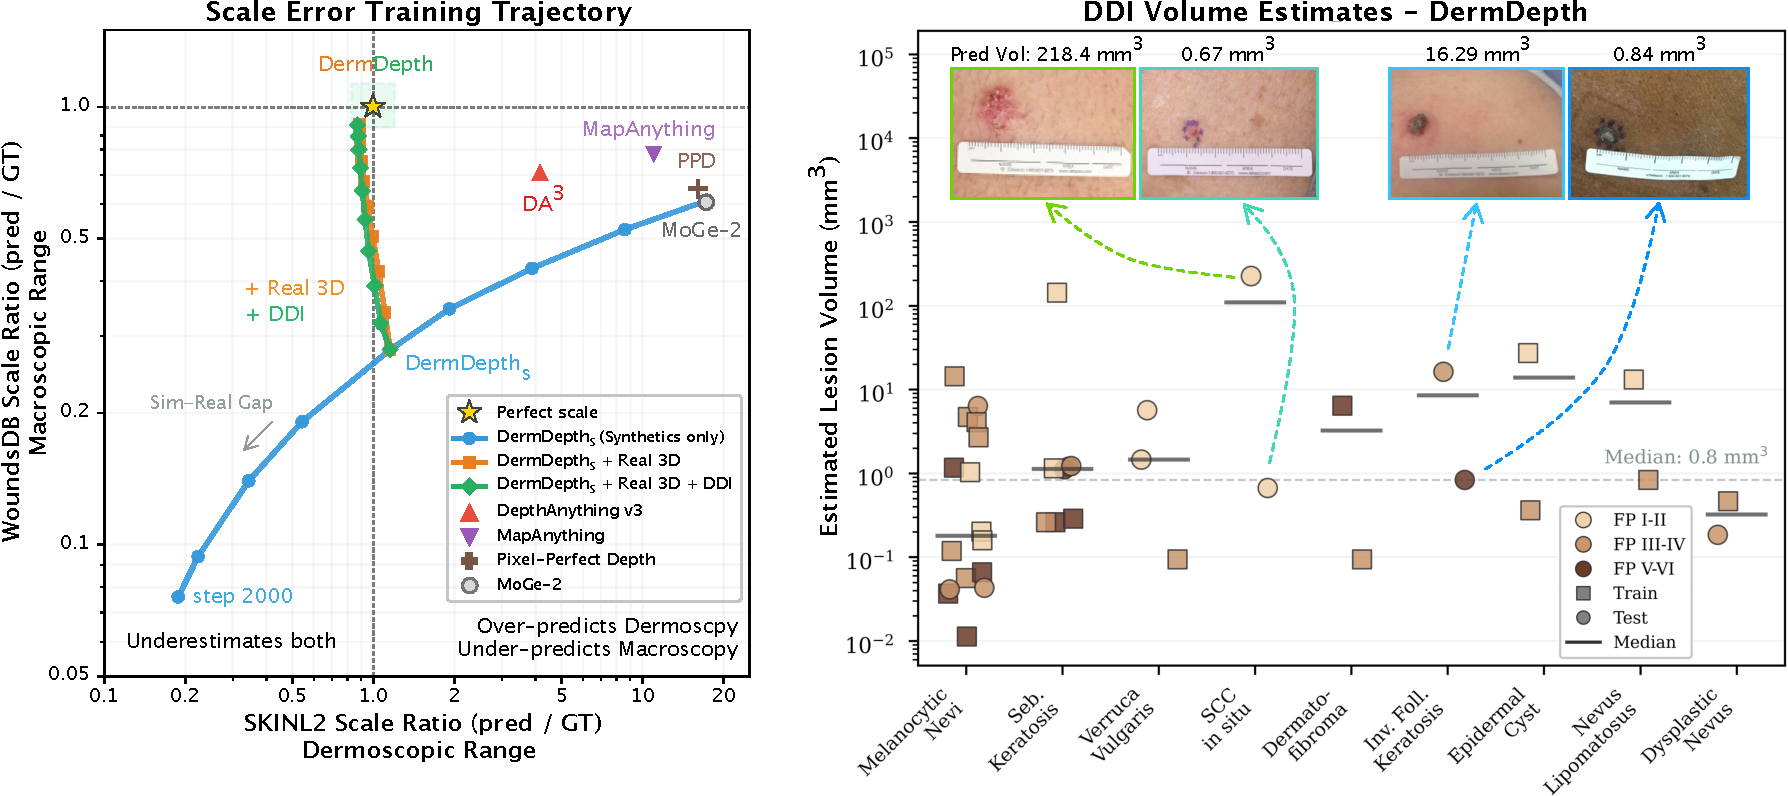
\includegraphics[width=\textwidth]{DermDepth/DD_2Bold.pdf}
    \caption{\textbf{Scale Correction Training (Left), Predicted Volume (Right).} We measure dermoscopic range (cm-level) over-estimation and macroscopic range (m-level) underestimation for all foundation models tested. Training on D-Synth corrects dermoscopic error, and adding real data corrects macroscopic error (left). We demonstrate DermDepth volume measurements on DDI held-out test data (right).}
    \label{fig:dd_quantitative}
\end{figure}

\begin{figure}[t]
    \centering
    \includegraphics[width=\textwidth]{DermDepth/DD_3Bold.pdf}
    \caption{\textbf{Predicted Depth, Scale, and Normals.} We visualize performance across three datasets at different metric distances. We find DermDepth produces more accurate and consistent scale and normal maps with finer lesion detail. We note that DDI was not collected alongside 3D information; we estimate scale error from the known ruler area. The ground-truth depth references themselves carry dataset-specific sensor noise (SKINL2 plenoptic local planar noise; WoundsDB time-of-flight sparsity and RGB-misalignment, as discussed in Section~\ref{sec:realdata}), so visual differences between GT and DermDepth in the figure should be interpreted with these artifacts in mind. The scale-aligned SI-$\delta_1$ in Table~\ref{tab:dd_main} quantifies geometry agreement at 100\% (SKINL2) and 92.6\% (WoundsDB) --- per-pixel depth ratio within 1.25$\times$ of GT.}
    \label{fig:dd_comparison}
\end{figure}

\subsubsection{Baseline Methods and Metrics}
We benchmark four recent models that claim metric depth output: \textbf{Depth Anything~3} \cite{depthanything3} (DA3-METRIC-LARGE; 1.4\,B params), \textbf{MapAnything} \cite{keetha2026mapanything} (1.1\,B), \textbf{Pixel-Perfect Depth} \cite{xu2025pixel} (PPD; 831\,M, diffusion refinement with MoGe-2 scaling as done on the official codebase), and \textbf{MoGe-2} \cite{wang2025moge2} (331\,M).

We report three complementary metrics: \textbf{Scale ratio} $r = \text{median}(\hat{d}_i / d_i^*)$, where $r{=}1.0$ is perfect; \textbf{SI-$\delta_1$} = percentage of pixels where the scale-aligned depth ratio falls within $[1/1.25,\, 1.25]$, measuring geometry quality independent of global scale; and \textbf{DDI ratio} $\rho = A_{\text{pred}} / A_{\text{GT}}$, measuring predicted ruler area relative to the known ruler area of $6.6\,\text{cm}^2$.

\subsubsection{Experimental Results}\label{sec:dd_main_results}

Table~\ref{tab:dd_main} demonstrates that every evaluated foundation model produces systematically incorrect metric scale on dermatological images. All four baselines overestimate dermoscopic depth by $4$--$16\times$ (SKINL2) and underestimate clinical wound depth at $0.6$--$0.75\times$ (WoundsDB), with DDI ruler-area ratios ranging from $54\times$ to $156\times$. Crucially, geometry quality is high across all models (SI-$\delta_1 \geq 92\%$), confirming that the 3D structure is captured correctly and supporting our decision to freeze the majority of parameters while focusing on scale and normal map training.

PPD internally uses MoGe-2 for metric grounding and consequently inherits near-identical scale bias ($16.2\times \approx 16.1\times$ on SKINL2), while its diffusion refinement slightly degrades geometry (SI-$\delta_1$: 92.0\% vs.\ 100.0\%). DA3, despite having the most parameters, overestimates by $4.2\times$.

DermDepth corrects scale across all three benchmarks. With synthetic data alone, SKINL2 scale drops from $16.1\times$ to $1.11\times$ while high-quality geometry is preserved (SI-$\delta_1${=}100\% and SI-AbsRel{=}0.017). With progressive real-data training, DermDepth achieves $0.87\times$ on SKINL2, $0.91\times$ on WoundsDB, and $1.95\times$ on DDI, bringing all three benchmarks close to metric scale, as shown in Figure~\ref{fig:dd_quantitative} (left).

\subsubsection{Ablation: What and How Much to Fine-Tune}\label{sec:dd_ablation}

This subsection re-enables experiments that were cut from the conference submission due to page limits. Table~\ref{tab:dd_ablation} presents two ablation axes: \emph{how much of the model} to fine-tune (capacity) and \emph{what data} to use (progressive refinement).

\begin{table}[t]
\centering
\caption{\textbf{Ablation: model capacity and data composition.} Rows~1--4: increasing trainable parameters worsens scale \emph{and} geometry. Rows~2, 5--6: progressive real data corrects residual distance bias. Scale target is $1.0\times$.}
\label{tab:dd_ablation}
\small
\setlength\tabcolsep{4pt}
\begin{tabular}{@{}l ccc cc@{}}
\toprule
 & \multicolumn{3}{c}{Scale ratio $r$ ($\to 1.0$)} & \multicolumn{2}{c}{SI-$\delta_1$ (\%)} \\
\cmidrule(lr){2-4} \cmidrule(lr){5-6}
Configuration & SKINL2 & WoundsDB & DDI & SKINL2 & WoundsDB \\
\midrule
Baseline (MoGe-2)                 & 16.10 & 0.62 & 81.0 & 100.0 & 91.1 \\
\rowcolor{green!6}
Scale head, synth                  & \textbf{1.11}  & 0.28 &  9.2 & 100.0 & 91.1 \\
+ Decoder, synth                   & 0.14  & 0.06 & 0.76 &  99.9 & 85.8 \\
+ Full model, synth                & 0.09  & 0.04 & 0.13 &  99.8 & 77.5 \\
\midrule
Scale head, +\,real depth          & \textbf{0.89}  & \textbf{0.92} & 18.3 & 100.0 & 91.1 \\
\rowcolor{green!6}
\textbf{Scale head, +\,DDI pseudo} & \underline{0.87}  & \underline{0.91} & \textbf{1.95} & \textbf{100.0} & \textbf{92.6} \\
\bottomrule
\end{tabular}
\end{table}

\paragraph{Model capacity (rows~2--4).}
Starting from the synthetic-only setting, we compare training the scale head alone (2.1\,M), adding the decoder (22\,M), and the full model (326\,M). Increasing capacity is strictly harmful: the decoder overcorrects SKINL2 to $0.14\times$ and WoundsDB to $0.06\times$ (inverting the original errors), while degrading geometry (WoundsDB SI-$\delta_1$: 91.1\% $\to$ 85.8\%) and collapsing DDI to $0.76\times$. Full-model fine-tuning is worse still: $0.09\times$ on SKINL2, $0.04\times$ on WoundsDB, $0.13\times$ on DDI, with severe geometry loss (77.5\%). This occurs because 3{,}000 synthetic samples are insufficient to re-learn 22--326\,M decoder parameters; the domain gap between synthetic and real data leads to overfitting, catastrophic forgetting, and overcorrection in the opposite direction.

\paragraph{Data composition (rows~2, 5--6).}
Synthetic data alone underestimates WoundsDB by a factor of $0.28\times$ because D-Synth covers dermoscopic distances (12--20\,mm) rather than macroscopic distances. Adding WoundsDB and SKINL2 samples bridges the distance gap (WoundsDB: $0.92\times$), but worsens DDI ($18.3\times$) because DDI images appear more macroscopic feature-wise but sit somewhere between SKINL2 and WoundsDB in terms of sampling distance. Incorporating just 33 DDI pseudo-GT samples anchored to ruler measurements resolves this tension ($1.95\times$) without compromising the other benchmarks (Figure~\ref{fig:dd_quantitative}).

\paragraph{Data efficiency.}
Training with only 500 synthetic samples achieves a scale of $1.12\times$, nearly matching 3{,}000 samples ($1.11\times$), suggesting the scale correction signal saturates quickly, is highly sample-efficient, and we do not need to further scale D-Synth for this purpose. Critically, this confirms the thesis of DermDepth: a small, clean, carefully rendered synthetic set is sufficient to repair the scale bias of very large foundation models, without retraining any backbone weights.

\subsubsection{Skin Tone Fairness}\label{sec:dd_fairness}

Equitable performance across skin tones is essential for clinical deployment of dermatology methods \cite{daneshjou_2022_disparities}. Table~\ref{tab:dd_fairness} evaluates the DDI ruler-area ratio stratified by Fitzpatrick group. MapAnything shows the strongest bias ($211.88\times$ on FP~V--VI vs.\ $88.53\times$ on FP~III--IV), while the most uniform baseline, MoGe-2, has a spread of $10.90$. Diverse skin tones in our synthetic training data could help reduce bias, as \DDS{} lowers disparity to $1.70$, whereas training on real data yields $1.02$, with per-group ratios between $1.39\times$ and $2.41\times$.

\begin{table}[t]
\centering
\caption{\textbf{DDI ruler-area ratio by Fitzpatrick skin tone.} DermDepth achieves equitable performance across skin tones, reducing the disparity (max$-$min per-group ratio) from $123.35$ to $1.02$. \DDS{}: synthetic data only; DermDepth: best model.}
\label{tab:dd_fairness}
\small
\setlength\tabcolsep{4pt}
\begin{tabular}{@{}l cccc c@{}}
\toprule
Method & Overall & FP\,I--II & FP\,III--IV & FP\,V--VI & Disparity \\
\midrule
DA3~\cite{depthanything3}               & $53.60\times$ &  $73.00\times$ &  $58.60\times$ &  $38.10\times$ & 34.90 \\
MapAnything~\cite{keetha2026mapanything} & $156.11\times$ & $156.11\times$ &  $88.53\times$ & $211.88\times$ & 123.35 \\
PPD~\cite{xu2025pixel}                  & $90.36\times$ & $100.44\times$ & $100.10\times$ &  $80.26\times$ & 20.18 \\
MoGe-2~\cite{wang2025moge2}             & $81.00\times$ &  $88.50\times$ &  $84.50\times$ &  $77.60\times$ & 10.90 \\
\midrule
\DDS{}                 &  $9.20\times$ &  $9.20\times$ & $10.00\times$ &  $8.30\times$ &  1.70 \\
\textbf{DermDepth}              & $\mathbf{1.95\times}$ & $\mathbf{1.92\times}$ & $\mathbf{2.41\times}$ & $\mathbf{1.39\times}$ & $\mathbf{1.02}$ \\
\bottomrule
\end{tabular}
\end{table}

\subsubsection{Normal Map Qualitative Results}\label{sec:dd_normals}

Surface normal maps encode local 3D orientation at each pixel, capturing micro-geometric features invisible in RGB or depth alone. As shown in Figure~\ref{fig:dd_comparison}, DermDepth produces normal maps with noticeably finer lesion detail compared to the baseline predictions. The improved normals delineate lesion boundaries, surface roughness, and elevation changes more accurately, features directly relevant to dermatological assessment. In particular, the Asymmetry and Border components of ABCDE screening \cite{blum-2003} and texture features such as ulceration, scaling, and papillomatous morphology manifest as distinctive patterns in the normal map. Quantitative normal descriptors derived from these maps could supplement existing 2D analysis by capturing surface morphology currently assessable only through physical examination or specialized hardware.

\subsubsection{Clinical Use Case: 3D Lesion Measurement}\label{sec:dd_measurement}

We validate clinical utility by measuring lesion geometry in DDI images with known-sized rulers. We highlight test-set cases of Squamous Cell Carcinoma and Inverted Follicular Keratosis to visually validate reasonable volumetric differences (Figure~\ref{fig:dd_quantitative}, right). To verify whether DermDepth width estimates are clinically plausible, we collect dermatological literature that reports observations of test-set DDI lesions. Across 8 diagnostic categories (14 lesions), 10 of 14 fall within published typical ranges, while the remaining 4 could be clinically viable boundary cases: an early-stage keratoacanthoma (7.1\,mm vs.\ classic mature 10--20\,mm), an early-detection Bowen's lesion (4.5\,mm vs.\ median 10\,mm), a dysplastic nevus at the $\geq5$\,mm diagnostic threshold (5.1\,mm), and a large melanocytic nevus in the top 2\% by size (9.0\,mm). These ranges, along with citations, are shown in Table~\ref{tab:dd_litval}.

\begin{table}[t]
\centering
\caption{\textbf{Literature validation of DermDepth lesion width predictions.} Predicted widths for DDI test-set lesions compared to published clinical size ranges.}
\label{tab:dd_litval}
\small
\setlength\tabcolsep{4pt}
\begin{tabular}{@{}l c l c@{}}
\toprule
Lesion type & DermDepth (mm) & Published range (mm) & Sources \\
\midrule
Seborrheic keratosis      & 5.9--10.0 & 1--30; typical 5--10           & \cite{greco-2024,barthelmann-2023} \\
Melanocytic nevi           & 1.6--9.0  & 1--10; 98\% $\leq 5$          & \cite{iyidal-2016,muradia-2022} \\
Inv.\ follicular keratosis & 9.2--10.2 & 3--30; mean 10.1  & \cite{hamzelou-2025} \\
Verruca vulgaris           & 7.2--7.4  & 2--10 & \cite{aboud-2023} \\
SCC, keratoacanthoma       & 7.1       & 10--20 (mature) & \cite{zito-2023} \\
Bowen's disease            & 4.5       & 1--55; median 10 & \cite{fougelberg-2021} \\
Melanoma                   & 9.9       & IQR 9--20 & \cite{dessinioti-2024} \\
Dysplastic nevus           & 5.1       & $\geq 5$; typical 5--15 & \cite{baigrie-2022} \\
\bottomrule
\end{tabular}
\end{table}

\subsubsection{Limitations}\label{sec:dd_limits}
D-Synth currently renders dermoscopic-distance scenes (12--20\,mm), so macroscopic clinical distances must be covered by real training data, a gap we bridge with WoundsDB and SKINL2, but this limits the synthetic component to close-range correction. The real-data ground-truth itself carries noise: plenoptic depth maps exhibit local planar noise, and time-of-flight maps are often sparse. These issues affect geometric evaluation (surface normals in particular) but do not compromise metric scale. Finally, DDI pseudo-GT is derived from ruler segmentation and known ruler dimensions; segmentation errors or partial ruler occlusion introduce uncertainty, and the DDI test set ($n{=}14$) remains small, limiting statistical significance for DDI results, an issue common under limited fairness data. We strongly believe the community should collect more data with clean 3D information.

\subsubsection{Summary}\label{sec:dd_summary}
We have shown that foundation metric depth models fail on dermatological images, overestimating dermoscopic depth by $4$--$16\times$ while underestimating clinical wound depth. DermDepth corrects this systematic error by fine-tuning a scale prediction head and normal output head (0.6\% of parameters) on D-Synth, the first synthetic dermoscopic dataset with pixel-perfect 3D information, followed by progressive real-data refinement with just 346 clinical samples. The result is a much-improved metric scale across three diverse benchmarks with equitable performance across Fitzpatrick skin tones (disparity: $10.90 \rightarrow 1.02$) and clinically consistent 3D measurements validated against published lesion size ranges. DermDepth is memory-efficient: inference fits within a single GPU, and the small trainable head on a frozen foundation backbone is compatible with mobile and edge deployment in principle, though we leave this as future work.

% ============================================================
% Chapter 6 — Conclusion and Future Work
% ============================================================
\chapter{Conclusion and Future Work}\label{section:conclusion}

This dissertation has presented four works that jointly advance medical image representation learning and understanding in the dermatological domain under the persistent constraints of data scarcity, label noise, demographic imbalance, and the clinical need for scale-consistent, explainable output. The four works form a connected arc that, retrospectively, can be summarised in a single sentence: \emph{when there are no labels, learn from temporal structure (HealNet); when there is no temporal structure, learn from a frozen diffusion backbone (FEDD); when the data themselves are too few and too imbalanced, generate them controllably (cgDDI); and when the imagery is fundamentally 2D but the clinical task is 3D, repair the metric scale of foundation depth models with a small synthetic anchor (DermDepth).} Each chapter solved a problem and surfaced the limitation that motivated the next; together they realized the methodological pattern --- small, clean datasets; frozen large backbones with tiny trainable heads; and explicit, skin-tone-stratified fairness evaluation --- that we believe generalizes beyond dermatology to any data-constrained medical domain.

HealNet (Chapter~\ref{section:healnet}) is a self-supervised learning scheme for the automatic discovery and classification of wound stages. It forms a novel combination of pre-text temporal feature extraction, k-means clustering, and pseudo-label re-tasking and fine-tuning. The results demonstrate the effectiveness and performance of the presented method with zero human-assisted data annotation. Considering the cost-effectiveness of the approach compared to a medical expert's continuous diagnosis, the developed pipeline is a promising tool for augmenting, accelerating, and improving traditional human diagnosis. Given that there exists a high chance for expert disagreement in the medical field, a self-supervised approach could aid in decision-making or in compiling a true `golden-master' list of visual indicators relating to the healing process, the healing stages, and the temporal patterns between them. The proposed HealNet framework can also be used by the scientific community to discover obscure and unseen patterns in their unlabeled data at low cost.

FEDD (Chapter~\ref{section:fedd}) presents a framework for skin lesion segmentation and malignancy classification that outperforms state-of-the-art methods and an ensemble of board-certified dermatologists across a diverse spectrum of skin tones and malignancy conditions under limited data scenarios. Our proposed methodology can improve the diagnosis and treatment of skin diseases while maintaining fair segmentation outcomes for underrepresented skin tones and accurate predictions of malignancy for rare malignancies. We freely release our code and annotations to encourage further research around dermatological AI fairness.

cgDDI (Chapter~\ref{section:cgddi}) extends the diffusion-based backbone of FEDD from a discriminative feature extractor into a full controllable generator. By combining non-parametric lesion mapping, parametric textual-inversion + LoRA, and prior preservation anchored on synthetic healthy skin, cgDDI grows a $656$-sample biopsy-confirmed base dataset by more than $400\times$, balances the full Fitzpatrick skin-tone spectrum, and enables state-of-the-art DDI malignancy classification ($90.9\%$ accuracy) with leading EOM fairness ($86.6$, up from $69.6$). Cross-dataset validation on Fitzpatrick17k and the use of Segment Anything 3 for automated masking confirm that the framework is dataset-agnostic. We release the resulting 266k-image synthetic dataset, code, and model weights so that other research groups working in data-scarce medical domains can build on cgDDI.

DermDepth (Chapter~\ref{section:dermdepth}) extends dermatological image understanding into the third dimension. We demonstrate that even the largest recent monocular depth foundation models (Depth Anything~3, MoGe-2, MapAnything, Pixel-Perfect Depth) systematically fail on dermatology scale, over- or under-estimating metric depth by factors of 4--$156\times$. A small 2.1\,M-parameter scale and normal head, trained on D-Synth -- our newly contributed pixel-perfect rendered dermoscopic dataset -- and progressively refined on real samples from SKINL2, WoundsDB, and DDI, reduces this scale error to within a factor of two across three benchmarks while preserving geometric quality and improving surface-normal detail. Skin-tone fairness improves from a disparity of $10.90$ to $1.02$, and predicted lesion widths largely align with published clinical size ranges, providing the first validation of smartphone-capture metric 3D measurement for dermatology without purpose-built hardware.

\section{Future Work}

 
The four contributions of this dissertation close several loops while opening others; each capability was built to lift one specific constraint and, in doing so, exposed the next worth attacking. We group the most promising next steps into three directions.

\paragraph{An integrated, longitudinal, deployed system.}
HealNet's self-supervised temporal staging, FEDD and cgDDI's fair classification, and DermDepth's metric 3D measurement were each evaluated in isolation on held-out, offline benchmarks. Their natural convergence is a single pipeline --- self-supervised, fair, controllable, and metric --- in which cgDDI augments scarce longitudinal wound data, DermDepth anchors successive captures in a common metric space, and HealNet-style encoders track stage progression across sessions and skin tones. The decisive test of such a system is a prospective clinical pilot, in partnership with a dermatology practice, that places these predictions alongside clinician judgment in real time and measures whether the fairness and accuracy gains reported here translate into clinician trust and improved outcomes for low-resource populations.

\paragraph{Richer generation and a broader synthetic anchor.}
cgDDI's parametric generation still requires roughly ten samples per class, with rarer conditions handled non-parametrically by lesion mapping; few-shot adaptation and cross-disease transfer of shared lesion-morphology representations could extend high-fidelity parametric quality into the long tail of rare diseases. In parallel, D-Synth is currently limited to dermoscopic distances, and rendering macroscopic distances, varied illumination, patient motion, and polarised channels would let the synthetic anchor cover the full clinical sampling range and further reduce reliance on noisy real depth data.

\paragraph{Volume-aware fairness.}
Current fairness metrics are computed on 2D labels, yet DermDepth now attaches metric geometry to every image. A fairness audit that stratifies lesion size, volume, and elevation across skin tones --- layered onto the cgDDI synthetic pipeline for volumetric supervision --- would expose scale-correlated biases invisible to classification accuracy alone.

We continue toward this integrated, fair, and metric system for dermatological assessment, with the ultimate goal of improving patient outcomes through equitable, data-efficient, and clinically meaningful deep learning.

\bibliographystyle{unsrt}
\bibliography{final_thesis}

\end{document}
